\appendix
\onecolumn

\renewcommand{\thetable}{A\arabic{table}}
\renewcommand{\thefigure}{A\arabic{figure}}
\setcounter{figure}{0}
\setcounter{table}{0}
\renewcommand{\theHtable}{A\arabic{table}}
\renewcommand{\theHfigure}{A\arabic{figure}}

\section{Societal Impacts \& Ethics Statements}
\label{appendix:social_impact}
Our research endeavors to unravel the geometric structures of the diffusion model and facilitate high-quality image editing within its framework. While our primary application resides within the creative realm, it is important to acknowledge that image manipulation techniques, such as the one proposed in our method, hold the potential for misuse, including the dissemination of misinformation or potential privacy implications. Therefore, the continuous advancement of technologies aimed at thwarting or identifying manipulations rooted in generative models remains of utmost significance.



\section{Implementation details}
\label{appendix:implementation_detail}

\paragraph{Models and datasets}
We validate our method and provide analyses on various models using the official code and pre-trained checkpoints. The available combinations of the models and the datasets are: 
DDPM~\cite{ho2020denoising} on ImageNet~\cite{deng2009imagenet}, LSUN-church/bedroom/cat/horse~\cite{yu2015lsun}, and CelebA-HQ~\cite{karras2018progressive}; and DDPM trained with {\it P2 weighting}~\cite{choi2022perception} on FFHQ~\cite{karras2019style}, Flowers~\cite{yu2015lsun} and AFHQ~\cite{choi2020stargan}. We also use Stable Diffusion (SD) version 2.1~\cite{rombach2022high} for the text-conditional diffusion model.
% including ImageNet~\cite{deng2009imagenet}, LSUN-church/bedroom/cat/horse~\cite{yu2015lsun}, and CelebA-HQ~\cite{karras2018progressive} for DDPM~\cite{ho2020denoising}; and FFHQ~\cite{karras2019style}, Flowers~\cite{yu2015lsun} and AFHQ~\cite{choi2020stargan} for DDPM trained with {\it P2 weighting}~\cite{choi2022perception}. We also use Stable Diffusion (SD) version 2.1~\cite{rombach2022high} for the text-conditional diffusion model.

For image editing, we use the official codes and pre-trained checkpoints for all baselines and keep the parameters \textit{frozen}. 
For analysis, we compare models with the same diffusion scheduling (linear schedule) and resolutions ($256^2$) to ensure a fair comparison, except Stable Diffusion.

\tref{tab:hyperparameter}1 summarizes various hyperparameter settings in our experiments. Specific details not covered in the main text are discussed in the following paragraphs.

\paragraph{Edit timestep ($t_{edit}$)}
For unconditional DMs, we show the editing results at $t_{edit} \in \{T, 0.8T, 0.6T\}$, while for Stable Diffusion, we show the editing results at $t_{edit} \in \{0.7T, 0.6T\}$. Note that our method allows manipulation at any timestep. 

\paragraph{Inversion step}
We conduct real image editing with DDIM inversion \cite{song2020denoising}. We set the number of steps to $100$ for obtaining the latent variable $\mathbf{x}_T$ and all experiments.
% real image editing 을 위해, DDIM inversion 을 통해 latent variable xT 를 얻었다. \cite{song2020denoising} 이때, 모든 실험에 대해 step 의 개수는 은 둘다 100 으로 고정했다. 

\paragraph{$\vx$-space guidance scale ($\gamma$)}
The value of $\gamma$ determines the magnitude of a single editing step by $\vx$-space guidance. Fortunately, through experimentation, we observed that the value of $\gamma$ does not have a significant impact on image quality unless it is excessively large.

% To obtain the latent code of a given image, we compute the latent code $\mathbf{x}_T$ using DDIM inversion. \cite{song2020denoising} The inversion step hyperparameter refers to the number of DDIM steps used to calculate the latent code. 

\paragraph{Low-rank approximation ($n$)}
We employ a low-rank approximation of the tangent space using $n=50$ for all settings.
% \yh{모든 setting 에서 $n=50$ 을 사용함. pca 를 통해 eigenvalue spectrum 을 그려주면 좋음.}

% In our work, we employ a low-dimensional approximation of the tangent space. Rather than fixing the dimensionality at $n$, we determined to dynamically choose $n$ based on the distribution of eigenvalues. More specifically, we approximated the tangent space with dimensions corresponding to eigenvalues with cumulative density below a given threshold. As such, Table 1 presents the threshold rather than the dimensionality $n$. It worth note that, despite being determined dynamically, the actual values of $n$ has stable for various images. For example, for $t = T, 0.75T, 0.5T, 0.25T$, the values of $n$ were approximately 25, 50, 75, and 100, respectively.

\paragraph{Quality boosting ($t_{boost}$)} While DDIM alone already generates high-quality images, \citet{karras2022elucidating} showed that including stochasticity in the process improves image quality and \citet{kwon2022diffusion} suggest similar technique: adding stochasticity at the end of the generative process. We employ this technique in our experiments on every experiment  after $t=0.2T$, except Stable Diffusion.

\paragraph{Computing resource}
For power-method approximation with $n=50$, it spends about 3-4 minutes on a single NVIDIA RTX 3090 (24GB). As $n$ specifies the number of bases, it can be as small as a user want to use for image editing. Reducing $n$ provides faster runtime, e.g., 10 seconds for $n=3$.
% One can use the power-method approximation with $n<50$ for saving time-consuming when only needing image editing.
% 우리는 NVIDIA 3090 24GB 1대로 모든 실험을 돌렸다. power-method approximation 을 통해 latent basis 를 구할때는, n 에 따라 다르지만, Stable Diffusion 을 포함한 모든 모델이 3~4분 내외로 걸린다. 만약, 이번 work 와 같이 분석이 목적이 아니라 editing 이 목적이면 더 작은 $n<50$ 을 사용할 수 있다. 이 경우에는 n 이 작을수록 걸리는 시간이 줄어든다. 

% \paragraph{Stable Diffusion}
% In order to mitigate the influence of classifier-free guidance, the strength of the guidance, denoted as $w$, was set to zero, utilizing only the text-conditional model. \cite{ho2022classifier} When generating the original Cyberpunk city images, we set the guidance strength as $w = 7.5$. The prompts utilized for the Cyberpunk city images were ``Cyberpunk city" and for the Van Gogh paintings, the prompt used was ``painting of Van Gogh." Through the process of DDIM inversion, latent codes $\mathbf{x}_T$, were generated given the appropriate prompts for each image, with the guidance strength also set to zero (i.e., $\text{guidance scale} = 1$ in the code).

\begin{table}[t]
\caption{Hyper-parameter settings.}
\label{tab:setting}
\begin{center}
\begin{small}
% \begin{sc}
\begin{tabular}{lcccccc}
\toprule
model & $t_{edit}$ & inversion step & $\gamma$ & $n$ & $t_{boost}$ \\
\midrule
Stable Diffusion    & $0.7T$ & 100 & 1     & 50 & $\times$  \\
                    & $0.6T$ & 100 & 2     & 50 & $\times$  \\
Unconditional DMs   & $T$    & 100 & 0.5   & 50 & $0.2T$    \\
                    & $0.8T$ & 100 & 1     & 50 & $0.2T$    \\
                    & $0.6T$ & 100 & 4     & 50 & $0.2T$    \\
\bottomrule
\end{tabular}
% \end{sc}
\end{small}
\end{center}
\vskip -0.1in
\end{table}
\label{tab:hyperparameter}
\section{Ablation study}

In this section, we validate our method with ablation study. 

\paragraph{Random $\vv$} 
To demonstrate the meaningfulness of the latent basis found by our method, we qualitatively compare its effect to na\"ive baseline: random directions.
% To demonstrate that the latent basis we obtained is meaningful, we provide experiments using random directions.
The first row in \fref{fig:random_v} shows that manipulating the images with a random vector `$\vv$' does not result in semantic editing but rather degrades images.
The second row shows the results of projecting the random `$\vv$' onto our obtained latent subspace. The projected results exhibit semantic manipulation such as pose changes without image distortion.
It indicates that the found latent subspace captures semantics in the latent space effectively.

% To verify the quality of the latent basis we obtained, we conducted a comparison with a random direction. First, as observed in \fref{fig:random_v}, random $\vv$ does not effectively allow for semantic editing. Furthermore, projecting the random $\vv$ onto the latent subspace reveals significant semantic manipulation. This implies that the latent subspace we discovered effectively captures the local semantic information of the latent space.

\begin{figure}[!t]
    \centering
    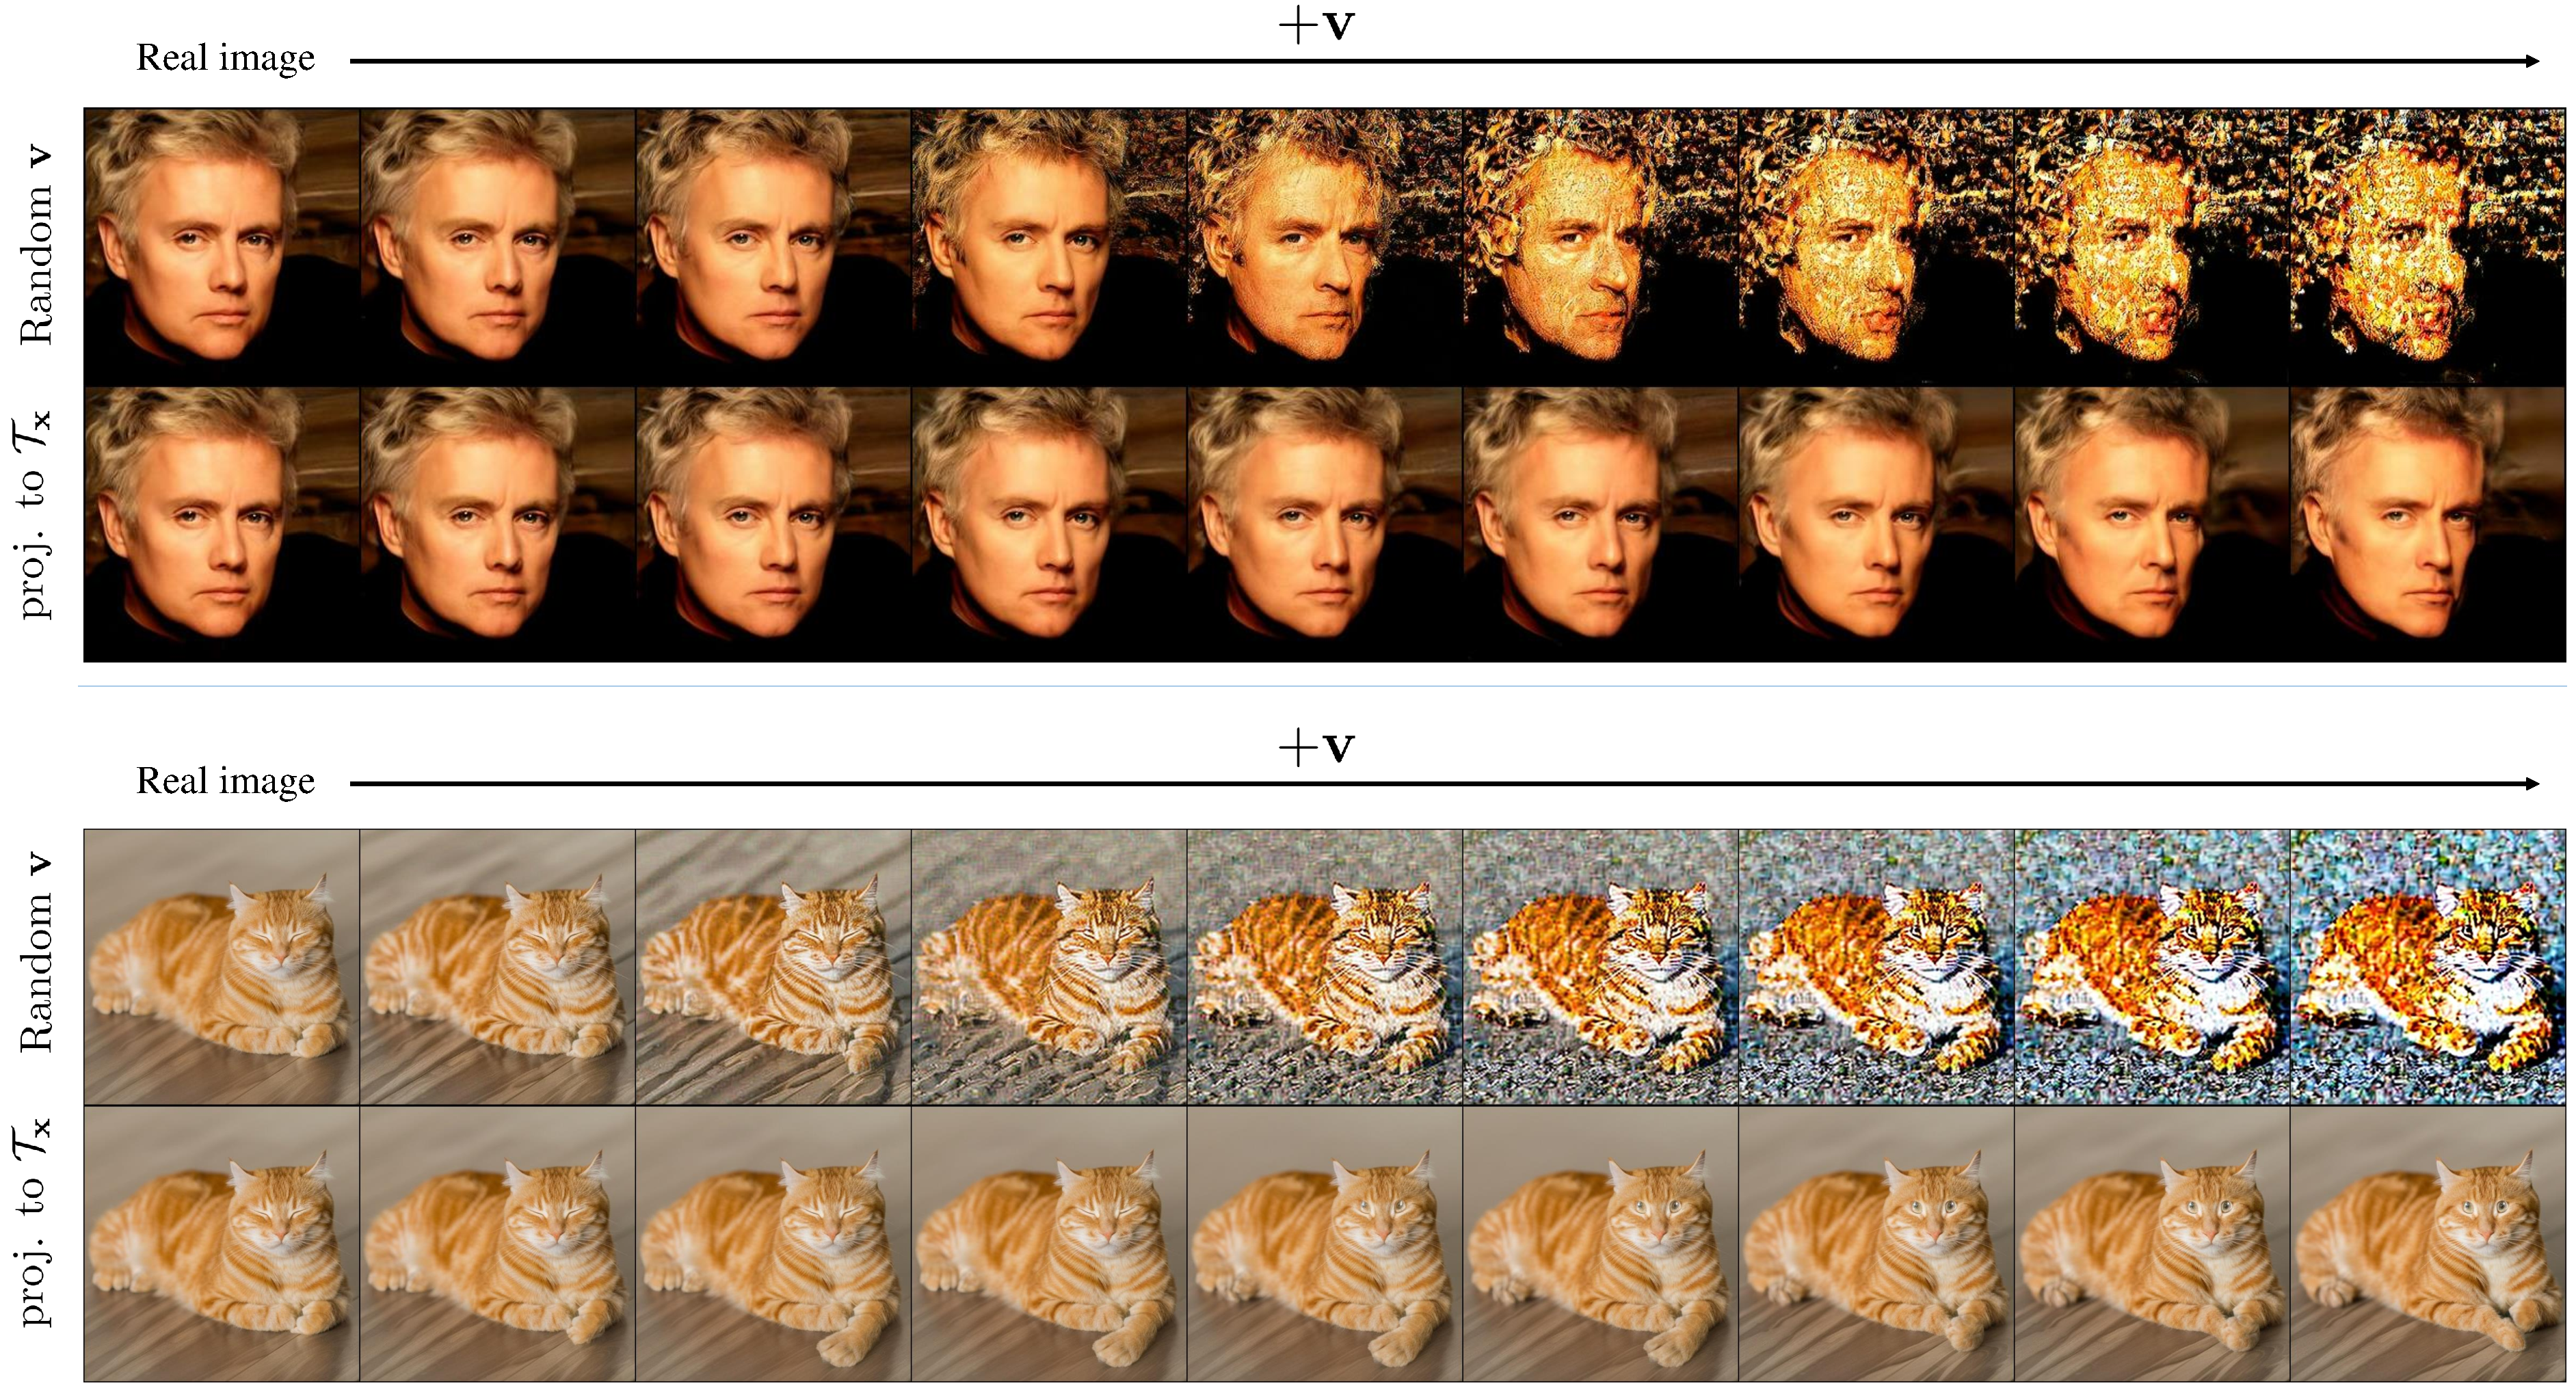
\includegraphics[width=0.9\linewidth]{figure/random_v.pdf}
    \caption{
    \textbf{Importance of the discovered latent directions.} Random direction experiments with CelebA-HQ pre-trained model (top) and Stable Diffusion (bottom).
    % 위 3개 row 는 CelebA-HQ 에서의 결과, 밑은 Stable Diffusion 에서의 결과를 보여주고 있다. 
    %The image on the far left represents the reconstructed original image, while the subsequent images demonstrate the interpretable edits that have been made to it. 
    % {The leftmost image represents the reconstruction of real image. }
    \yh{Adding random directions instead of latent directions severely distorts the resulting images.}
    %As we move towards the right, we impose stronger editing. 
    %When we perform edits along a random direction, the generated image does not change semantically meaningfully.
    {When we perform edits along the projection onto the latent subspace $\mathcal{T}_{\mathbf{x}}$, the generated image presents a semantically meaningful transformation.
    }
    % Projection onto a space orthogonal to the subspace further supports it by showing less semantic change and consistent image distortion.
    }
    \label{fig:random_v}
\end{figure}

\begin{figure}[!t]
    \centering
    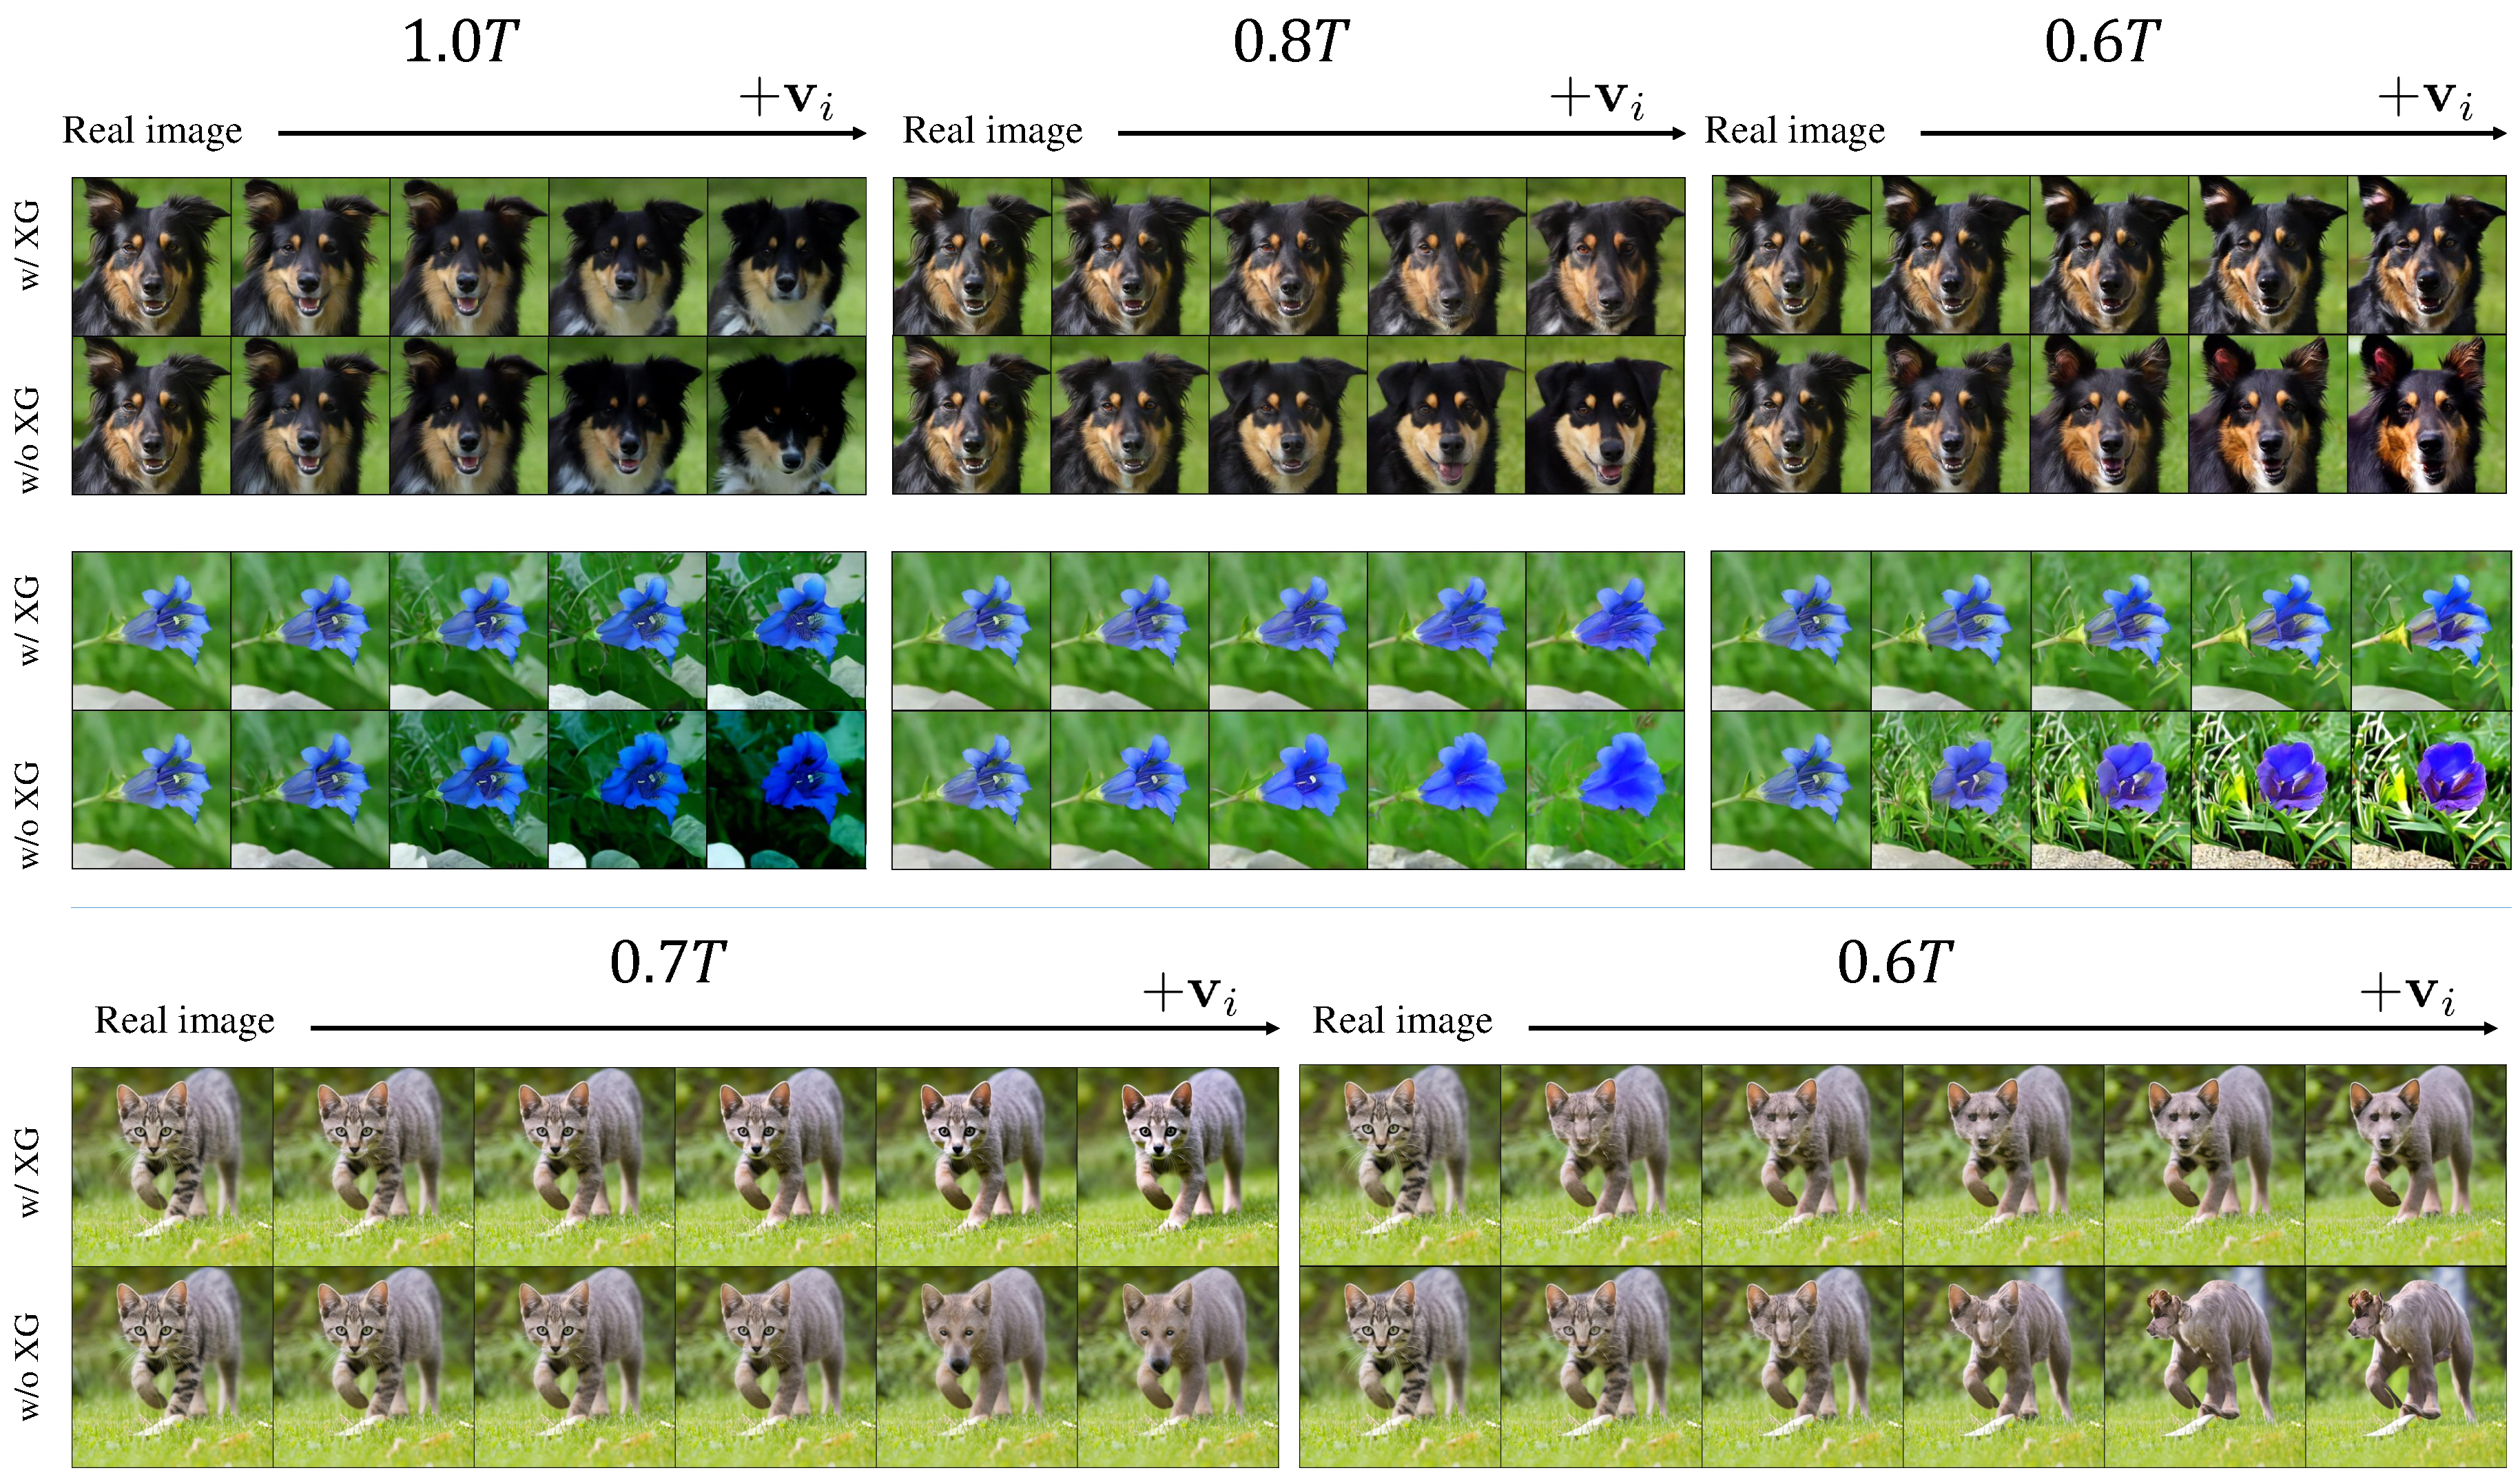
\includegraphics[width=1.0\linewidth]{figure/x_space_guidance.pdf}
    \caption{
    \textbf{Importance of the $\vx$-space guidance.} 
    $\vx$-space guidance experiments with AFHQ (top), Flowers pre-trained model (middle), and Stable Diffusion (bottom).
    $\vx$-space guidance helps achieve qualitatively similar editing while preserving the content of the original image.}
    \label{fig:x_space_guidance}
\end{figure}


\paragraph{$\vx$-space guidance}
\label{appendixsec:ablation_x_guidance}
\fref{fig:x_space_guidance} demonstrates the the effectiveness of $\vx$-space guidance compared to a straightforward alternative: simple addition. First, $\vx$-space guidance produces higher quality images with similar meaning. Especially Stable Diffusion apparently benefits from $\vx$-space guidance regarding smoothness of the editing strength and artifacts. The difference is more significant at $t=0.6T$. Note that the meaning of the same directions may slightly differ between the two settings due to non-linearity of the U-Net.
% To investigate the effectiveness of $\vx$-space guidance, we qualitatively compare it to the na\"ive approach of direct addition. First, as shown in \fref{fig:x_space_guidance}, overall, $\vx$-space guidance allows qualitatively similar manipulations while enhancing their quality. Specifically, we observe that when using $\vx$-space guidance, artifacts are reduced to a greater extent in Stable Diffusion compared to the unconditional model, and the reduction is more significant at $t=0.6T$ compared to $t=T$. However, it is worth noting that the qualitative direction of the manipulations may slightly differ.

Currently, we do not have a deeper understanding of the underlying principles of $\vx$-space guidance. Exploring the reasons behind its ability to improve manipulation quality would be an interesting direction for future work.

% \clearpage


\begin{figure}[!t]
    \centering
    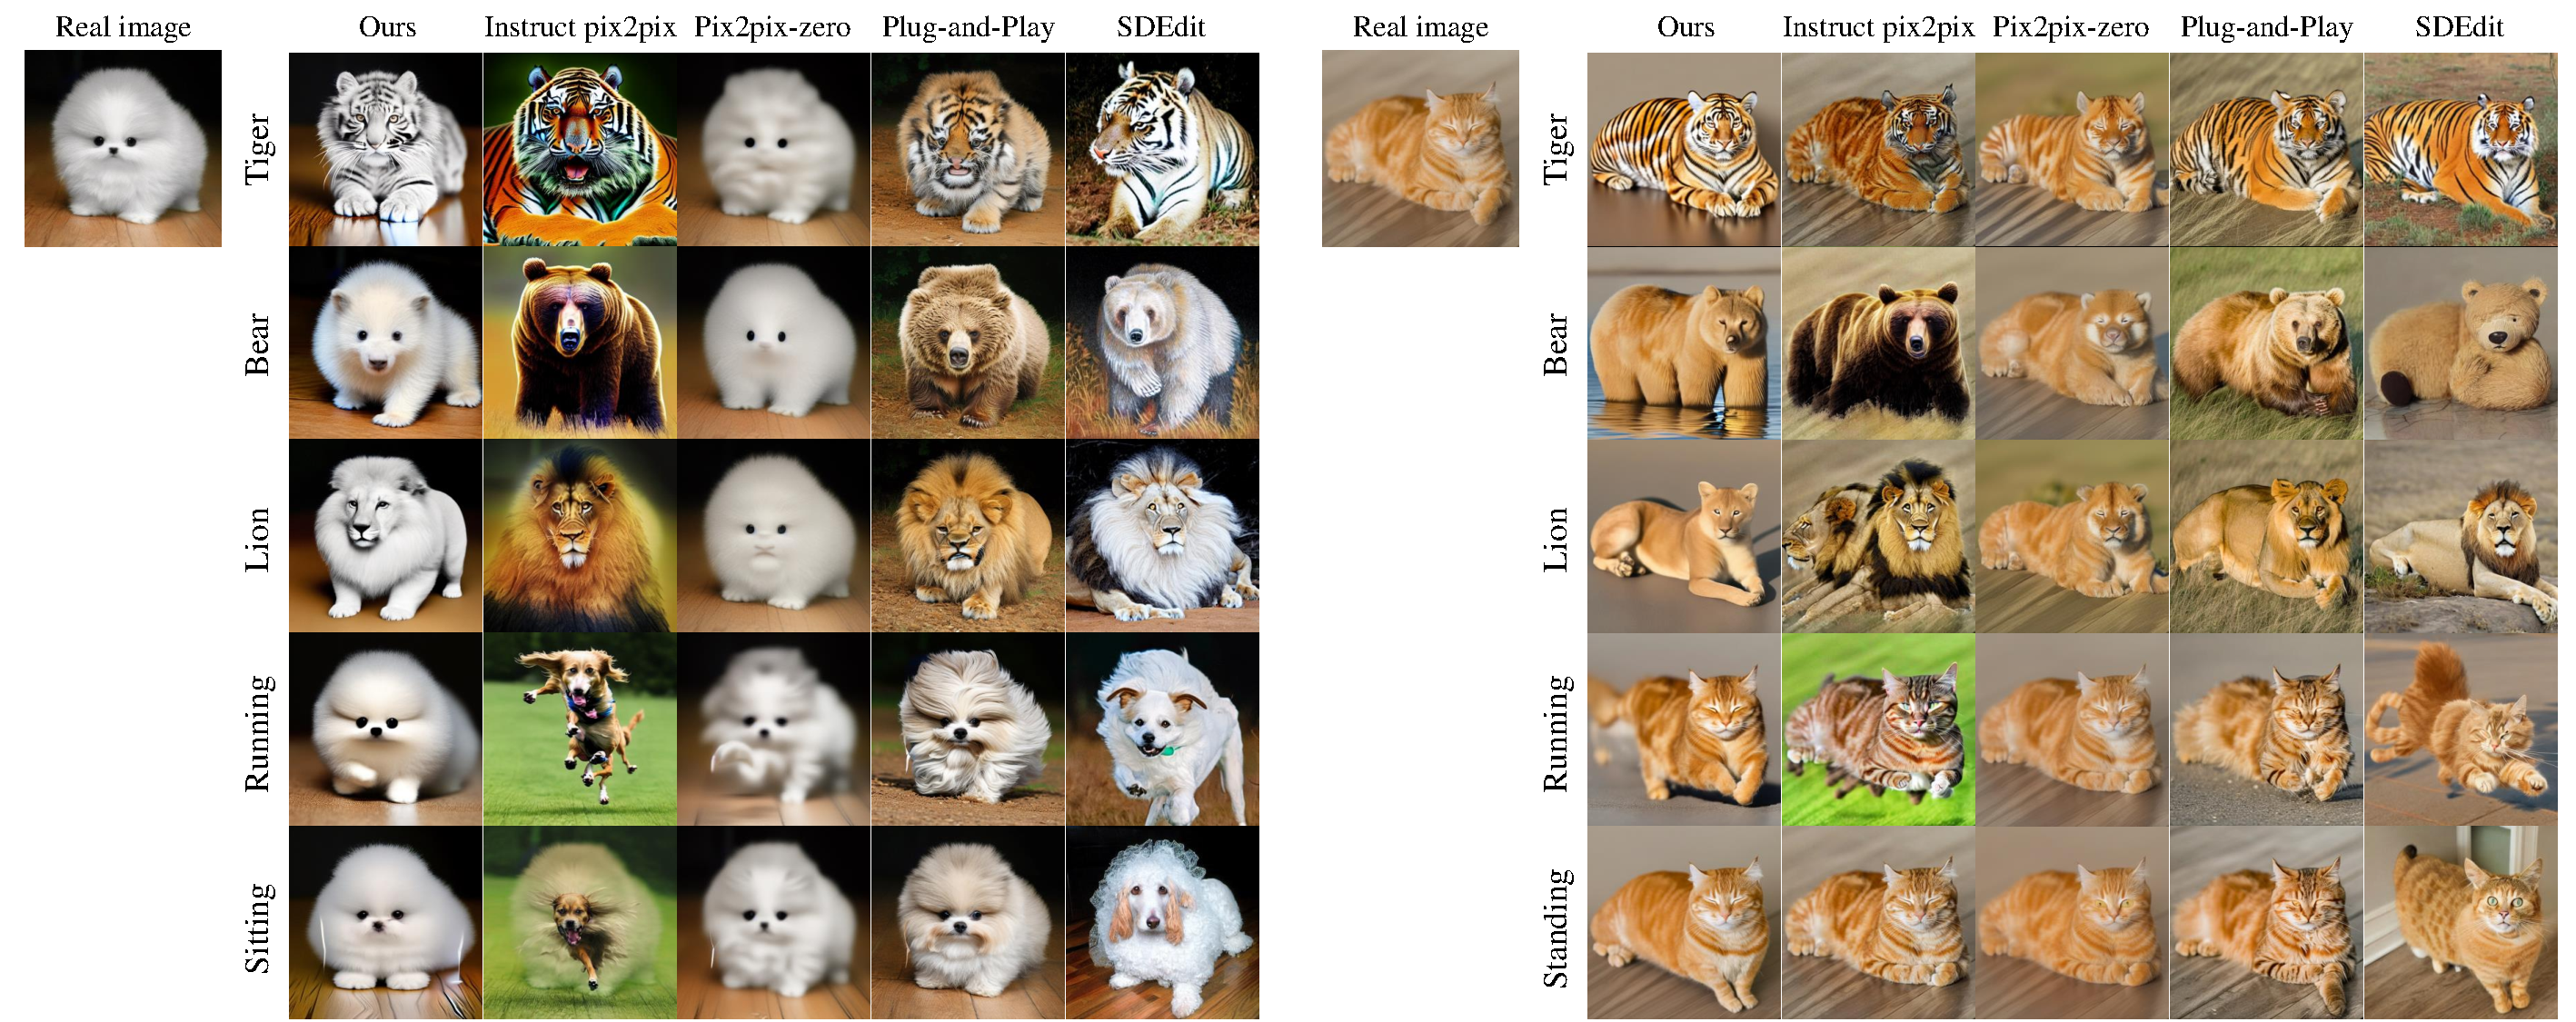
\includegraphics[width=0.95\linewidth]{figure/comparison_rebuttal.pdf}
    \caption{
    \textbf{Comparison with various image editing methods.}
    Our approach empowers image editing that aligns seamlessly with text conditions while upholding object identity. In contrast, alternative methods exhibit deficiencies such as: inadequate preservation of object structure (Instruct pix2pix), inefficacious manipulation (Pix2pix-zero), or challenges in maintaining identity fidelity (Plug-and-Play, SDEdit).
    }
    %\caption{\textbf{Comparison with different image editing methods.} Our method enables image editing that aligned with text conditions while preserving object identity. In contrast, other methods have shortcomings like: not preserving object structure (Instruct pix2pix), failing to manipulate effectively (Pix2Pix-zero), or having issues with less preserved identity (Plug-and-Play).}
    % \vspace{0.2em}
    \label{fig:comparison}
\end{figure}

\section{Comparative experiment to other state-of-the-art (SoTA) editing methods}
\label{appendix:comparisons}
We conduct qualitative comparisons with text-guided image editing methods. Our SoTA baseline methods include: (i) SDEdit \cite{meng2021sdedit}, (ii) Pix2Pix-zero \cite{parmar2023zero}, (iii) PnP \cite{tumanyan2022plug}, and (iv) Instruct Pix2Pix \cite{brooks2023instructpix2pix}. All comparisons were performed using the official code.
Please refer to \fref{fig:comparison} for the qualitative results.

We also compare the time complexity of each method. For a fair comparison, we only identify the first singular vector $\mathbf{v}_1$, i.e., $n=1$, and set the number of DDIM steps to 50. All experiments were conducted on an Nvidia RTX 3090. The runtime for each method is summarized in \tref{tab:comparison_time}.

The computation cost of our method remains comparable to other approaches, although the Jacobian approximation takes around 2.5 seconds for $n=1$. This is because we only need to identify the latent basis vector once at a specific timestep. Furthermore, our approach does not require additional preprocessing steps like generating 100 prompts with GPT and obtaining embedding vectors (as in Pix2Pix-zero), or storing feature vectors, queries, and key values (as in PnP). Our method also does not require finetuning (as in Instruct Pix2Pix). This leads to a significantly reduced total editing process time in comparison to other methods.

\begin{table}[t]
\caption{\modify{\textbf{Comparisons of the time complexity of state-of-the-art editing methods} 
% We used five attribution methods, including a random baseline, to compare the rankings. 
% A stronger correlation between the rankings signifies greater consistency in the results, irrespective of whether the model undergoes retraining or not.
}}
% \vskip 0.15in
\begin{center}
\begin{small}
\begin{tabular}{c|c|c}
\toprule
 Image Edit Method & Running time & Preprocessing \\
\midrule
Ours             &     11 sec    & N/A            \\
SDEdit           &      4 sec    & N/A            \\
Pix2Pix-zero     &     25 sec    & 4 min          \\
PnP              &     10 sec    & 40 sec         \\
Instruct Pix2Pix &     11 sec    & N/A            \\
\bottomrule
\end{tabular}
\end{small}
\end{center}
% \vskip -0.1in
\label{tab:comparison_time}
\end{table}


\section{More Discussions}

% \begin{wrapfigure}{!r}{6cm}
%     \vspace{-1.5em}
%     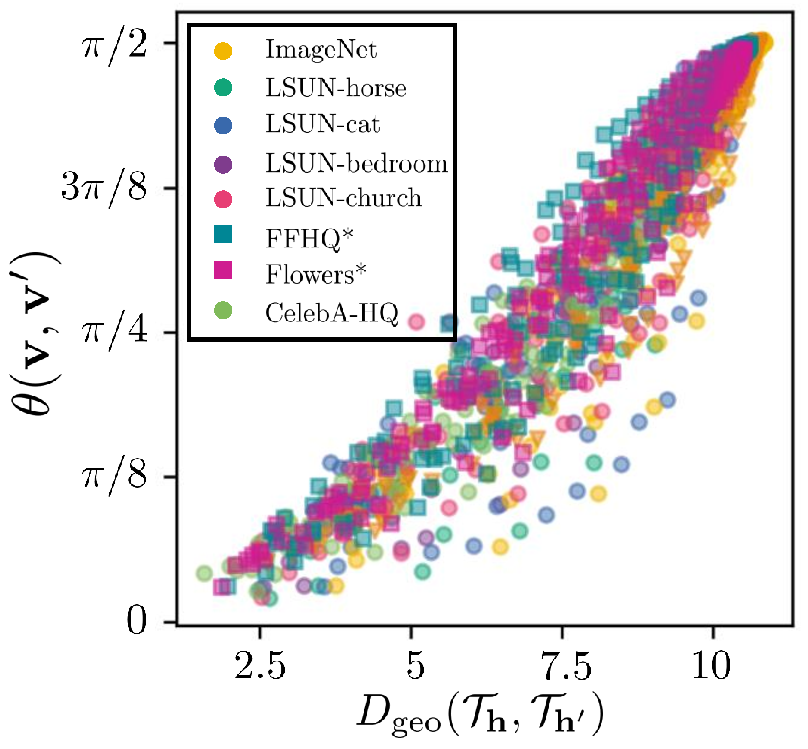
\includegraphics[width=6cm]{figure/parallel_transport_x_theta.pdf}
%     \vspace{-1.5em}
%     \caption{\textbf{Parallel transport between similar tangent spaces creates similar latent directions.}
%     The horizontal axis represents the geodesic distance between tangent spaces from different timesteps, while the vertical axis represents the angle between the original latent direction and transported latent direction. 
%     Different colors represent various datasets. 
%     A positive relationship is observed between tangent space distance and the distortion induced by parallel transport.}
%     \label{fig:parallel_transport_x_theta}
%     \vspace{-2.5em}
% \end{wrapfigure} 

\begin{figure}[!t]
\centering
    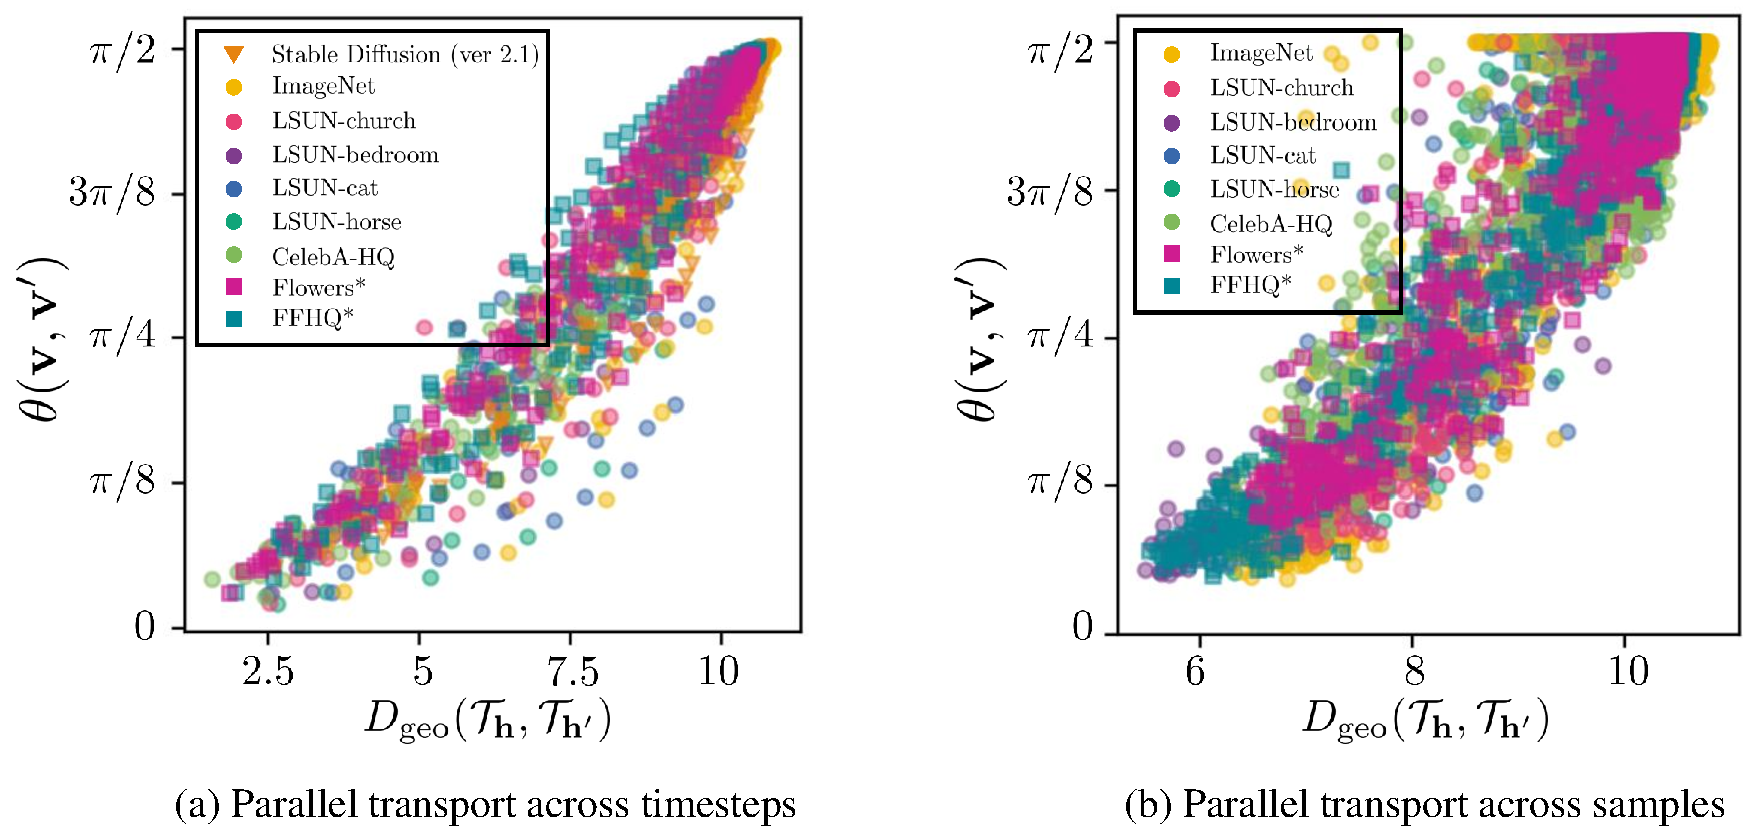
\includegraphics[width=0.95\linewidth]{figure/parallel_transport_x_theta_long.pdf}
    \vspace{-0.5em}
    \caption{
    \textbf{Parallel transport between similar tangent spaces creates similar latent directions.} 
    The horizontal axis represents the geodesic distance between tangent spaces from (a) different timesteps (b) different samples at $t \in \{T, 0.9T, \cdots, 0.1T\}$. The vertical axis represents the angle between the original latent direction and transported latent direction. 
    Different colors represent various datasets. 
    A positive relationship is observed between tangent space distance and the distortion induced by parallel transport.
    }
    \label{fig:parallel_transport_x_theta}
    % \vspace{-1em}
\end{figure}

\paragraph{Why do we measure the geodesic distance of the tangent spaces instead of the latent subspaces?}
\label{appendixsec:relationship_tangent_latent}
The geodesic distance on the Grassmannian manifold between two subspaces is defined as the $l_{2}$-norm of principal angles. 
To define angles between different vector spaces, an inner product needs to be defined. In our work, we define the inner product in $\mathcal{T}_\vx$ using the pullback metric. The issue is that the pullback metric is locally defined for each latent subspace $\mathcal{T}_\vx$ (\eref{eq:pullback}). Therefore, measuring angles between distant latent subspaces becomes challenging. On the other hand, \ehspace{} follows the assumption of the Euclidean metric. Consequently, even for distant tangent spaces, angles can be easily computed using the dot product.
In this regard, we measure the similarity between latent subspaces by exploiting the geodesic distance of their corresponding tangent spaces.
\yh{Furthermore, when compared to \exspace{}, \ehspace{} offers the advantage of being a semantic space, making it more suitable for measuring semantic similarity.}

% In our work, much of the analysis consists of measuring the geodesic distance between different tangent spaces, i.e., $D_{\text{geo}}(\mathcal{T}_\vh, \mathcal{T}_{\vh'})$. 
% This is because the geodesic distance measure the principle angle, based on the dot product. (See \aref{appendixsec:algorithm}). This makes sense in \ehspace{}, where the Euclidean metric is assumed, but not in \exspace{}.


\begin{figure}[!t]
\centering
    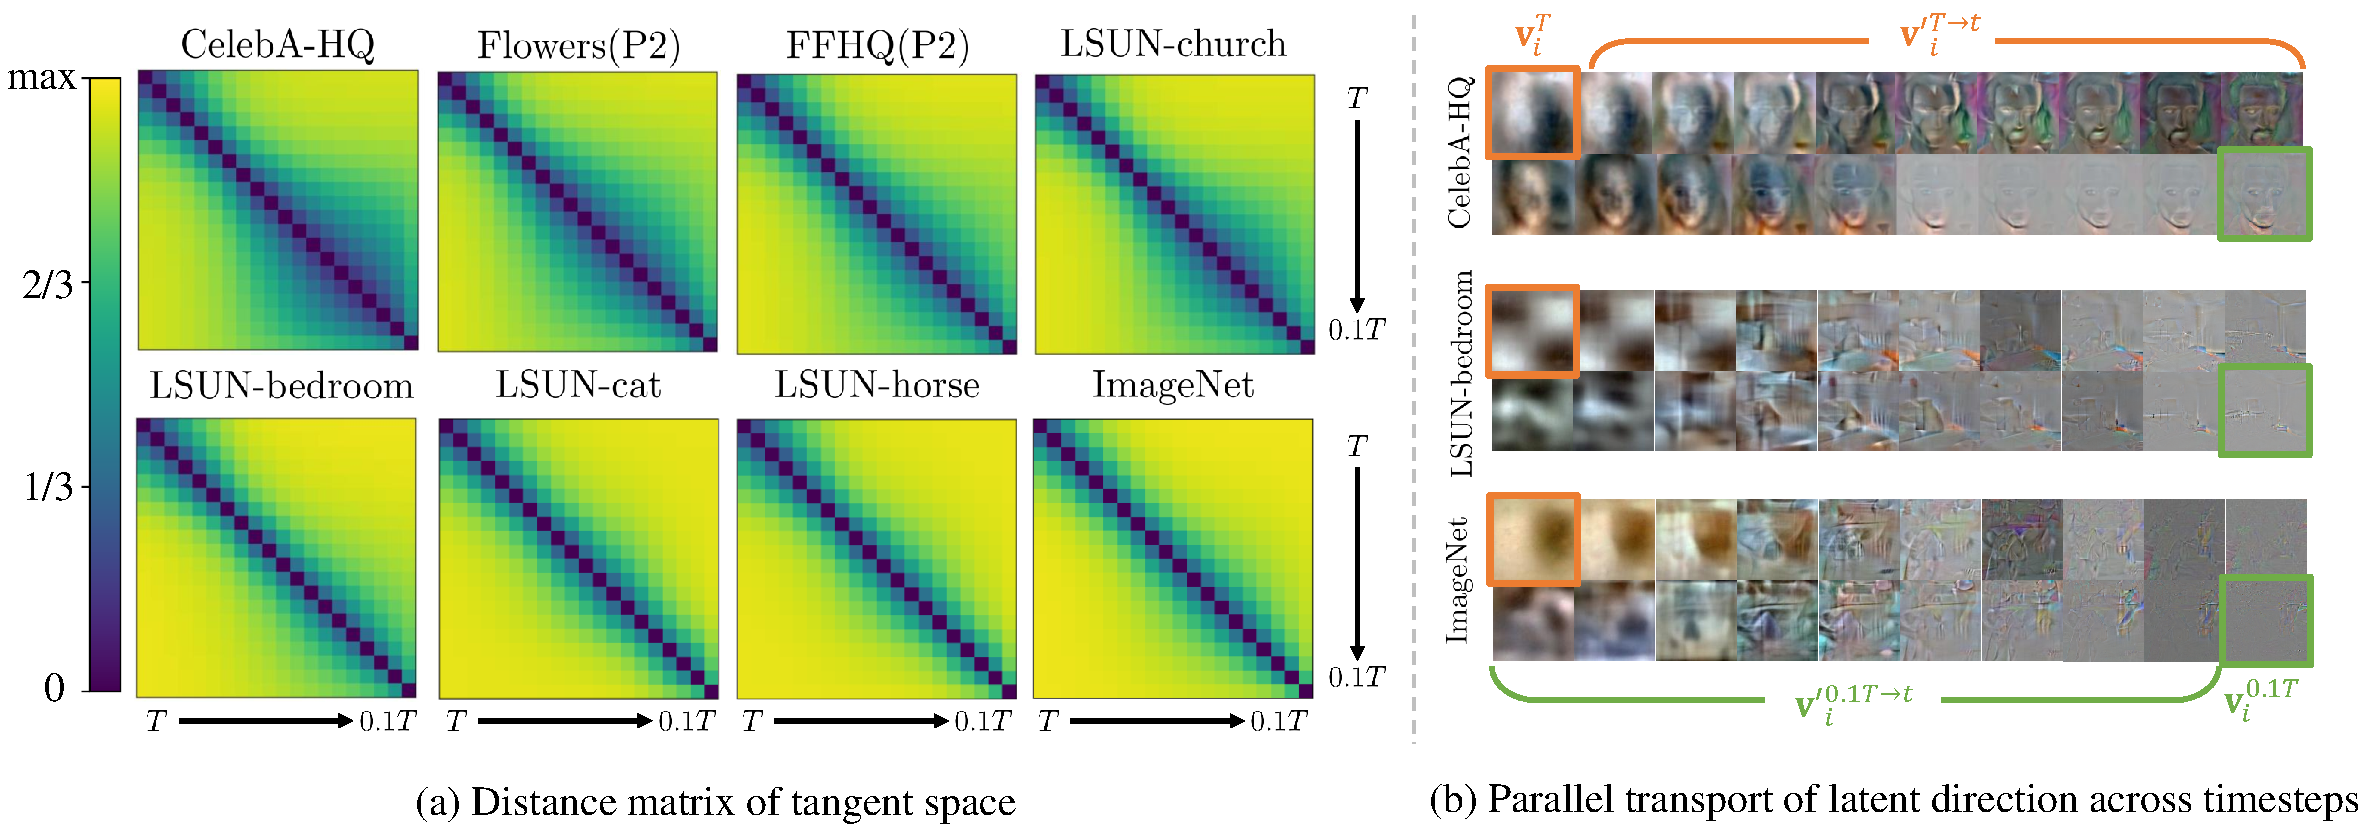
\includegraphics[width=0.95\linewidth]{figure/evolution-t-appendix.pdf}
    \vspace{-0.5em}
    \caption{
    \textbf{More examples of tangent spaces across diffusion timesteps.} 
    (a) Distance matrix visualization of tangent space measured by geodesic metric across various timesteps.
    (b) Visualization of the result from parallel transport across timesteps.
    \yh{${\vv'}_i^{t_a \rightarrow t_b}$ denotes the latent vector transported from $t_a$ to $t_b$.
    Transported vector significantly deviates from the original vector, as the tangent space grows further apart according to the distance matrix. 
    For visualization purposes, $\vv_i$ \jo{is min-max normalized}.}}
    \label{fig:evolution-t-appendix}
    % \vspace{-1em}
\end{figure}


\paragraph{Similar tangent space implies similar latent subspace}
% \paragraph{What does it imply if the tangent space is similar?}
% In \fref{fig:parallel_transport_x_theta}, 서로 다른 timestep 에서 구한 tangent space 간 geodesic distance 와 그 둘 사이에서 parallel transport 한 latent direction 간 각도를 구한 것이다. 
% It is evident that as the geodesic distance decreases, the amount of distortion during parallel transport also reduces.
% \yh{이는 tangent space 가 유사하면 latent subspace 도 유사함을 의미한다.}
In \fref{fig:parallel_transport_x_theta}, we calculated the geodesic distance of tangent spaces obtained at different timesteps (or different samples at same the timestep) and the angle between the original latent direction and parallel transported direction between them.
It is evident that as the geodesic distance decreases, the amount of distortion during parallel transport also reduces.
% For parallel transport across different timesteps, the result is visually illustrated in \fref{fig:evolution-t-appendix}.

\modify{
Notice that the similarity between tangent spaces implies \uh{consistency of latent basis across timesteps}. %a consistent latent basis at each timestep.
In \fref{fig:evolution-t-appendix} (b), we parallel transport the latent vector $\vv_i$ to various tangent spaces and visualize the outcomes.
As expected, when the tangent spaces are similar, the transported vector ${\vv'}_i$ retains the original signal. On the other hand, as we move to more distant timesteps, where the tangent space is farther apart, ${\vv'}_i$ deviates from the original signal.
}



% Furthermore, \fref{fig:Homogenity_prompts_appendix}, we visualize latent direction given various prompts.
% 여기서도 마찬가지로, tangent space 간 거리가 가까워지는 0.6T 구간부터 latent direction 들이 유사해지는 양상을 확인할 수 있었다. 

% \label{appendixsec:relationship_tangent_latent}
% 두 tangent space 가 유사하다는건 그에 대응하는 latent space 에서 유사한 signal 을 찾을 수 있음을 의미합니다. 
% In \fref{fig:Homogenity_prompts_appendix}, 는 서로 다른 timestep 에서 tangent space $\mathcal{T}_\vh, \mathcal{T}_{\vh'}$ 를 뽑고, 하나의 tangnet space 에서 다른 tangent space 로 parallel transport 한 뒤, .
% Parallel transport 를 할 때 geodesic distance 가 작을수록 왜곡이 덜 일어나는 것은 자명하다. 하지만, \fref{fig:Homogenity_prompts_appendix} 는 latent vector 도 왜곡이 덜 일어남을 말해주고 있다. \fref{fig:evolution-t-appendix} 는 이 결과를 눈으로 보여주고 있다. 

% 또한 \fref{fig:Homogenity_prompts_appendix} 는 서로 다른 prompt 가 주어졌을때 latent vector 를 눈으로 보여주고 있다. tangent space 간 distance 가 클수록, latent vector 에 담긴 패턴이 많이 달라지는 것을 확인할 수 있다.

% \begin{figure}[!b]
% \centering
%     \vspace{-1.5em}
%     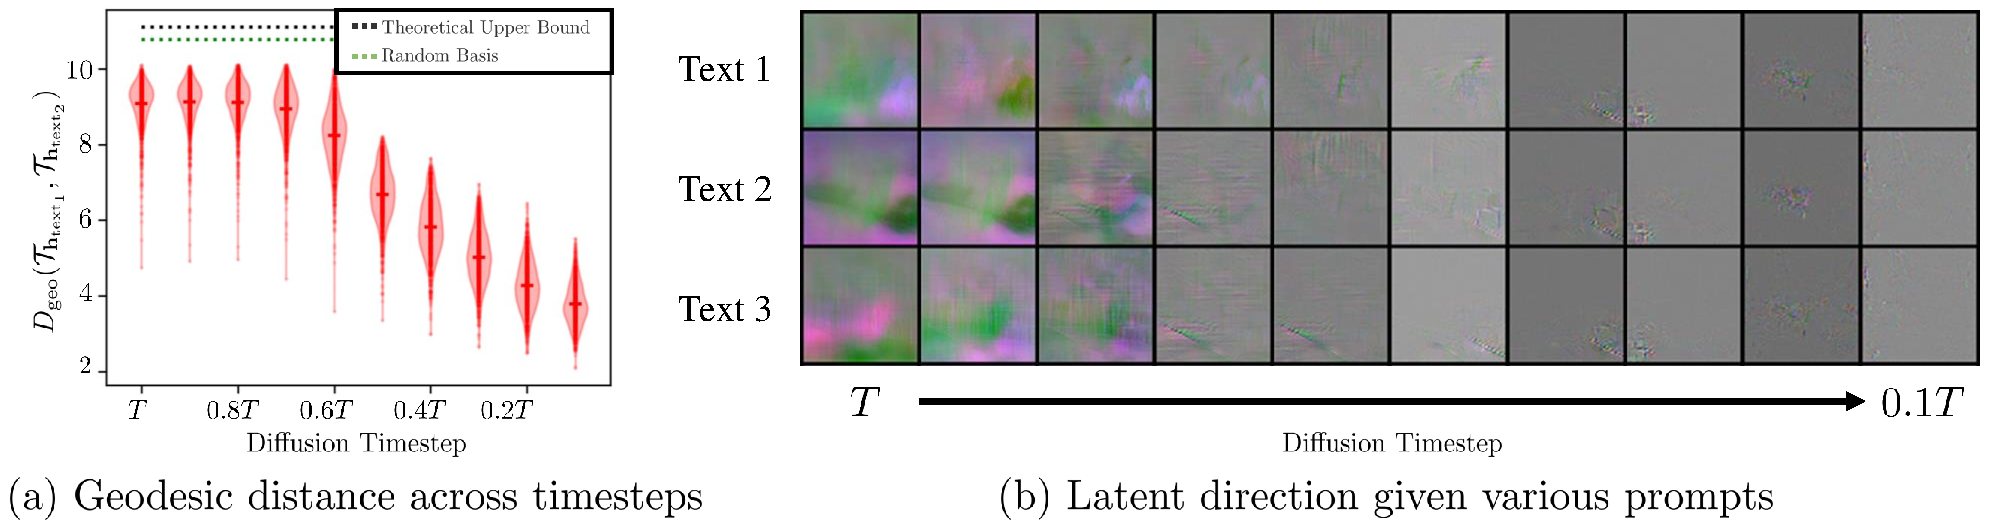
\includegraphics[width=0.95\linewidth]{figure/Homogenity_prompts_appendix.pdf}
%     \vspace{-0.5em}
%     \caption{
%     \textbf{More examples of image editing using the latent basis.} 
%     (a) Each point represents the distance between tangent spaces created from
%     different prompts. Until around t = 0.7T, the distance between tangent spaces is very large, but it gradually decreases thereafter.
%     (b) Visualization of the top latent direction from various text conditions. It shows that as the timestep exceeds 0.6T, the latent direction gradually becomes more similar.
%     }
%     \label{fig:Homogenity_prompts_appendix}
%     \vspace{-1.5em}
% \end{figure}

% \clearpage

\section{Algorithms}
\label{appendixsec:algorithm}

In this section, for reproducibility purposes, we provide the code for two important algorithms. The code is implemented using PyTorch \cite{paszke2017automatic}.

\paragraph{Jacobian subspace iteration}
The diffusion model has dimensions that are too large in both \exspace{} and \ehspace{}, making the computation of the Jacobian infeasible. To overcome this challenge, we attempt the Jacobian subspace iteration algorithm to approximate the singular value of the Jacobian, as proposed in \cite{haas2023discovering}. For details, please refer to \citet{haas2023discovering}.

\begin{lstlisting}[language=Python, caption=Python example, caption={\textbf{Jacobian subspace iteration}}, captionpos=b]
import torch # >= ver 2.0

def local_encoder_pullback(
        x, t, get_h, n=50, chunk_size=25, min_iter=10, max_iter=100, convergence_threshold=1e-4,
    ):
    '''
    Args
        - x : tensor ; latent variable
        - t : tensor ; diffusion timestep
        - get_h : function ; return h given x, t
        - n ; low-rank approximation dimension
        - chunk_size ; To avoid OOM error
        - min_iter (max_iter) ; minimum (maximum) number of iteration
        - convergence_threshold ; to check convergence of power-method
    '''
    # set number of chunk to avoid OOM
    num_chunk = n // chunk_size + 1

    # get dimensions of x space and h space
    h_shape = get_h(x, t).shape
    c_i, w_i, h_i = x.size(1), x.size(2), x.size(3)
    c_o, w_o, h_o = h_shape[1], h_shape[2], h_shape[3]

    # power-method
    a = torch.tensor(0., device=x.device, dtype=x.dtype)
    vT = torch.randn(c_i*w_i*h_i, n, device=x.device)
    vT, _ = torch.linalg.qr(vT)
    v = vT.T
    v = v.view(-1, c_i, w_i, h_i)

    for i in range(max_iter):
        v = v.to(device=x.device, dtype=x.dtype)
        v_prev = v.detach().cpu().clone()
        
        time_s = time.time()
        u = []
        v_buffer = list(v.chunk(num_chunk))
        for vi in v_buffer:
            g = lambda a : get_h(x + a*vi, t=t)
            ui = torch.func.jacfwd(
                g, argnums=0, has_aux=False, randomness='error'
            )(a)
            u.append(ui.detach().cpu().clone())
        u = torch.cat(u, dim=0)
        u = u.to(x.device, x.dtype)

        g = lambda x : torch.einsum(
            'b c w h, i c w h -> b', u, get_h(x, t=t)
        )
        v_ = torch.autograd.functional.jacobian(g, x)
        v_ = v_.view(-1, c_i*w_i*h_i)

        _, s, v = torch.linalg.svd(v_, full_matrices=False)
        v = v.view(-1, c_i, w_i, h_i)
        u = u.view(-1, c_o, w_o, h_o)
        
        convergence = torch.dist(v_prev, v.detach().cpu()).item()
        if torch.allclose(v_prev, v.detach().cpu(), atol=convergence_threshold) and (i > min_iter):
            break

    # reshape as a x space, h space vector
    u, s, vT = u.reshape(-1, c_o*w_o*h_o).T.detach(), s.sqrt().detach(), v.reshape(-1, c_i*w_i*h_i).detach()
    return u, s, vT
\end{lstlisting}

\paragraph{Geodesic metric}
For a detailed discussion on the geodesic metric, please refer to \citet{choi2021not} for more information.
% Geodesic metric 에 대한 구체적인 논의는 \citet{} 를 참고하라. 

\begin{lstlisting}[language=Python, caption={\textbf{Geodesic metric}}]
import torch

def geodesic_metric(U1, U2):
    _, S, _ = torch.linalg.svd(U1.T @ U2)
    th = torch.acos(S)
    return th.norm()
\end{lstlisting}

% power-method approximation
% \begin{algorithm}[ht!]
% \caption{Feature Direction}
% \label{alg:local_basis}
% \begin{algorithmic}[1]
% \REQUIRE {latent variable $\mathbf{x}$, timestep $t$, U-Net encoder $f : \mathcal{X} \times T \rightarrow \mathcal{H}$, Feature direction index $i$}
% \STATE {$J$             = Jacobian($f(\cdot, t)$)($\mathbf{x}$)}
% \STATE $U, S, V^{\tran}$ = SingularValueDecomposition($J$) 
% \STATE {$\mathbf{v}_i, \mathbf{u}_i$ = $V^{\tran}$[$i$, :], $U$[:, $i$]}
% \STATE {{\bfseries Return} $\mathbf{v}_i, \mathbf{u}_i$}
% \end{algorithmic}
% \end{algorithm}

%%%%%%%%%%%%%%%%%%%%%%%%%%%%%%%%%%%
% below is the additional figures %
%%%%%%%%%%%%%%%%%%%%%%%%%%%%%%%%%%%
\clearpage

\section{Additional results}
\label{appendix:additional_results}
\subsection{Latent basis}
\label{appendix:local}
\paragraph{Unconditional latent basis}
We provide more examples of image editing using the latent basis. Figure~\ref{fig:ffhq_vis}, \ref{fig:afhq_vis}, \ref{fig:flowers_vis}, \ref{fig:stable_7T} and \ref{fig:stable_6T} show that every latent basis produces different results and editing at timestep $T$ yields coarse changes while 0.6$T$ leads to fine changes. Stable Diffusion shows a similar trend; 0.7$T$ yields coarse changes while 0.6$T$ leads to fine changes. The results of $T$ in Stable Diffusion will be covered in the \sref{appen:more_discussion}. Please zoom in for the best view.

\begin{figure}[!h]
    \centering
    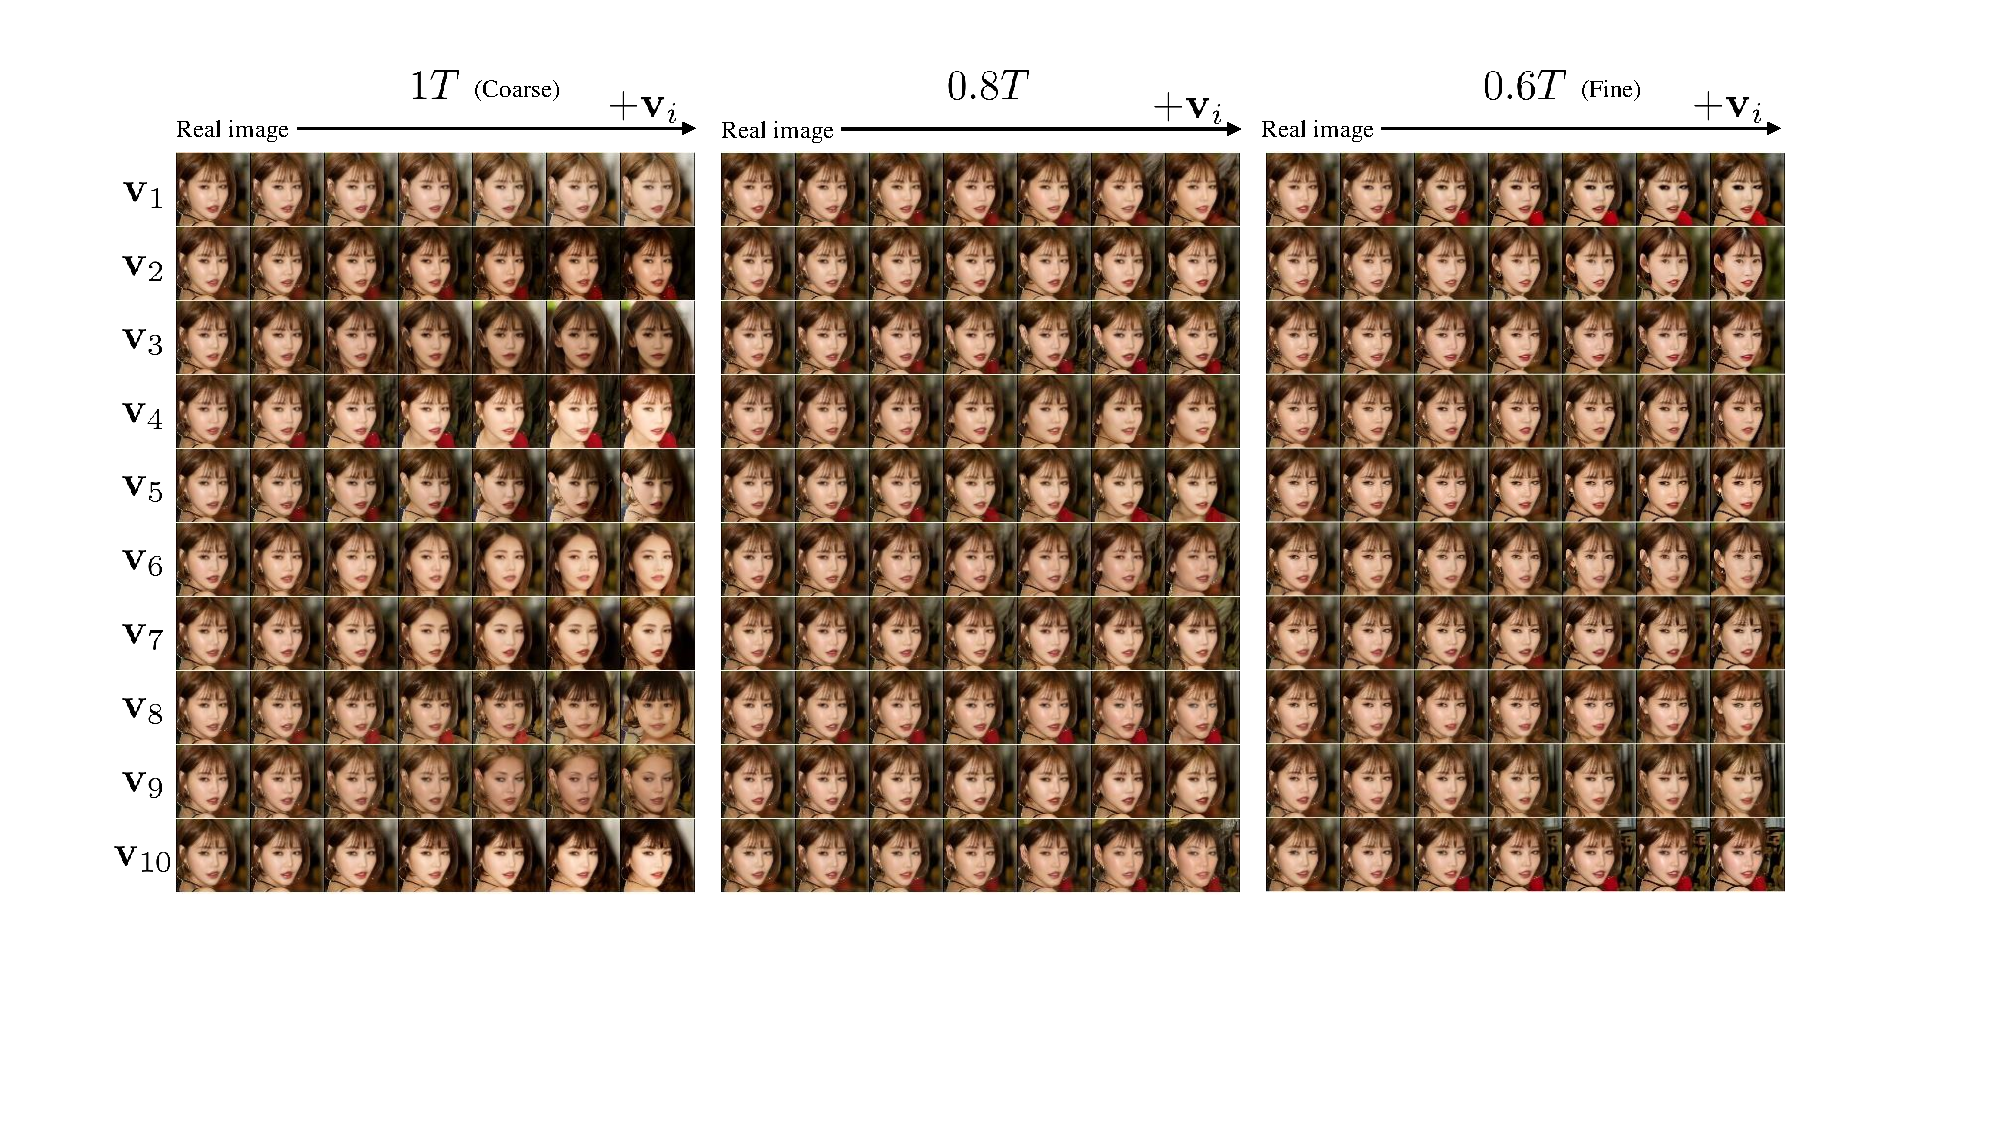
\includegraphics[width=1.0\linewidth]{figure/ffhq_vis.pdf}
    \vspace{-2em}
    \caption{
    \textbf{More examples of image editing using the latent basis in FFHQ.} The editing result using ten $\vv_i$' in FFHQ.  Each column represents edits made at different diffusion timesteps (0.6$T$, 0.8$T$, and 1$T$). Editing at timestep 1$T$ yields coarse changes. On the other hand, editing at timestep 0.6$T$ leads to fine changes. Please zoom in for the best view.}
    \label{fig:ffhq_vis}
\end{figure}

\begin{figure}[!h]
    \centering
    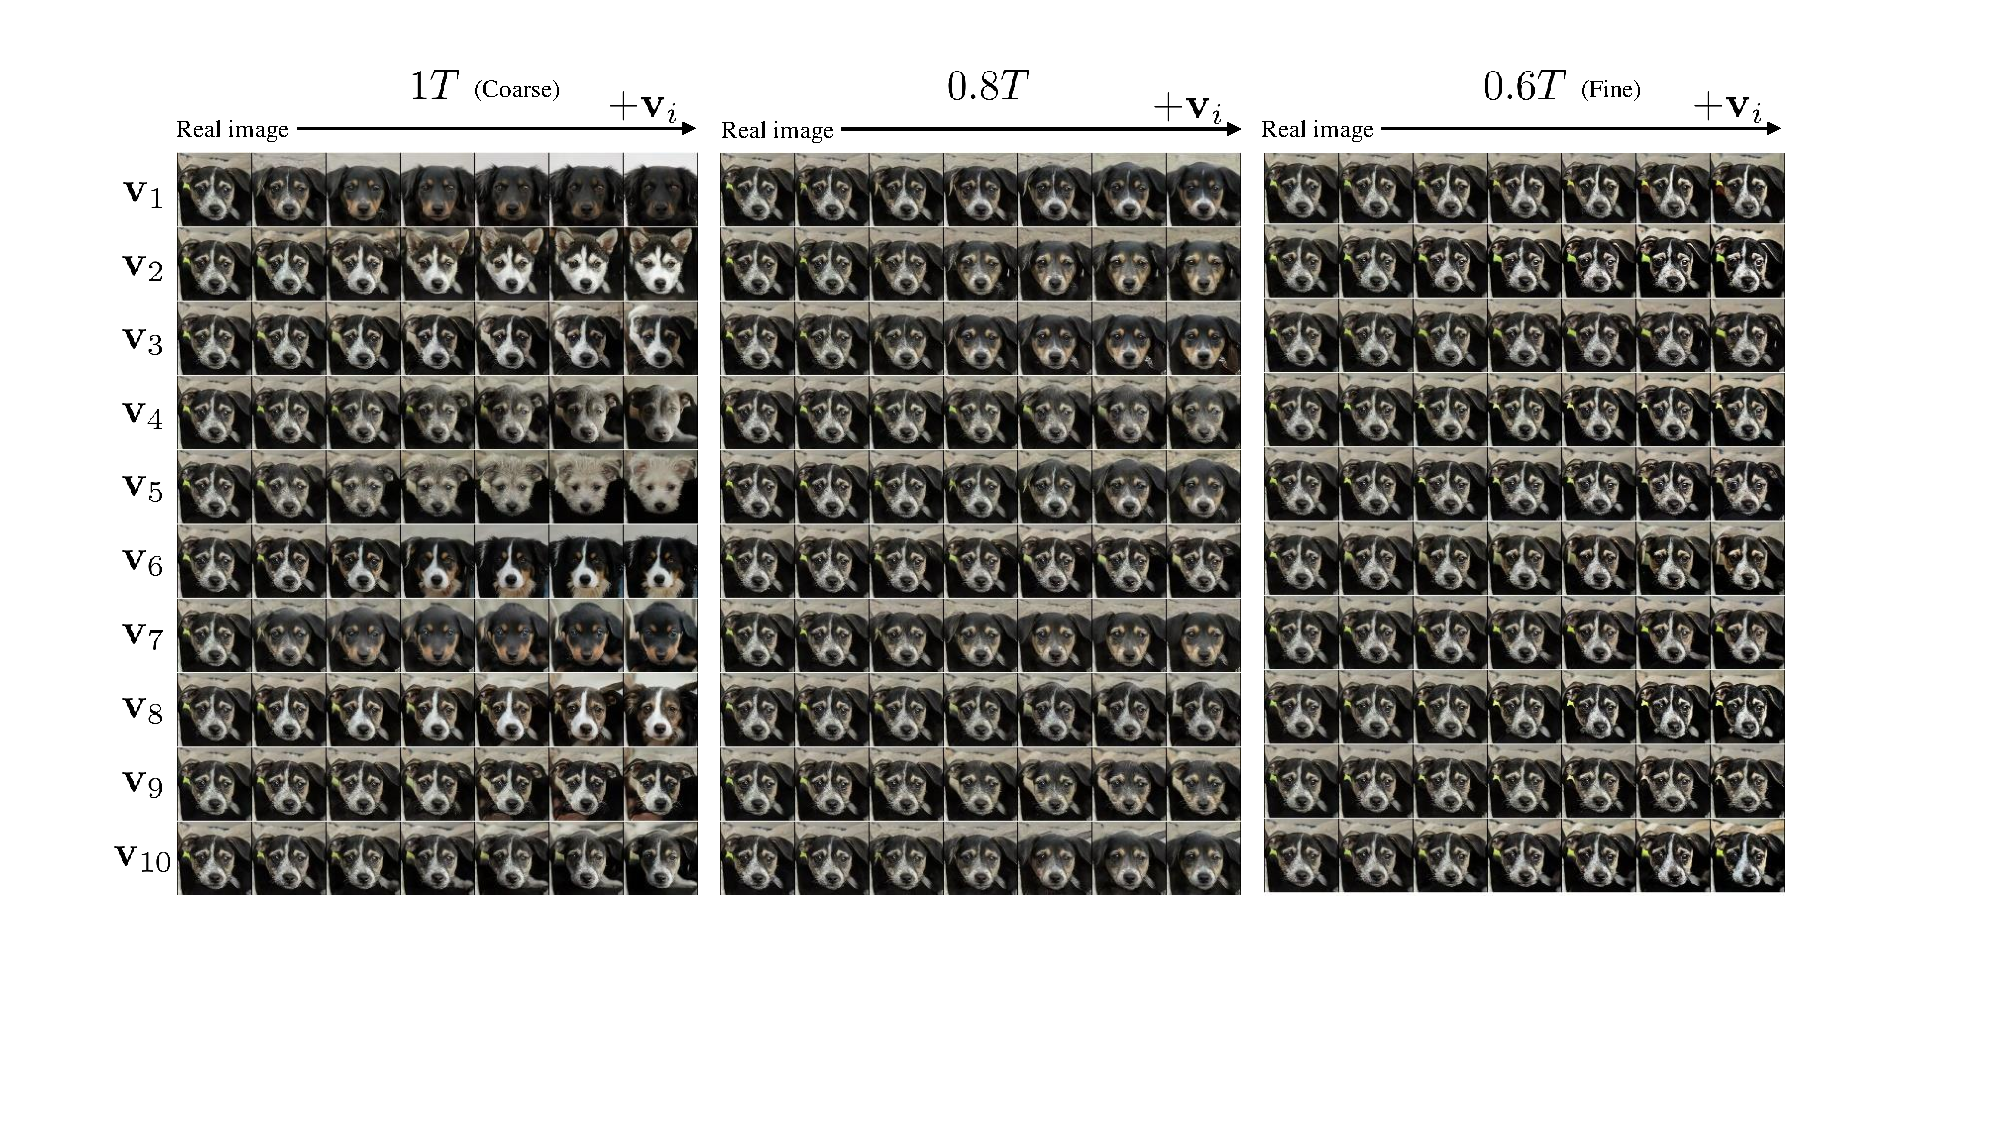
\includegraphics[width=1.0\linewidth]{figure/afhq_vis.pdf}
    \caption{
    \textbf{More examples of image editing using the latent basis in AFHQ.} The editing result using ten $\vv_i$' in AFHQ.  Each column represents edits made at different diffusion timesteps (0.6$T$, 0.8$T$, and 1$T$). Editing at timestep 1$T$ yields coarse changes. On the other hand, editing at timestep 0.6$T$ leads to fine changes. Please zoom in for the best view.}
    \label{fig:afhq_vis}
\end{figure}

\begin{figure}[!h]
    \centering
    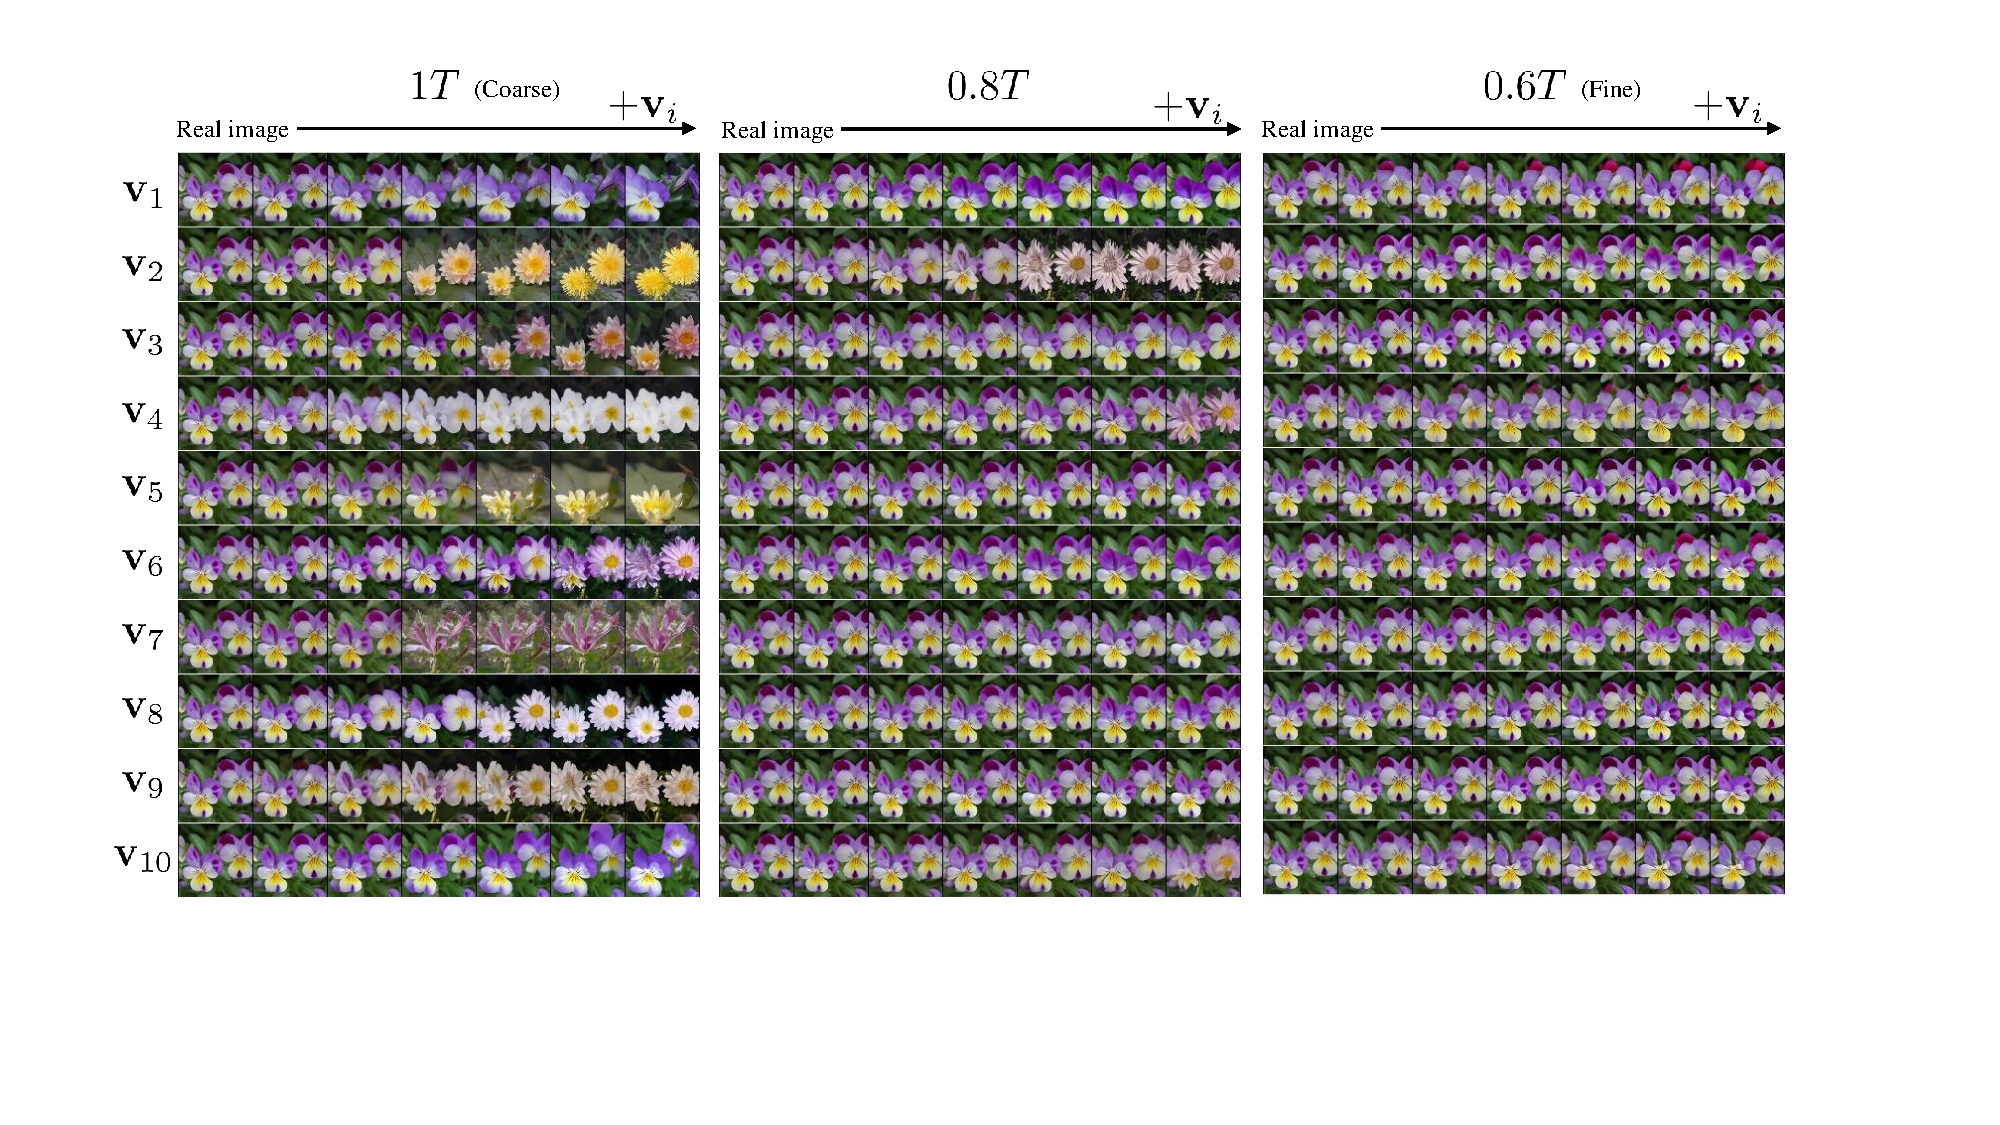
\includegraphics[width=1.0\linewidth]{figure/flowers_vis.pdf}
    \caption{
    \textbf{More examples of image editing using the latent basis in Flowers.} The editing result using ten $\vv_i$' in Flowers.  Each column represents edits made at different diffusion timesteps (0.6$T$, 0.8$T$, and 1$T$). Editing at timestep 1$T$ yields coarse changes. On the other hand, editing at timestep 0.6$T$ leads to fine changes. Please zoom in for the best view.}
    \label{fig:flowers_vis}
\end{figure}

\begin{figure}[!h]
    \centering
    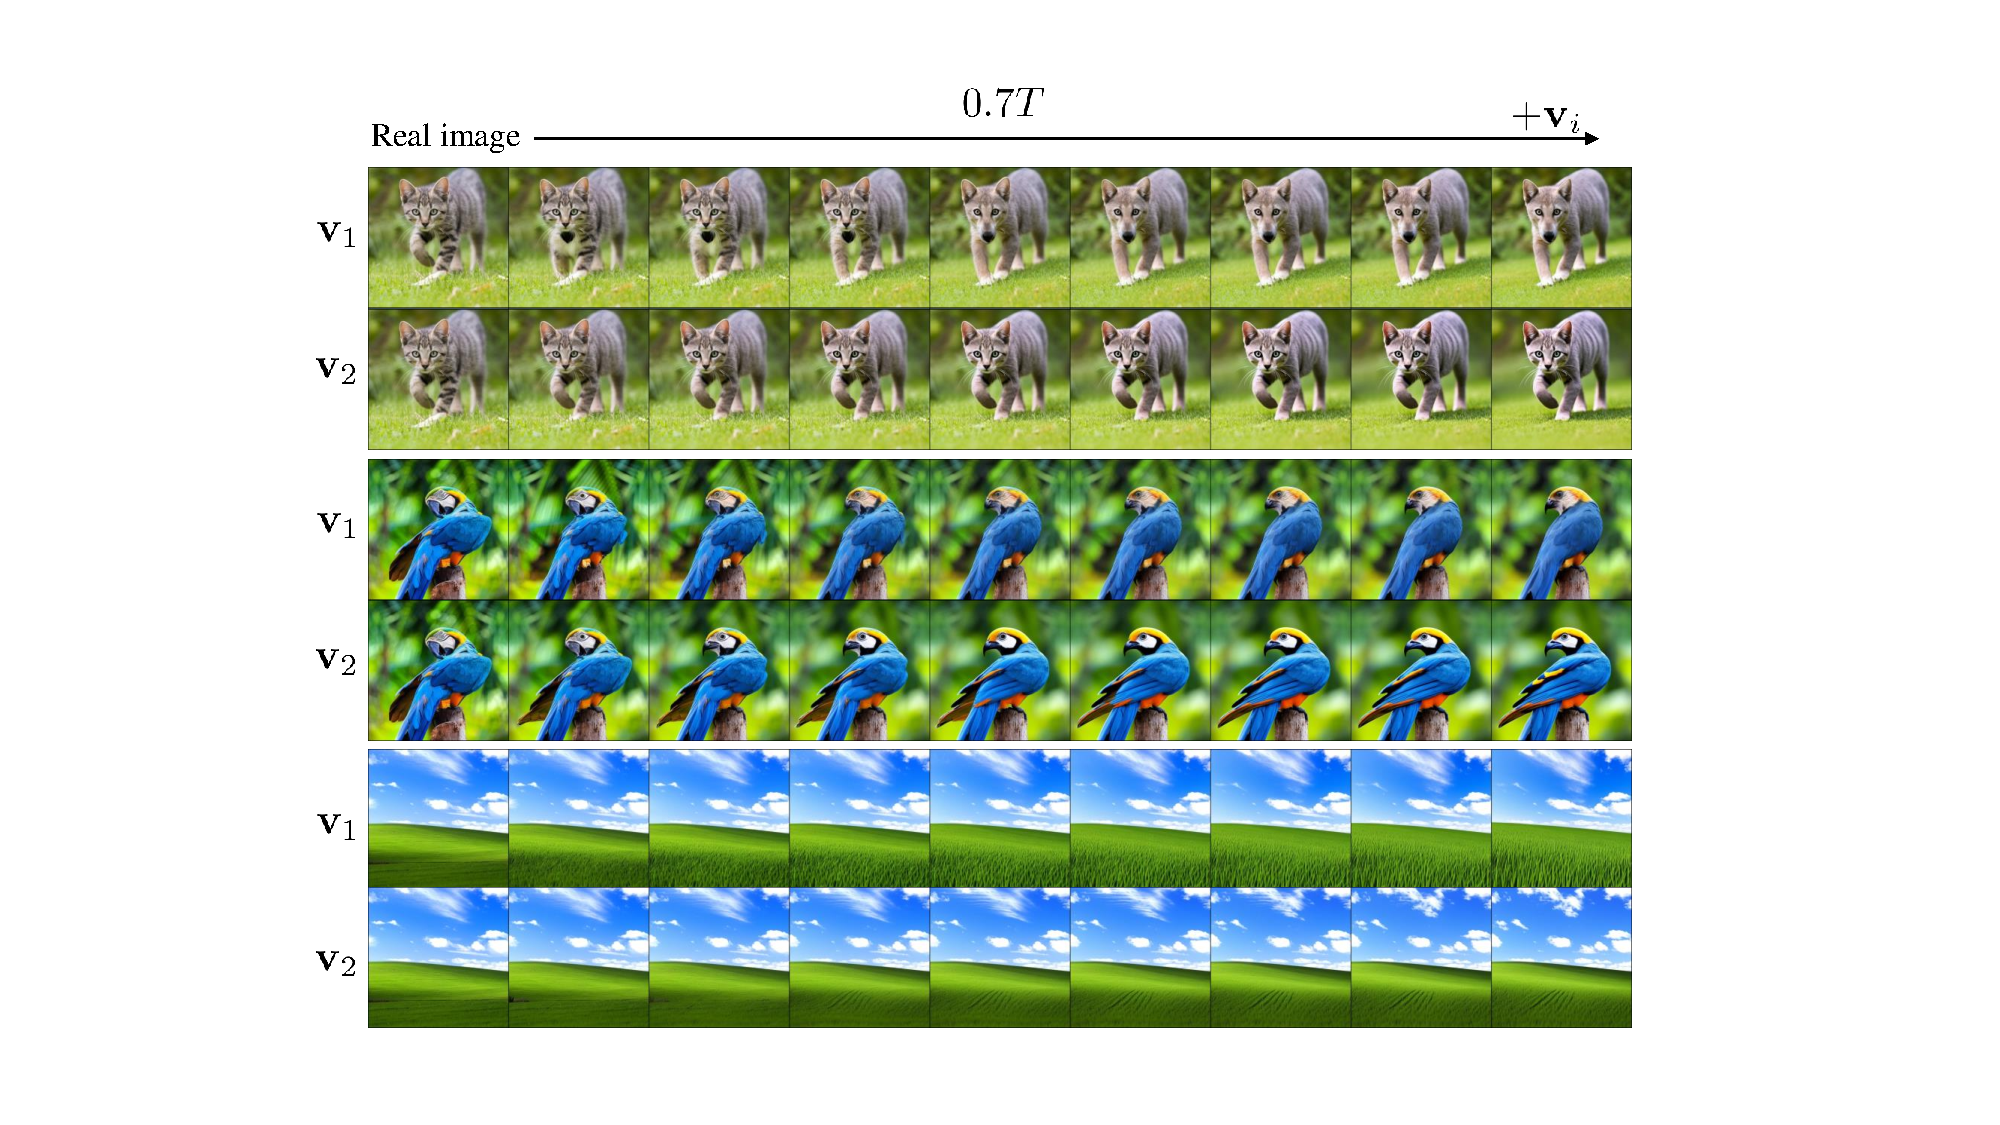
\includegraphics[width=1.0\linewidth]{figure/stable_7T.pdf}
    \caption{
    \textbf{More examples of image editing using the latent basis with Stable Diffusion.} The editing result using $\vv_i$' in Stable diffusion at 0.7$T$.}
    \label{fig:stable_7T}
\end{figure}

\clearpage

\begin{figure}[!h]
    \centering
    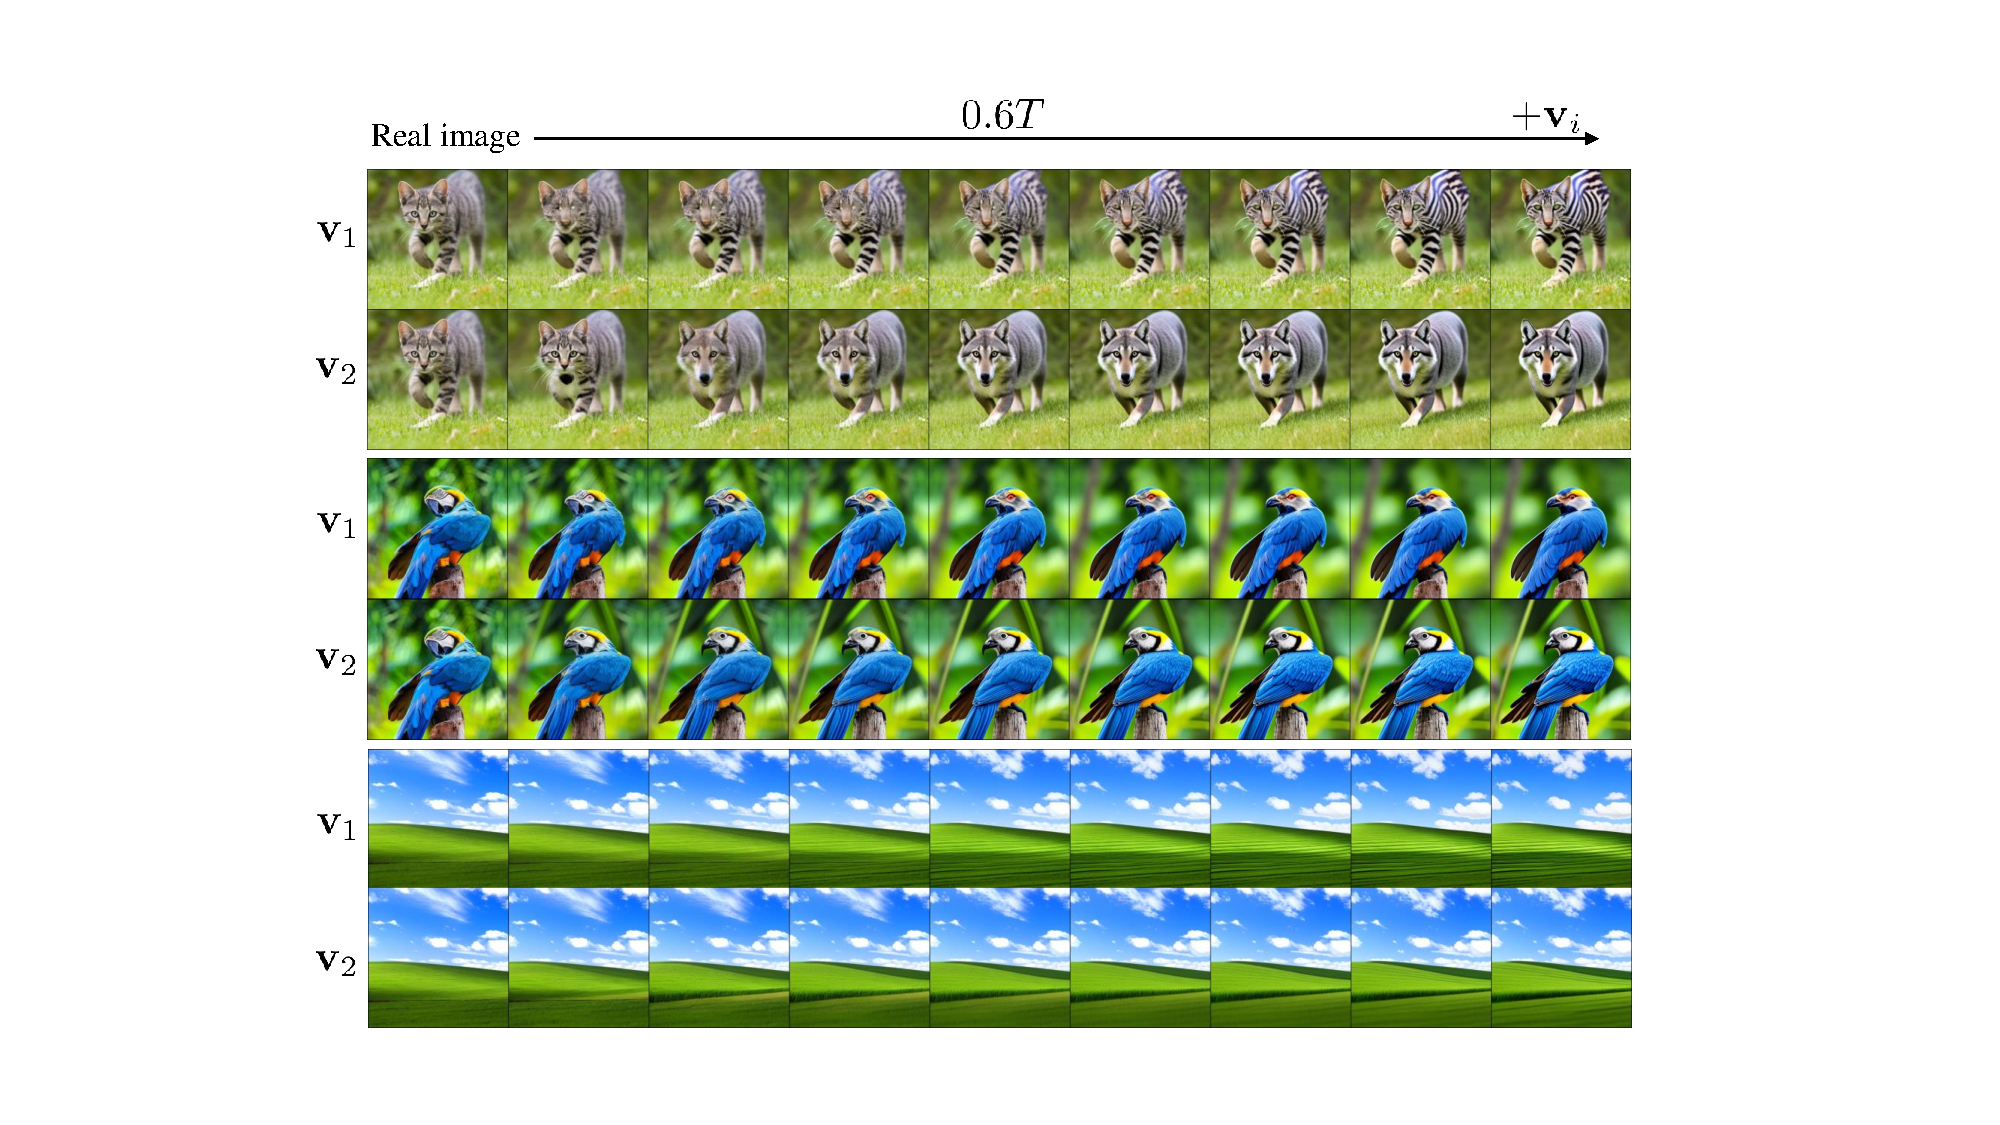
\includegraphics[width=1.0\linewidth]{figure/stable_6T.pdf}
    \caption{
    \textbf{More examples of image editing using the latent basis with Stable Diffusion.} The editing result using $\vv_i$' in Stable diffusion at 0.6$T$.}
    \label{fig:stable_6T}
\end{figure}


\paragraph{latent basis with given prompt}
%As shown in \fref{fig:stable_various_vis}, using the prompt as a condition, the entire latent basis captures prompt-related attributes. 
As shown in \fref{fig:stable_various_vis}, when we condition a specific prompt, such as ``Zebra'' or ``Chimpanzee'', the entire latent basis corresponds to the prompt-related attributes.
Notably, Changes to ``zebra'', which are clear, all show similar results, but ``chimpanzee'' show different results. Nevertheless, it is clear that they are all related to ``chimpanzee''.

 

\begin{figure}[!h]
    \centering
    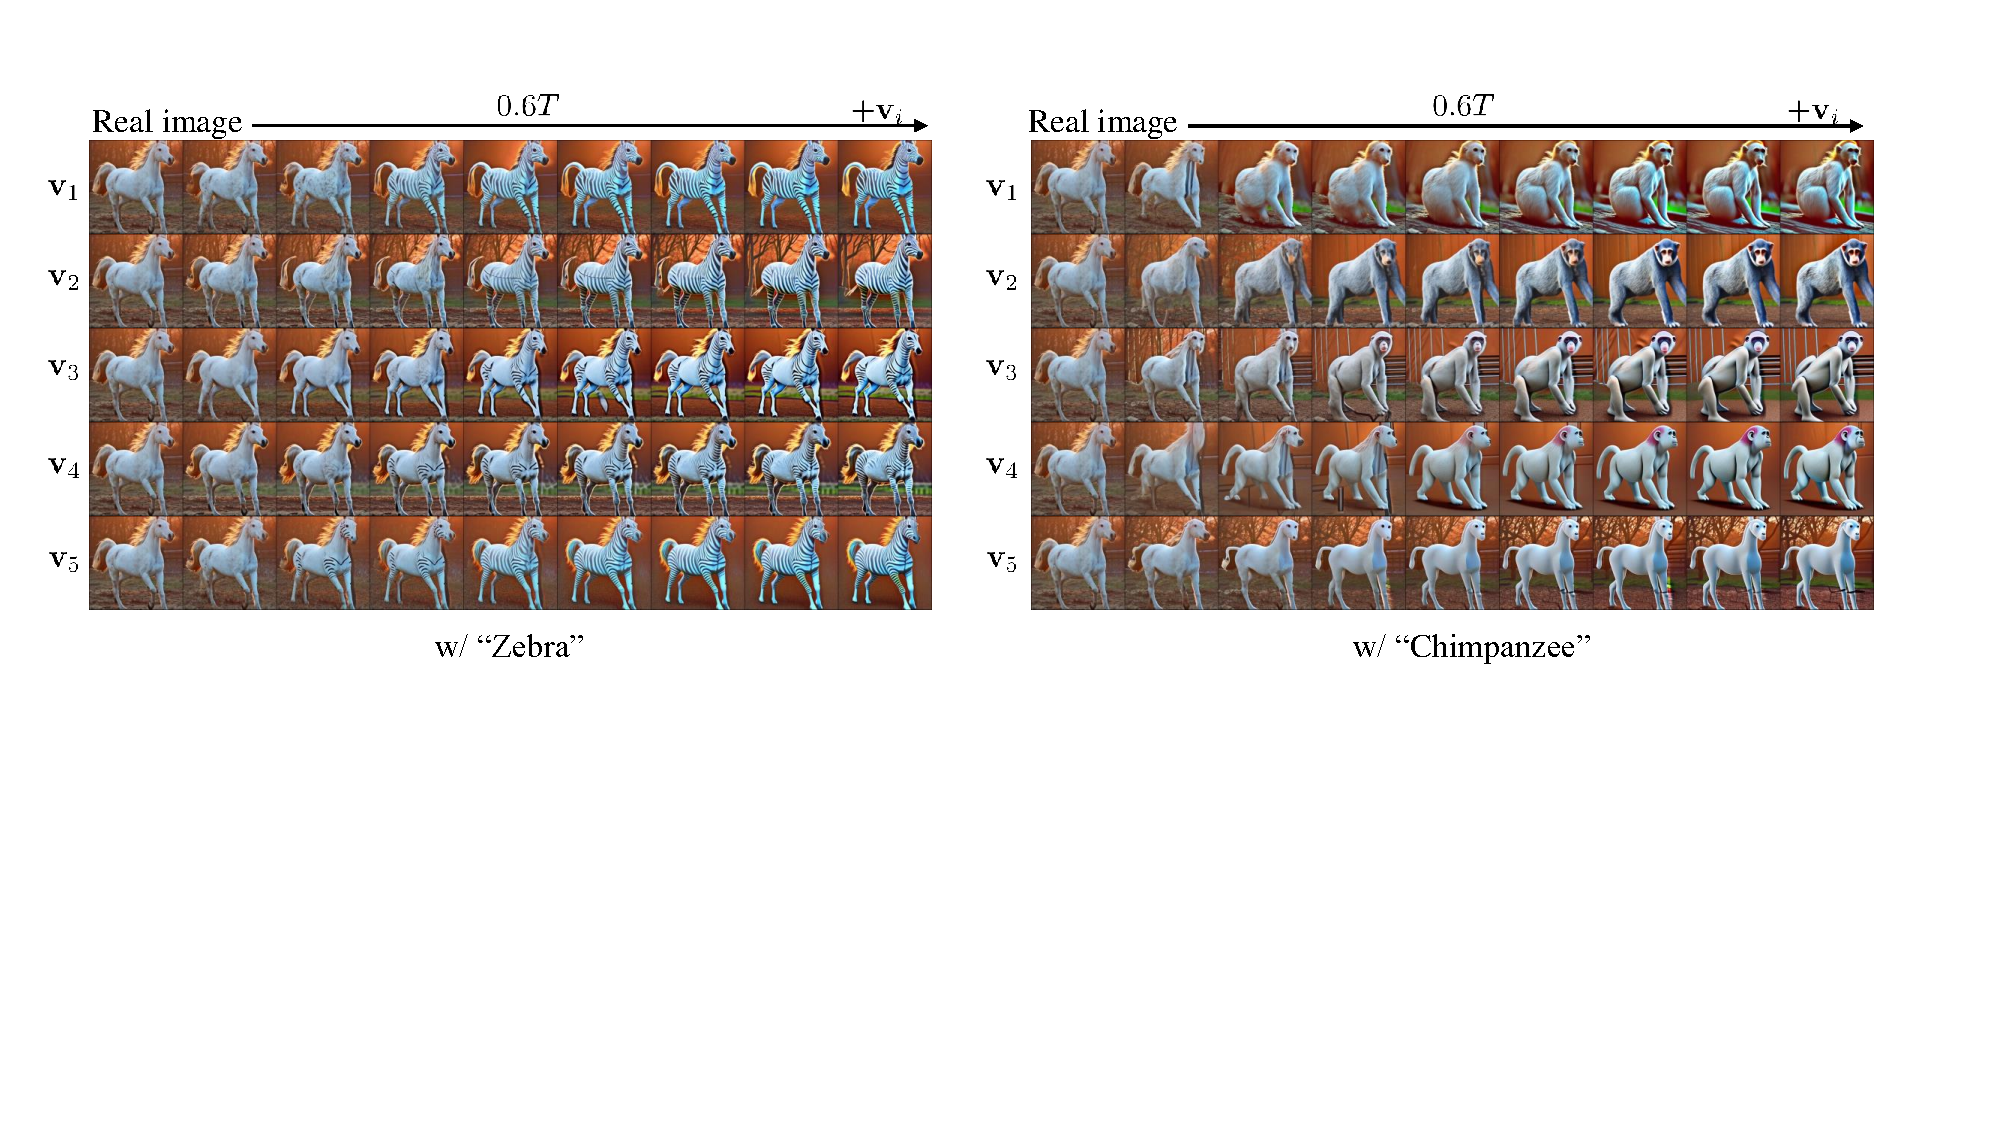
\includegraphics[width=1.0\linewidth]{figure/stable_various_vis.pdf}
    \vspace{-2em}
    \caption{
    \textbf{More examples of image editing using top-5 latent basis vectors when given the prompt.} Notably, Changes to ``zebras'', which are clear, all show similar results, but ``chimpanzees'' show different results. Nevertheless, it is clear that it is all related to ``chimpanzees''.}
    \label{fig:stable_various_vis}
\end{figure}


% \subsection{}
\subsection{Image editing using latent basis vectors discovered with various prompts}

We provide additional examples of image editing using latent basis vectors discovered with various prompts. \fref{fig:stable_text_more}, \ref{fig:stable_text_more2} show image editing with various pictures and various prompts. 
%The prompt of ``[···cat··]'' is ``a cat dressed as a witch wearing a wizard hat in a haunted house''. 
For brevity, we denote the prompt "a cat dressed as a witch wearing a wizard hat in a haunted house" by "[···cat··]" in \fref{fig:stable_text_more}.

\begin{figure}[!h]
    \centering
    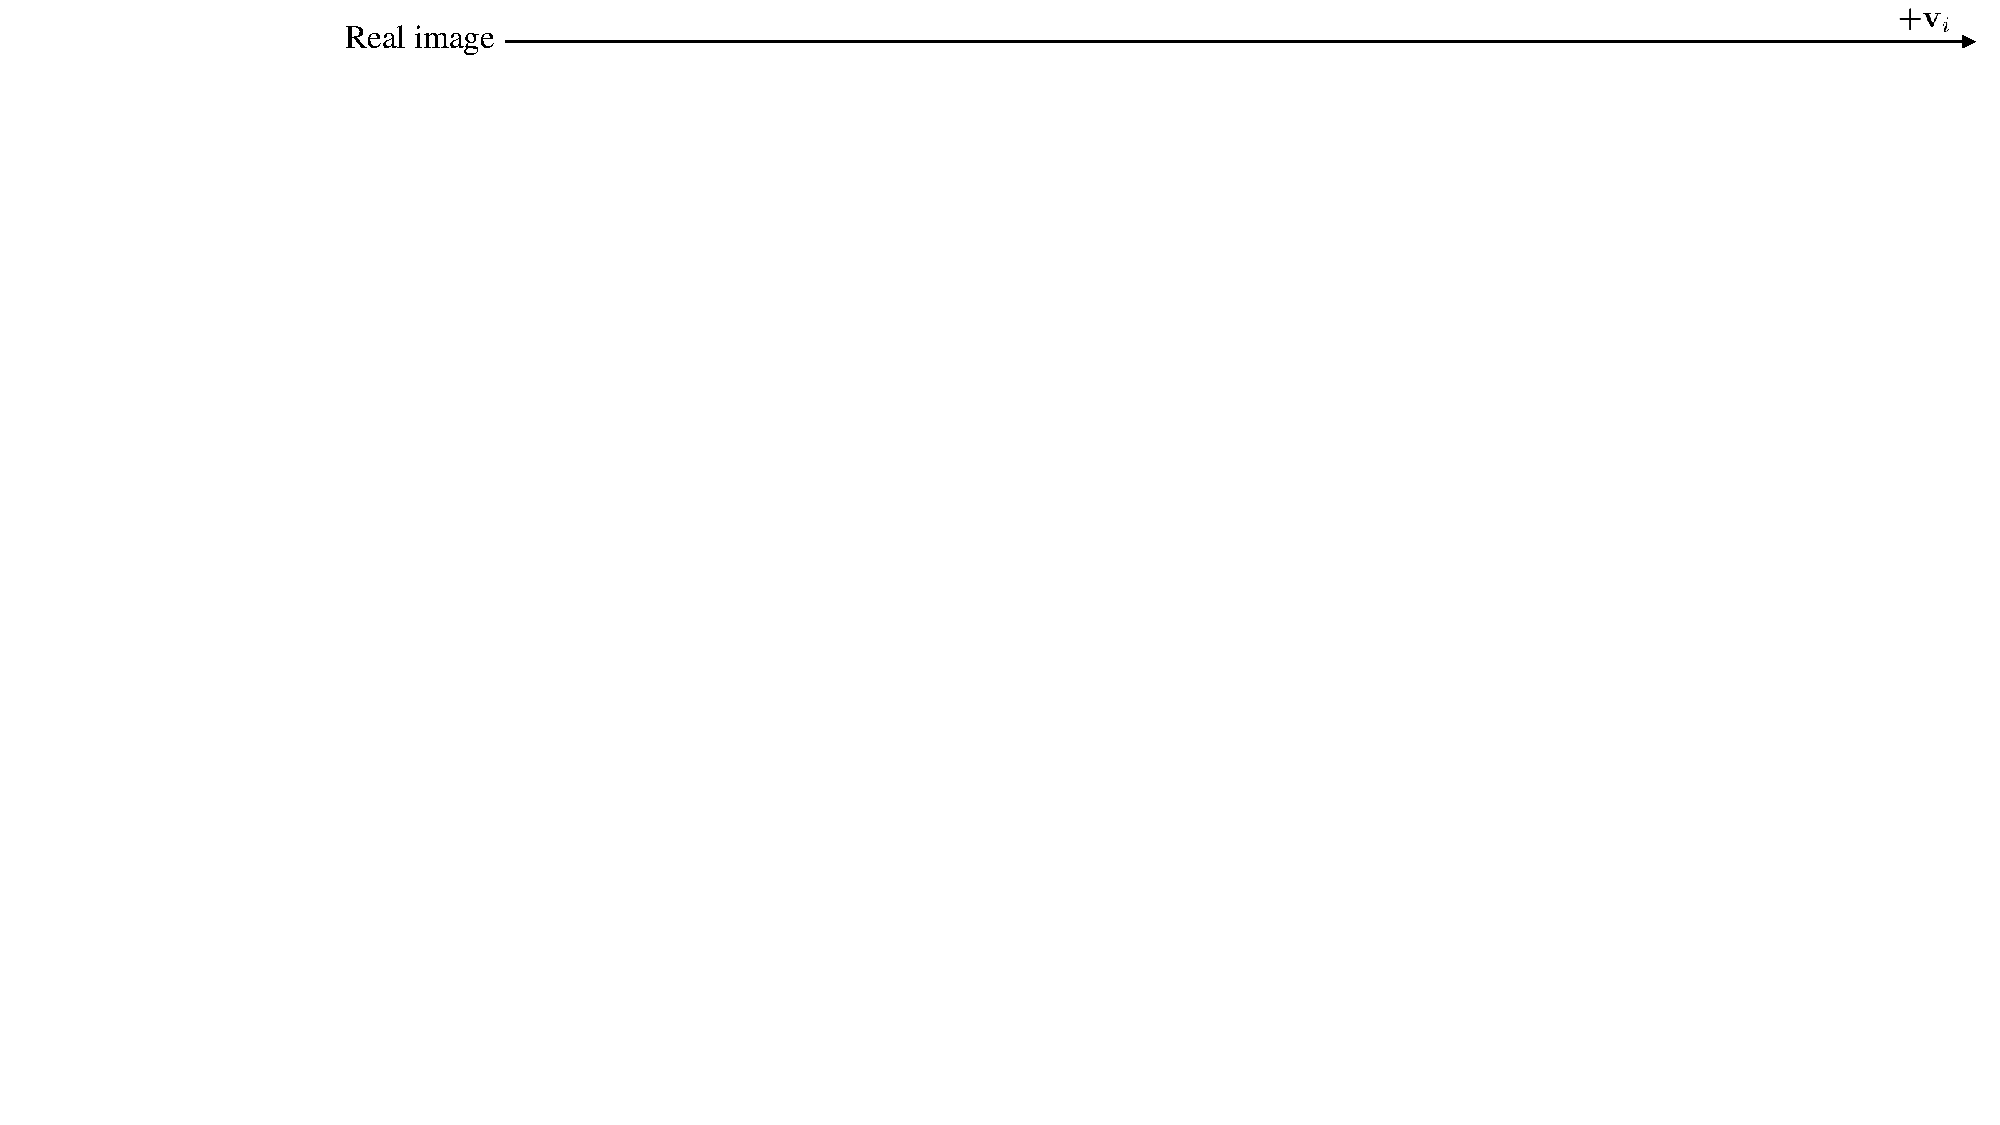
\includegraphics[width=1.0\linewidth]{figure/top.pdf}
    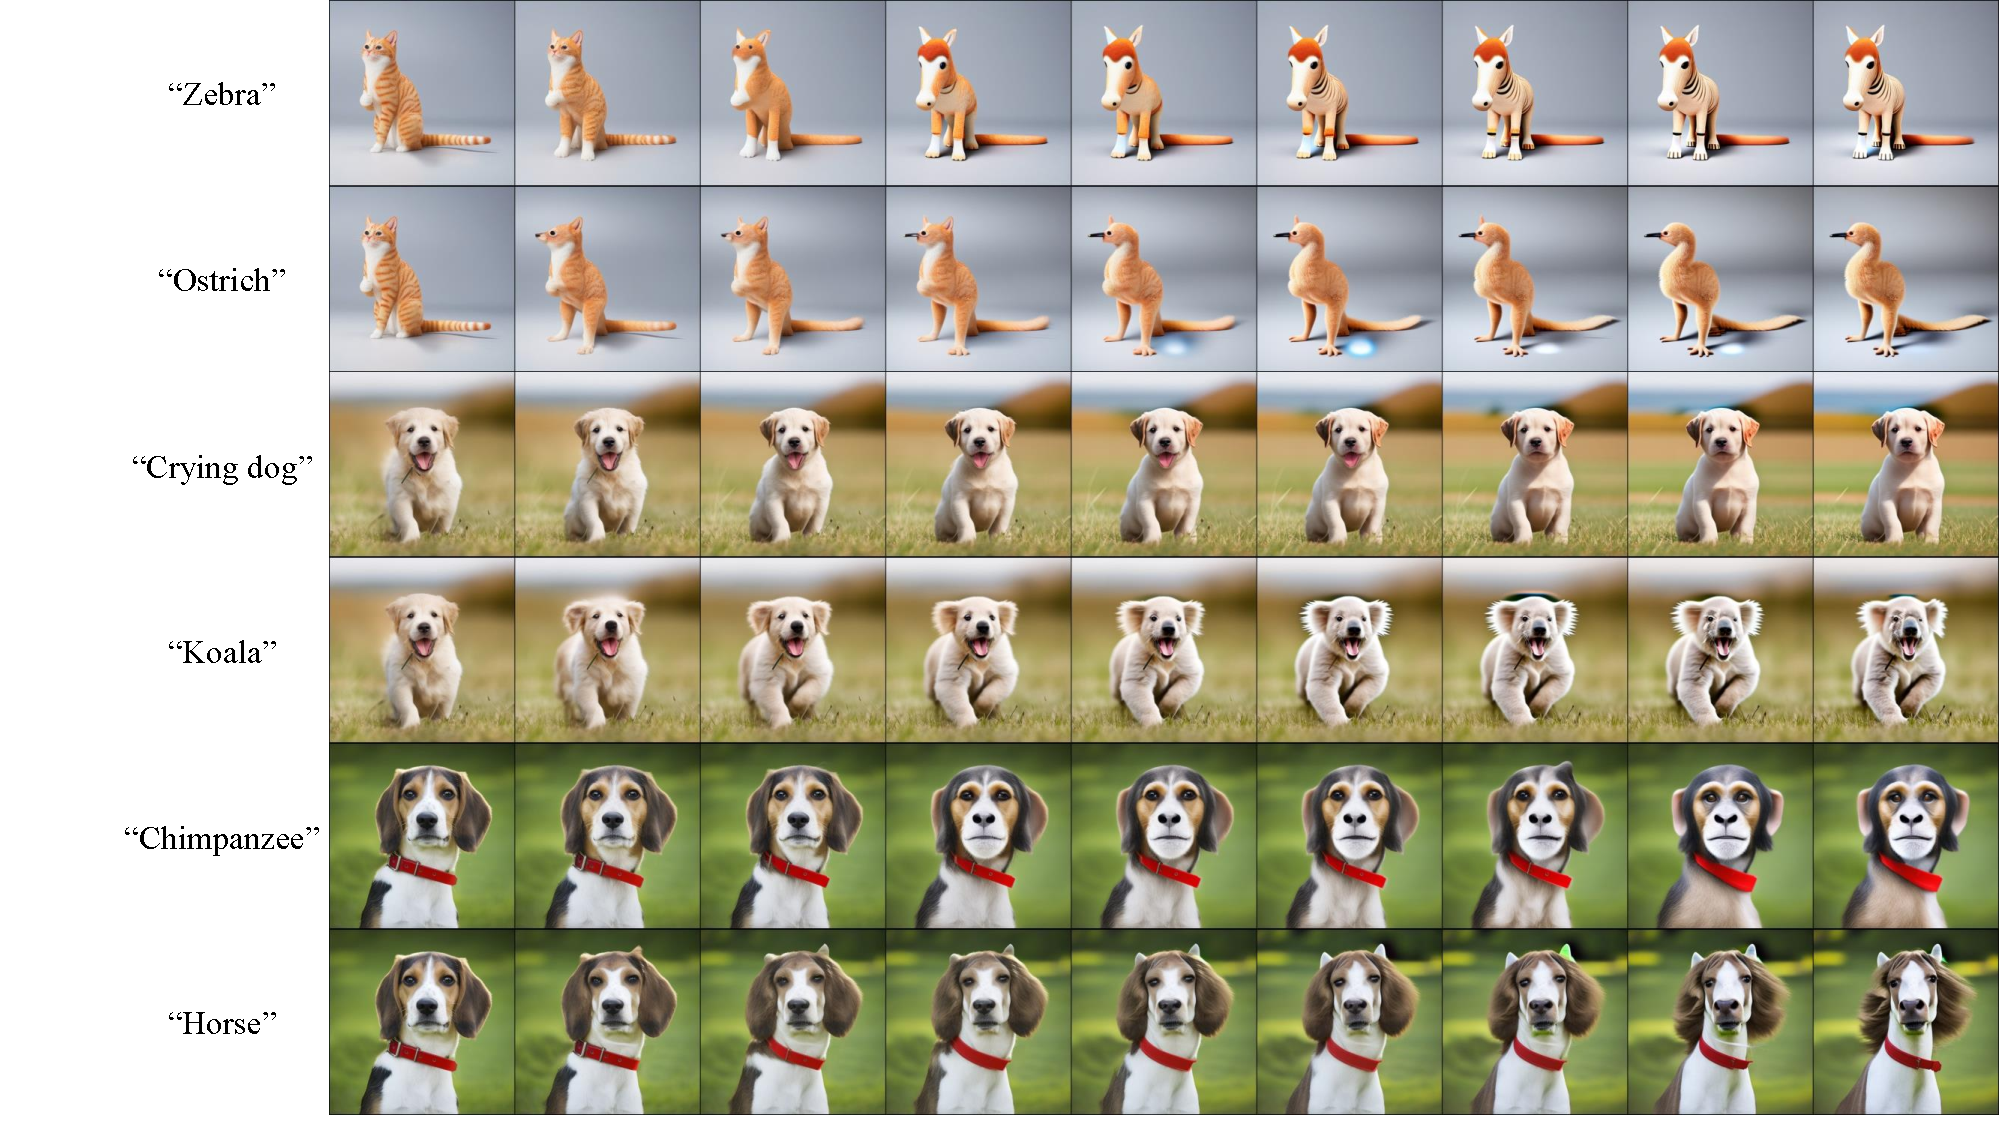
\includegraphics[width=1.0\linewidth]{figure/stable_text_1.pdf}
    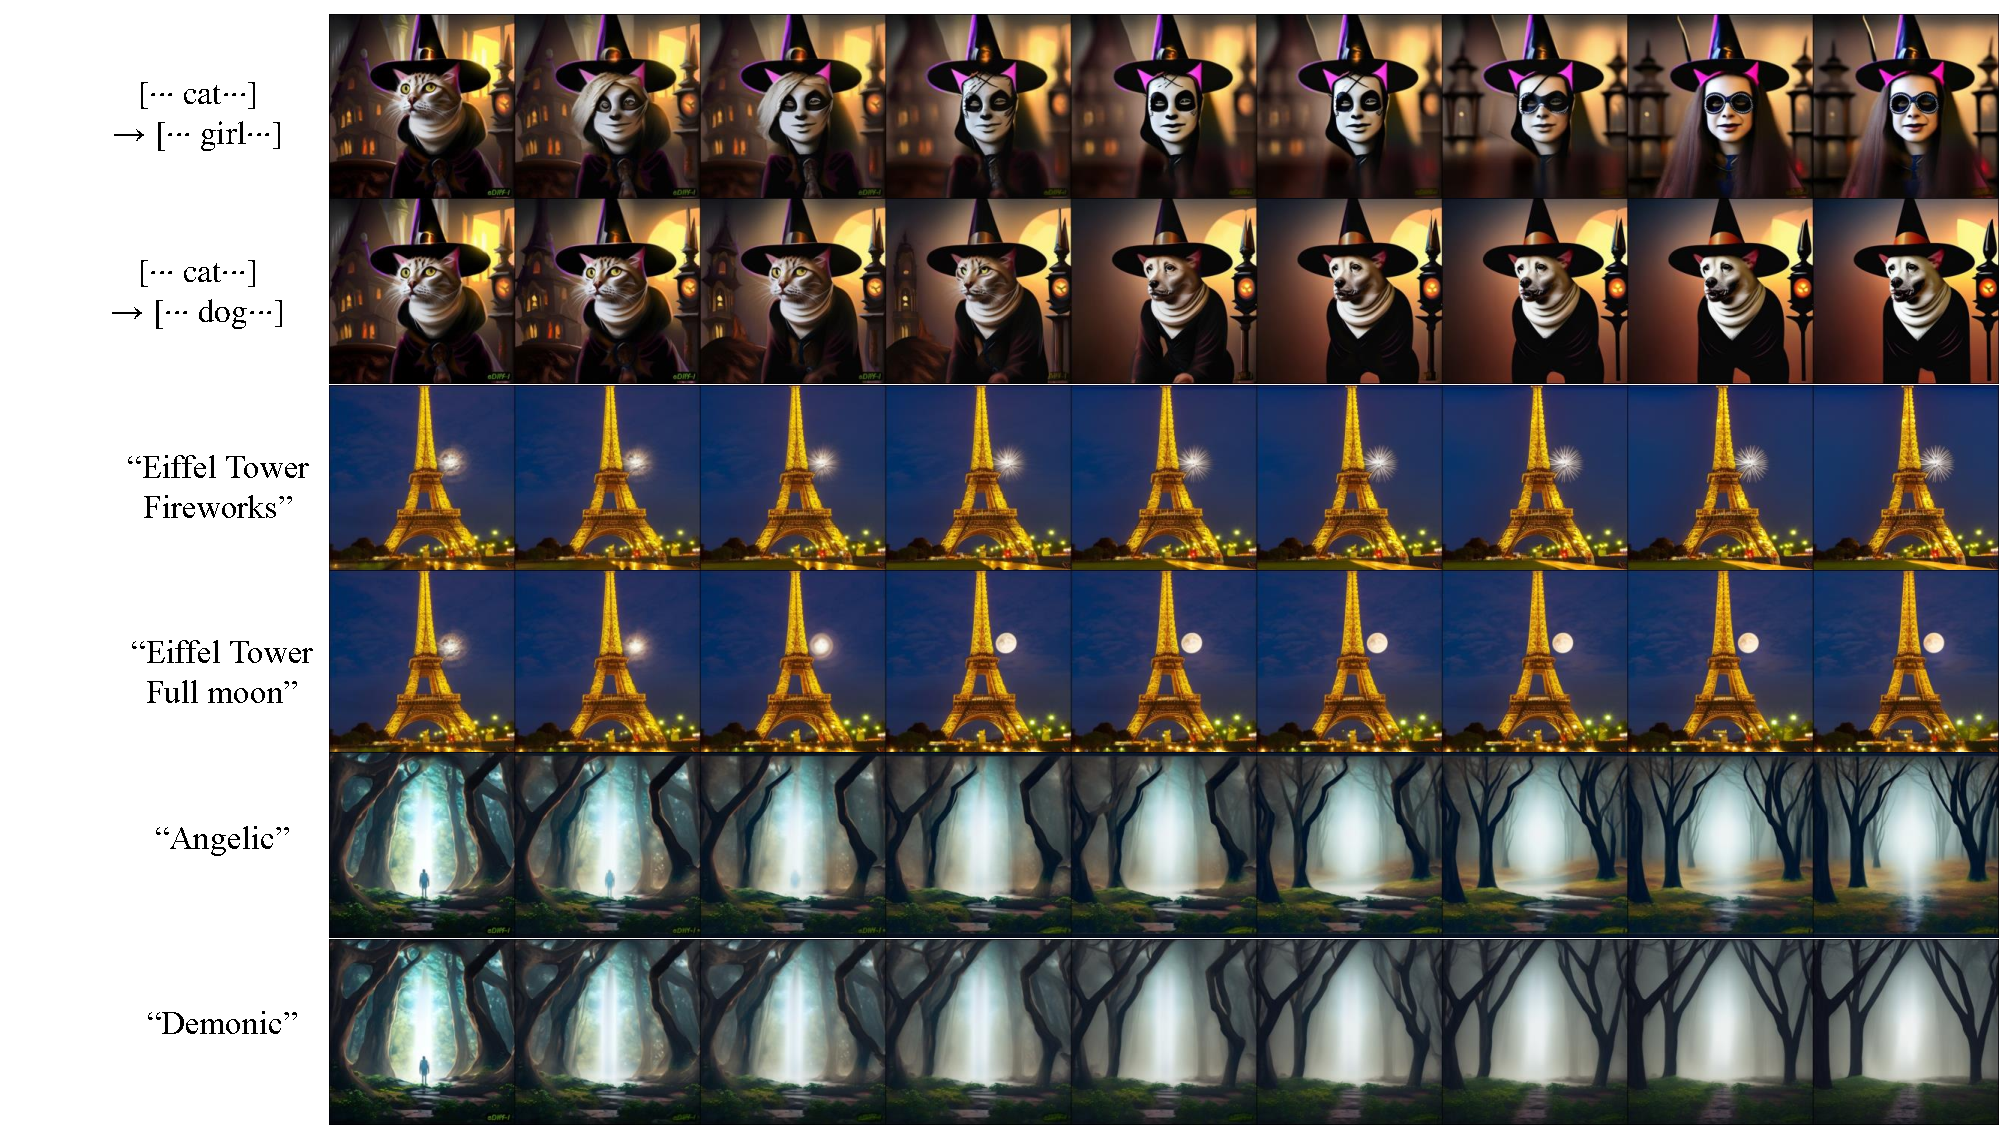
\includegraphics[width=1.0\linewidth]{figure/stable_text_2.pdf}
    \caption{
    \textbf{More examples of image editing using latent basis vectors discovered with various prompts.} }
    \label{fig:stable_text_more}
\end{figure}

\clearpage

\begin{figure}[!h]
    \centering
    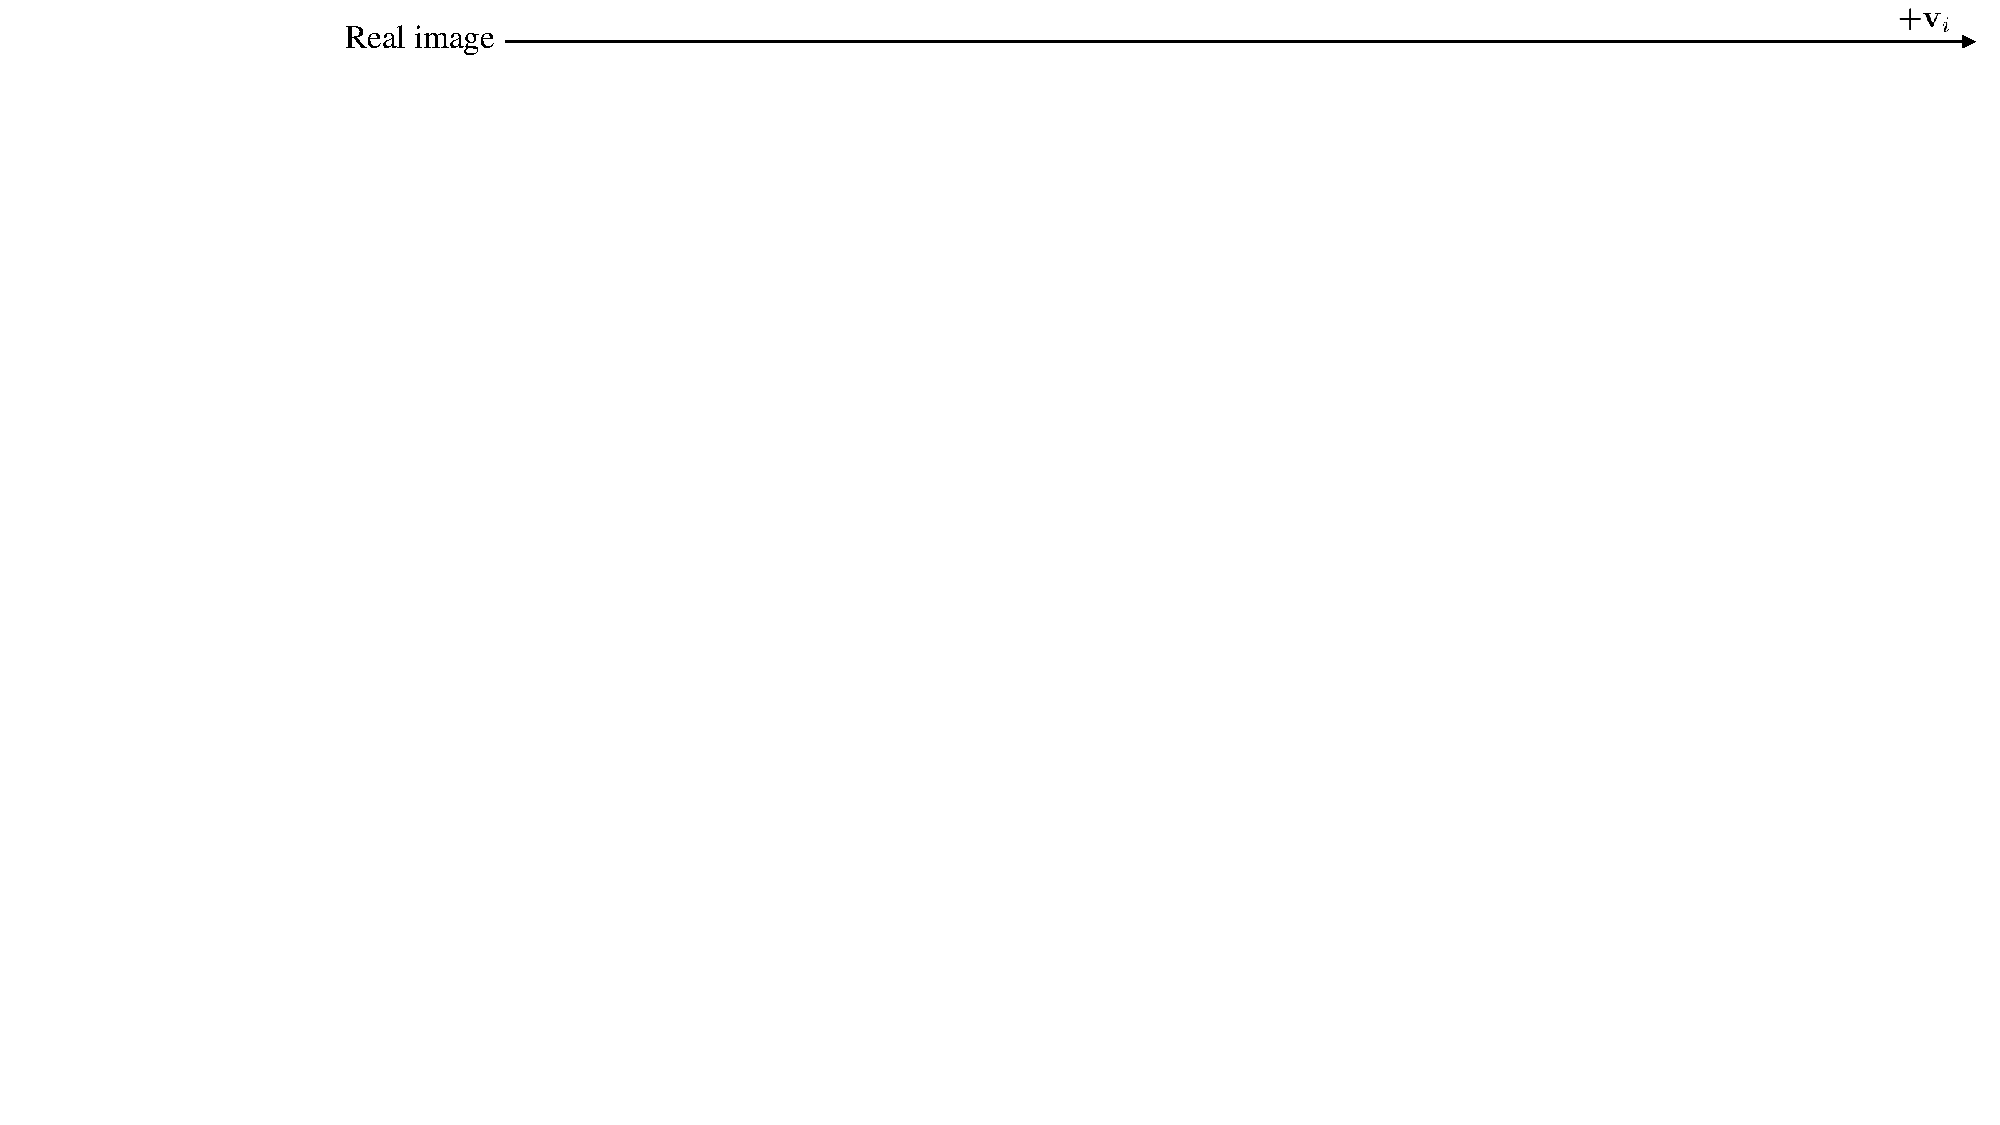
\includegraphics[width=1.0\linewidth]{figure/top.pdf}
    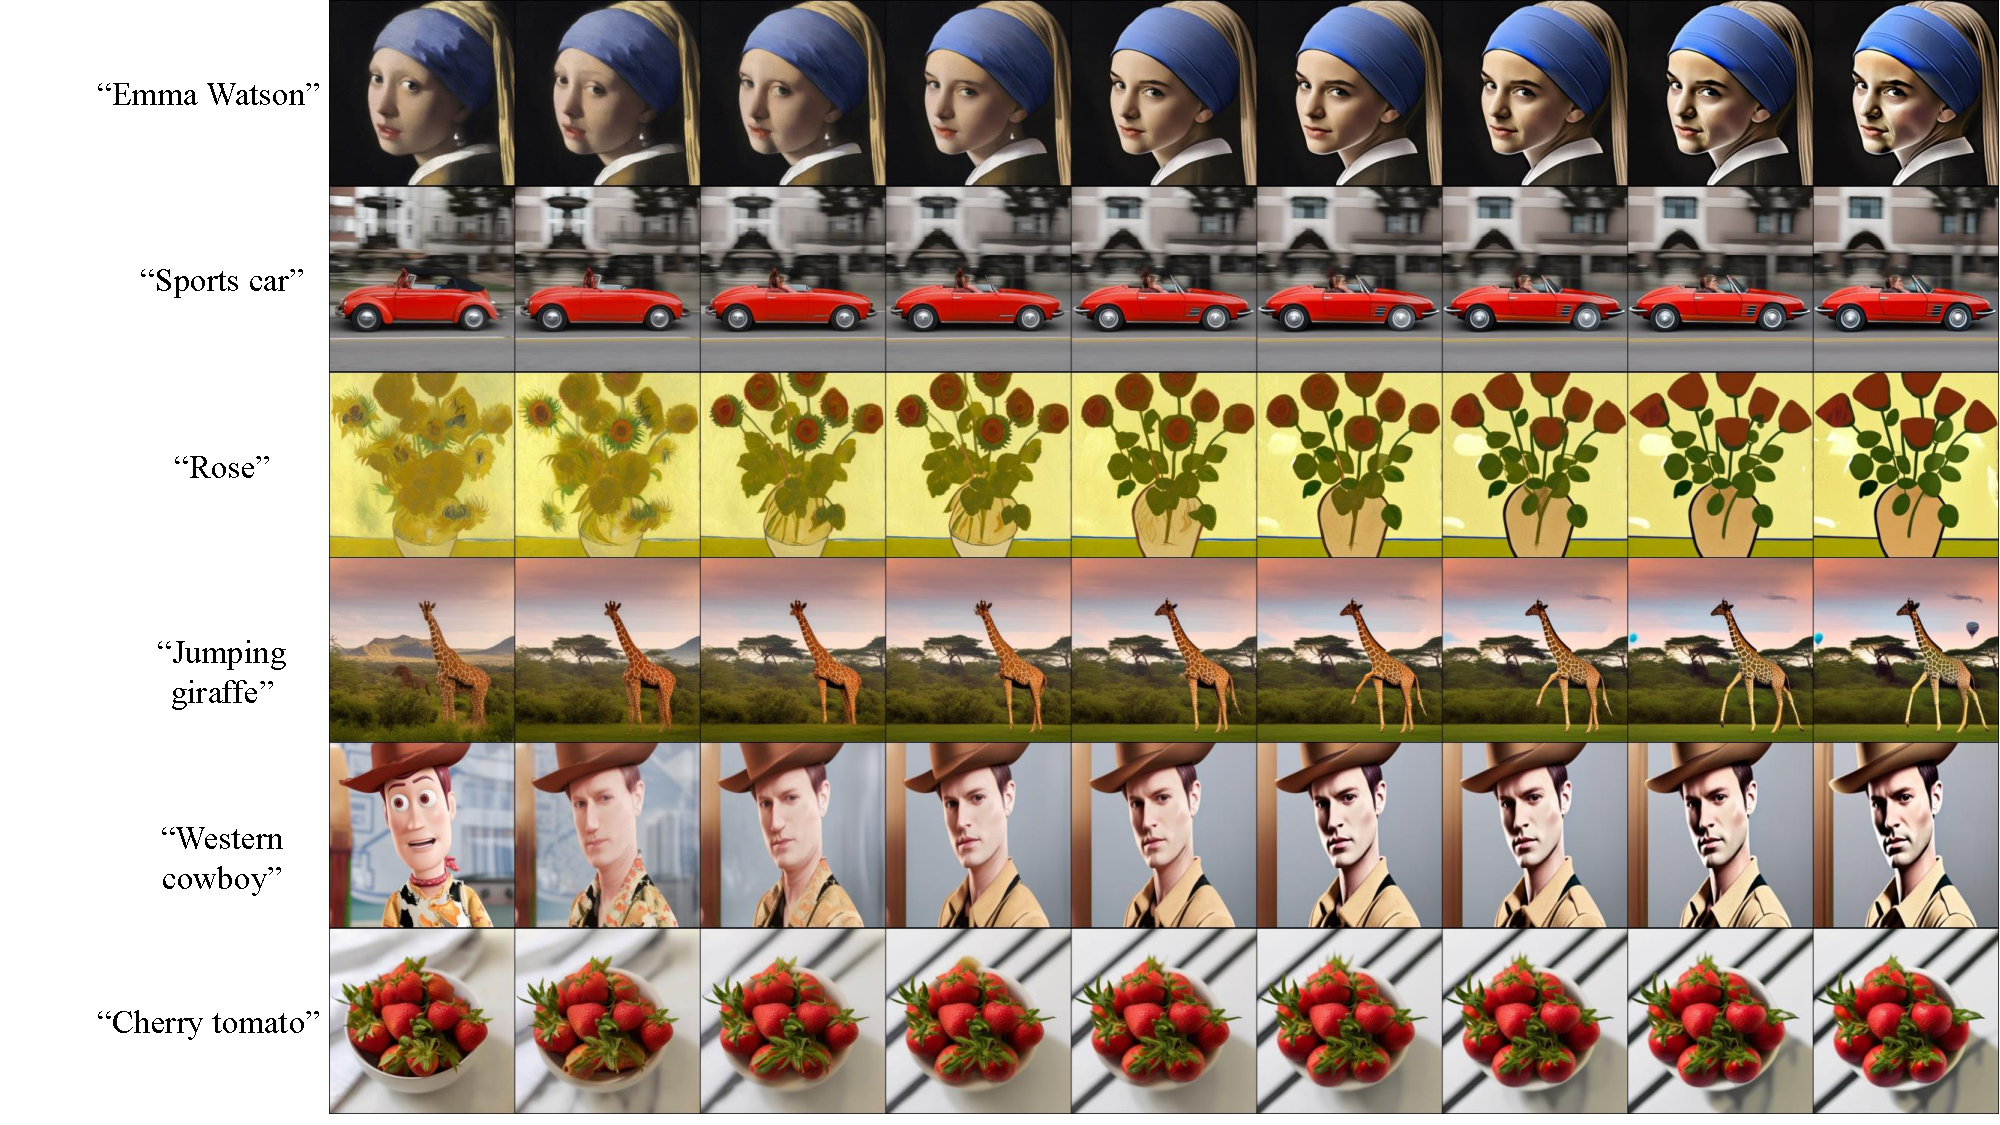
\includegraphics[width=1.0\linewidth]{figure/stable_text_3.pdf}
    \caption{
    \textbf{More examples of image editing using latent basis vectors discovered with various prompts.} }
    \label{fig:stable_text_more2}
\end{figure}

% \subsection{More discussion of using latent basis vectors discovered with various prompts}
\subsection{More discussion on the editing capability of the latent basis discovered with text conditions}
\label{appen:more_discussion}

In this subsection, we provide a discussion based on the failure cases of our approach. \fref{fig:stable_1T} shows the results of latent basis found at $t=T$ with Stable diffusion. Unlike unconditional models, the directions found at $t=T$ exhibit rapid and drastic unexpected changes. 
%However, it was observed that for landscape photos without a main object, the expected editing effects were demonstrated at any timesteps. 
However, landscape photos, which do not contain a main object, exhibited desired editing effects at any timesteps.
Moreover, in the case of landscapes, it is conjectured that the latent basis plays a significant role in representing patterns and textures. 
Analyzing the landscape images generated by Stable diffusion would be an interesting topic.

\fref{fig:more_limitations} presents examples of failure cases in our image editing using latent basis vectors discovered with various prompts.
(a) When using pose or action as a prompt, there are instances where the identity is not preserved.
(b) When the shape of the target subject differs significantly from the source image, the results are often unsatisfactory.
(c) There are cases where the preservation of the background is not achieved.
(d) It is challenging to make significant changes to the entire image.

Regarding the reasons for these failure cases, we emphasize two factors.
First, we manipulate in the \exspace{}. % ``$\vx_t$''. 
% We adopt a direct manipulation of $\vx_t$ to analyze the latent space of the diffusion model. 
The result in \fref{fig:more_limitations} (a) implies that \exspace{} is not a space where disentanglement for identity is achieved effectively.
On the other hand, in \ehspace{}, there are results indicating successful preservation of identity \cite{kwon2022diffusion, haas2023discovering}. 
Investigating the disentanglement capability of \exspace{} and any other distinguishing features it may have compared to \ehspace{} would be an interesting future research topic.

Secondly, we perform manipulation by adding and subtracting the "signal" that the model pays attention to in $\vx_t$.
% The directions we find represent the signal captured by the model's features. 
Here, The signal is captured from the current input $\vx_t$, which limits the deviation from the original form. Therefore, when there is a substantial difference in shape, such as transforming a giraffe into a tiger, the results may not be satisfactory. (\fref{fig:more_limitations} (b))
When we utilize text conditions, the latent basis aligns with the text information. This leads to not capturing background information, resulting in changes in the background when manipulated. It is also an interesting research topic to capture signals related to the background. (\fref{fig:more_limitations} (c))
% Since we utilize the top $n$ signals captured by the features, they often do not include background information. It is also an interesting research topic to capture signals related to the background. (\fref{fig:more_limitations} (c))
Since the model focuses on finer features as t approaches 0, if broad changes are desired, manipulation should be performed at $t=T$. However, manipulation at $t=T$ is unstable. Deep analysis of $\vx_t$ at $t=T$ in Stable diffusion is also an intriguing research topic. (\fref{fig:more_limitations} (d))

% Regarding the reasons for these failure cases, we emphasize two factors.
% First, the ``signal''. The directions we find represent the signal captured by the model's features. This signal is entirely determined by the given text, which can result in a loss of identity preservation. The signal is captured from the current input $\vx_t$, which limits the deviation from the original form. Therefore, when there is a substantial difference in shape, such as transforming a giraffe into a tiger, the results may not be satisfactory. Since we utilize the top $n$ signals captured by the features, they often do not include background information. It is also an interesting research topic to capture signals related to the background.

Despite these limitations, we have successfully achieved direct manipulation in the latent space $\vx_t$ at a single timestep, which, to our knowledge, is the first of its kind. Through this, we provide insights into the model and contribute to the understanding of the latent space, hopefully benefiting the diffusion community.

\begin{figure}[!h]
    \centering
    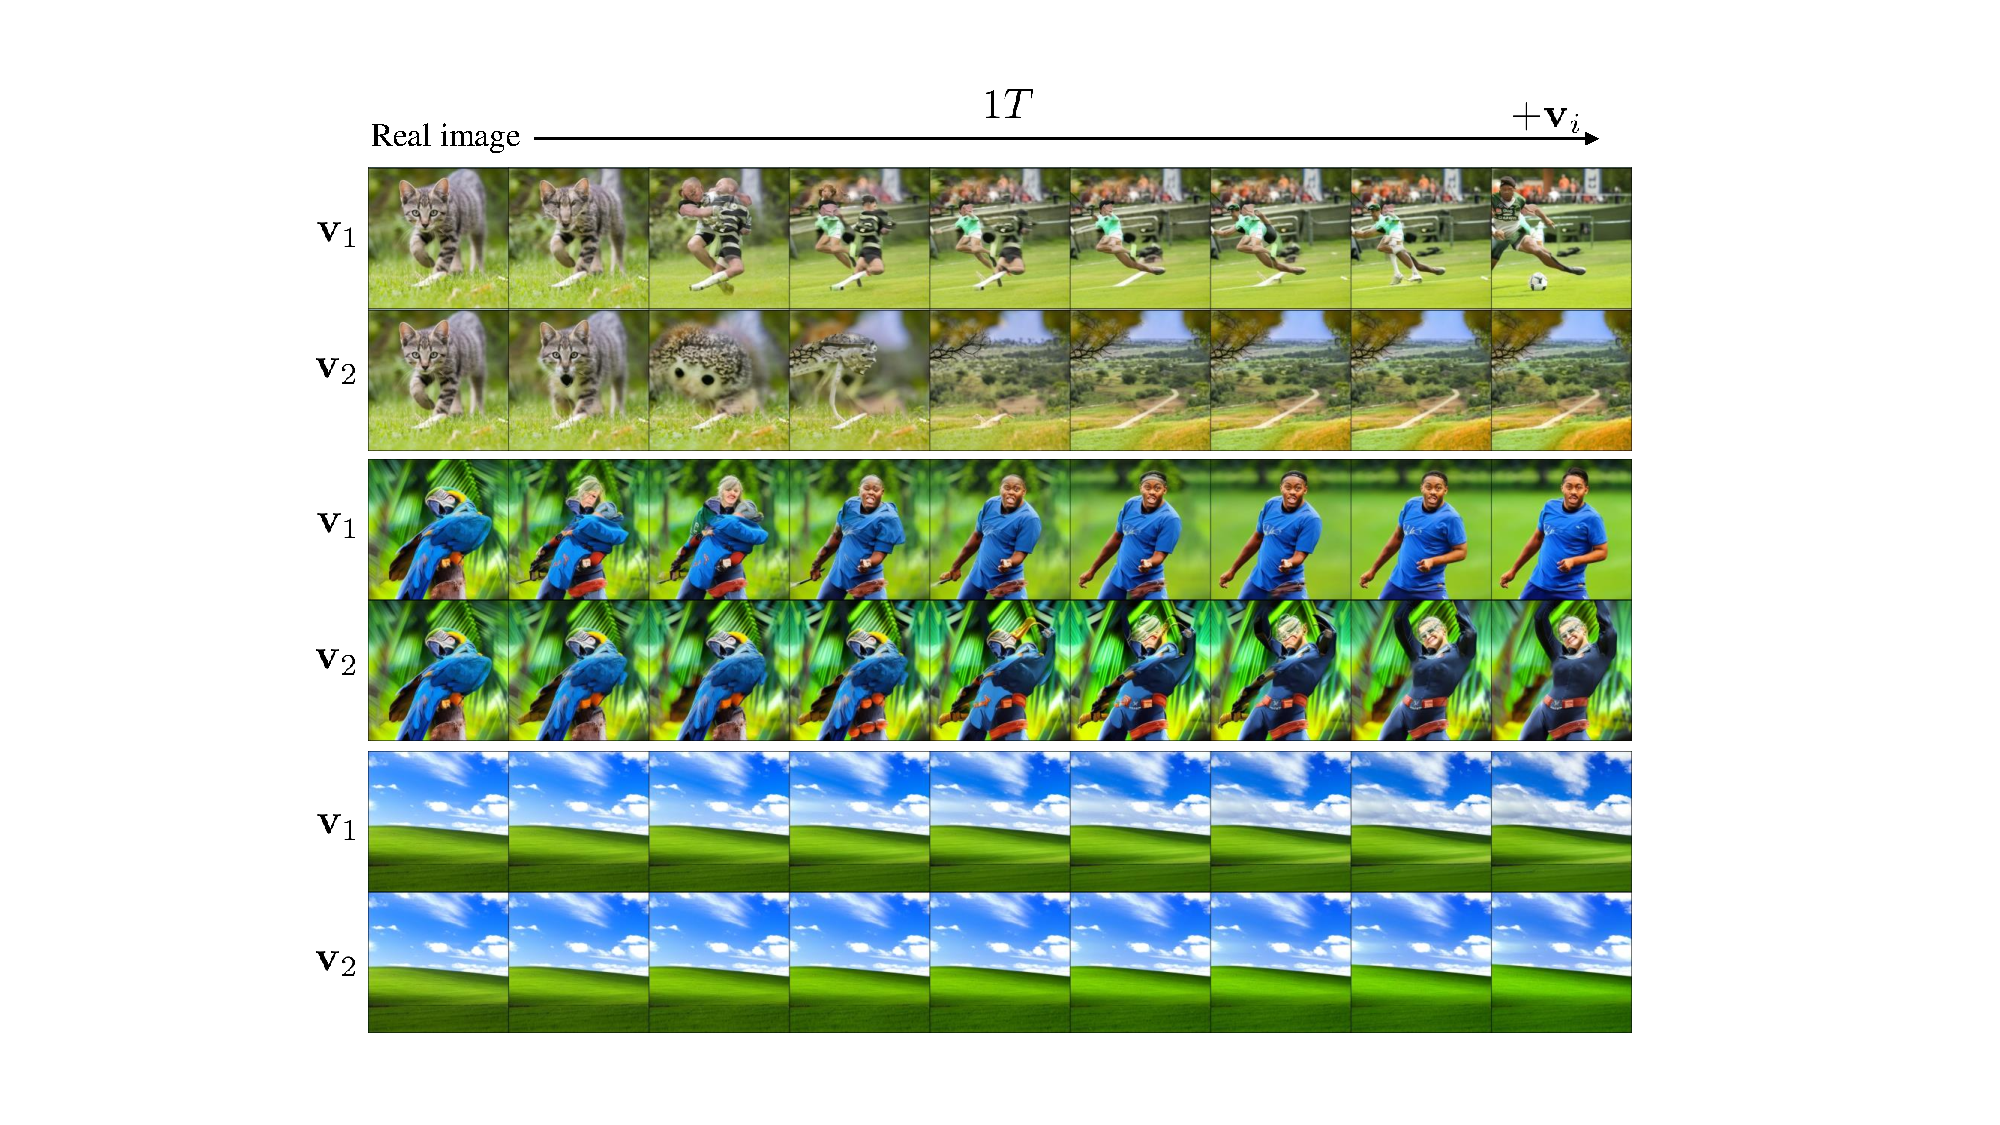
\includegraphics[width=0.8\linewidth]{figure/stable_1T.pdf}
    \caption{
    \textbf{Failure cases of image editing using the latent basis at 1$T$.} The editing result using $\vv_i$' in Stable diffusion at 1$T$.}
    \label{fig:stable_1T}
\end{figure}

\begin{figure}[!h]
    \centering
    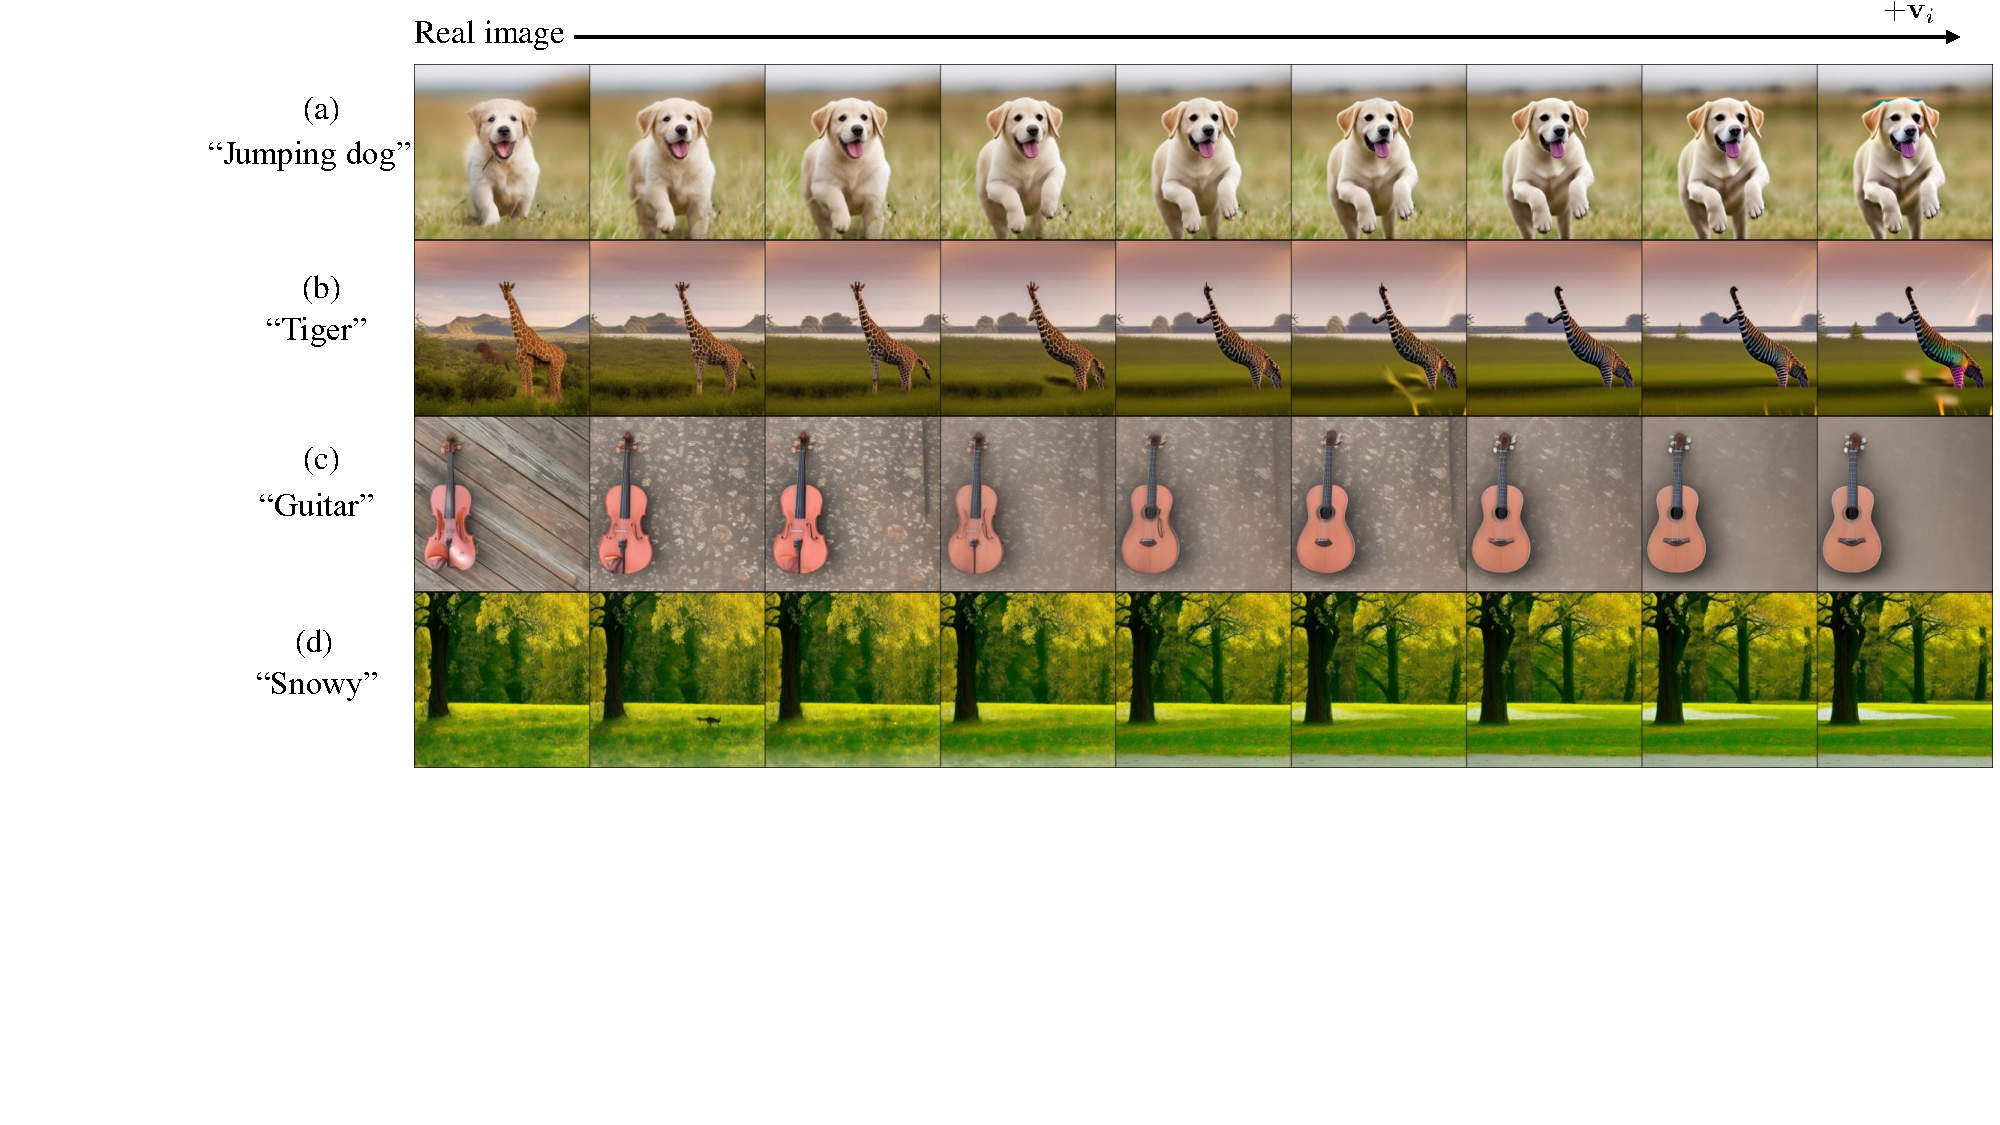
\includegraphics[width=1.0\linewidth]{figure/more_limitations.pdf}
    \caption{
    \textbf{Failure cases of using prompts.} (a) When using pose or action as a prompt, there are instances where the identity is not preserved.
(b) When the shape of the target subject differs significantly from the source image, the results are often unsatisfactory.
(c) There are cases where the preservation of the background is not achieved.
(d) It is challenging to make significant changes to the entire image.}
    \label{fig:more_limitations}
\end{figure}

% \begin{figure}[!t]
%     \centering
%     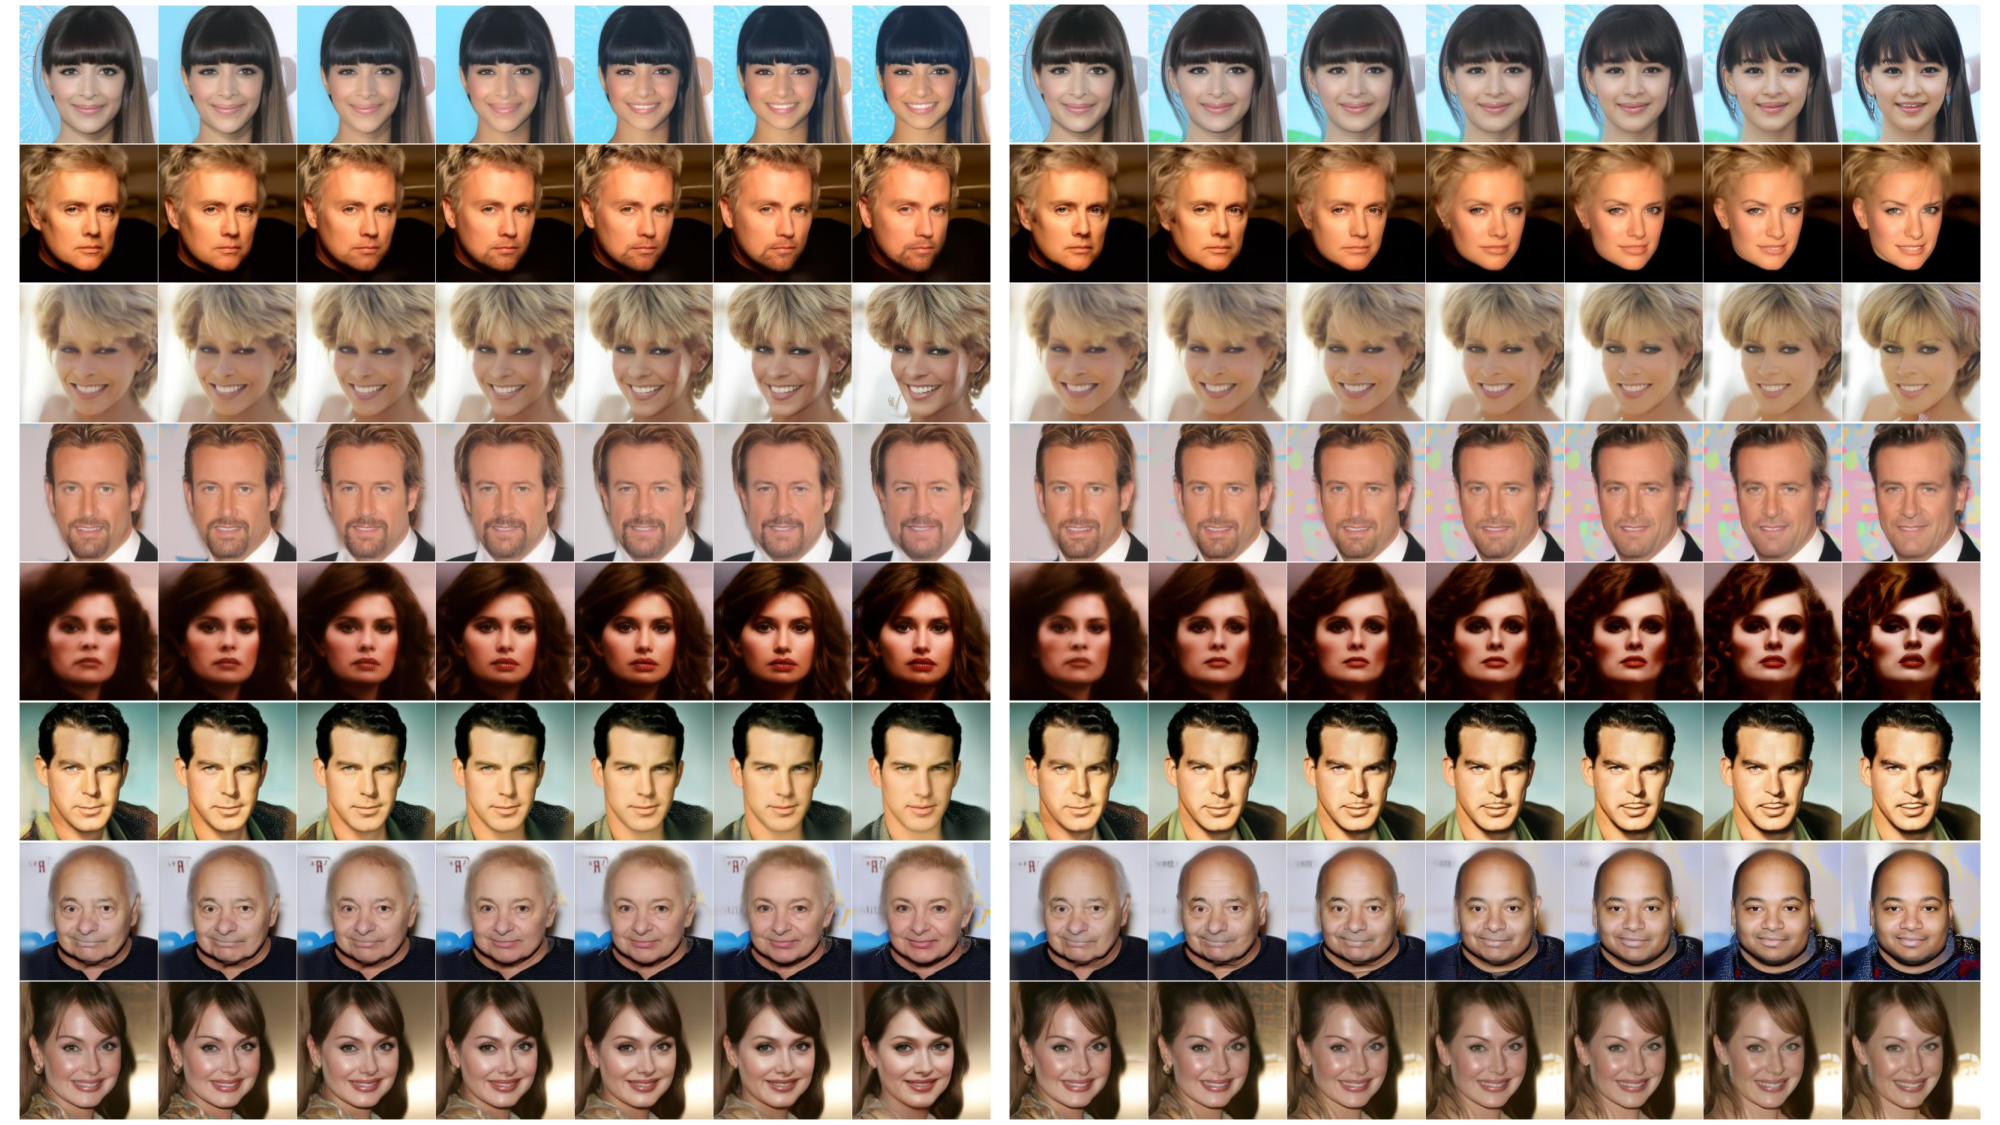
\includegraphics[width=1.0\linewidth]{figure/celeba_local_appendix_75.pdf}
%     \caption{
%     \textbf{$\boldsymbol{t=0.75T}$.} A selection of interpretable edits discovered by our feature direction in CelebA-HQ. The image on the far left represents the reconstructed original image, while the subsequent images demonstrate the interpretable edits that have been made to it.}
%     \label{fig:celeba_local_appendix_75}
% \end{figure}

% \begin{figure}[!t]
%     \centering
%     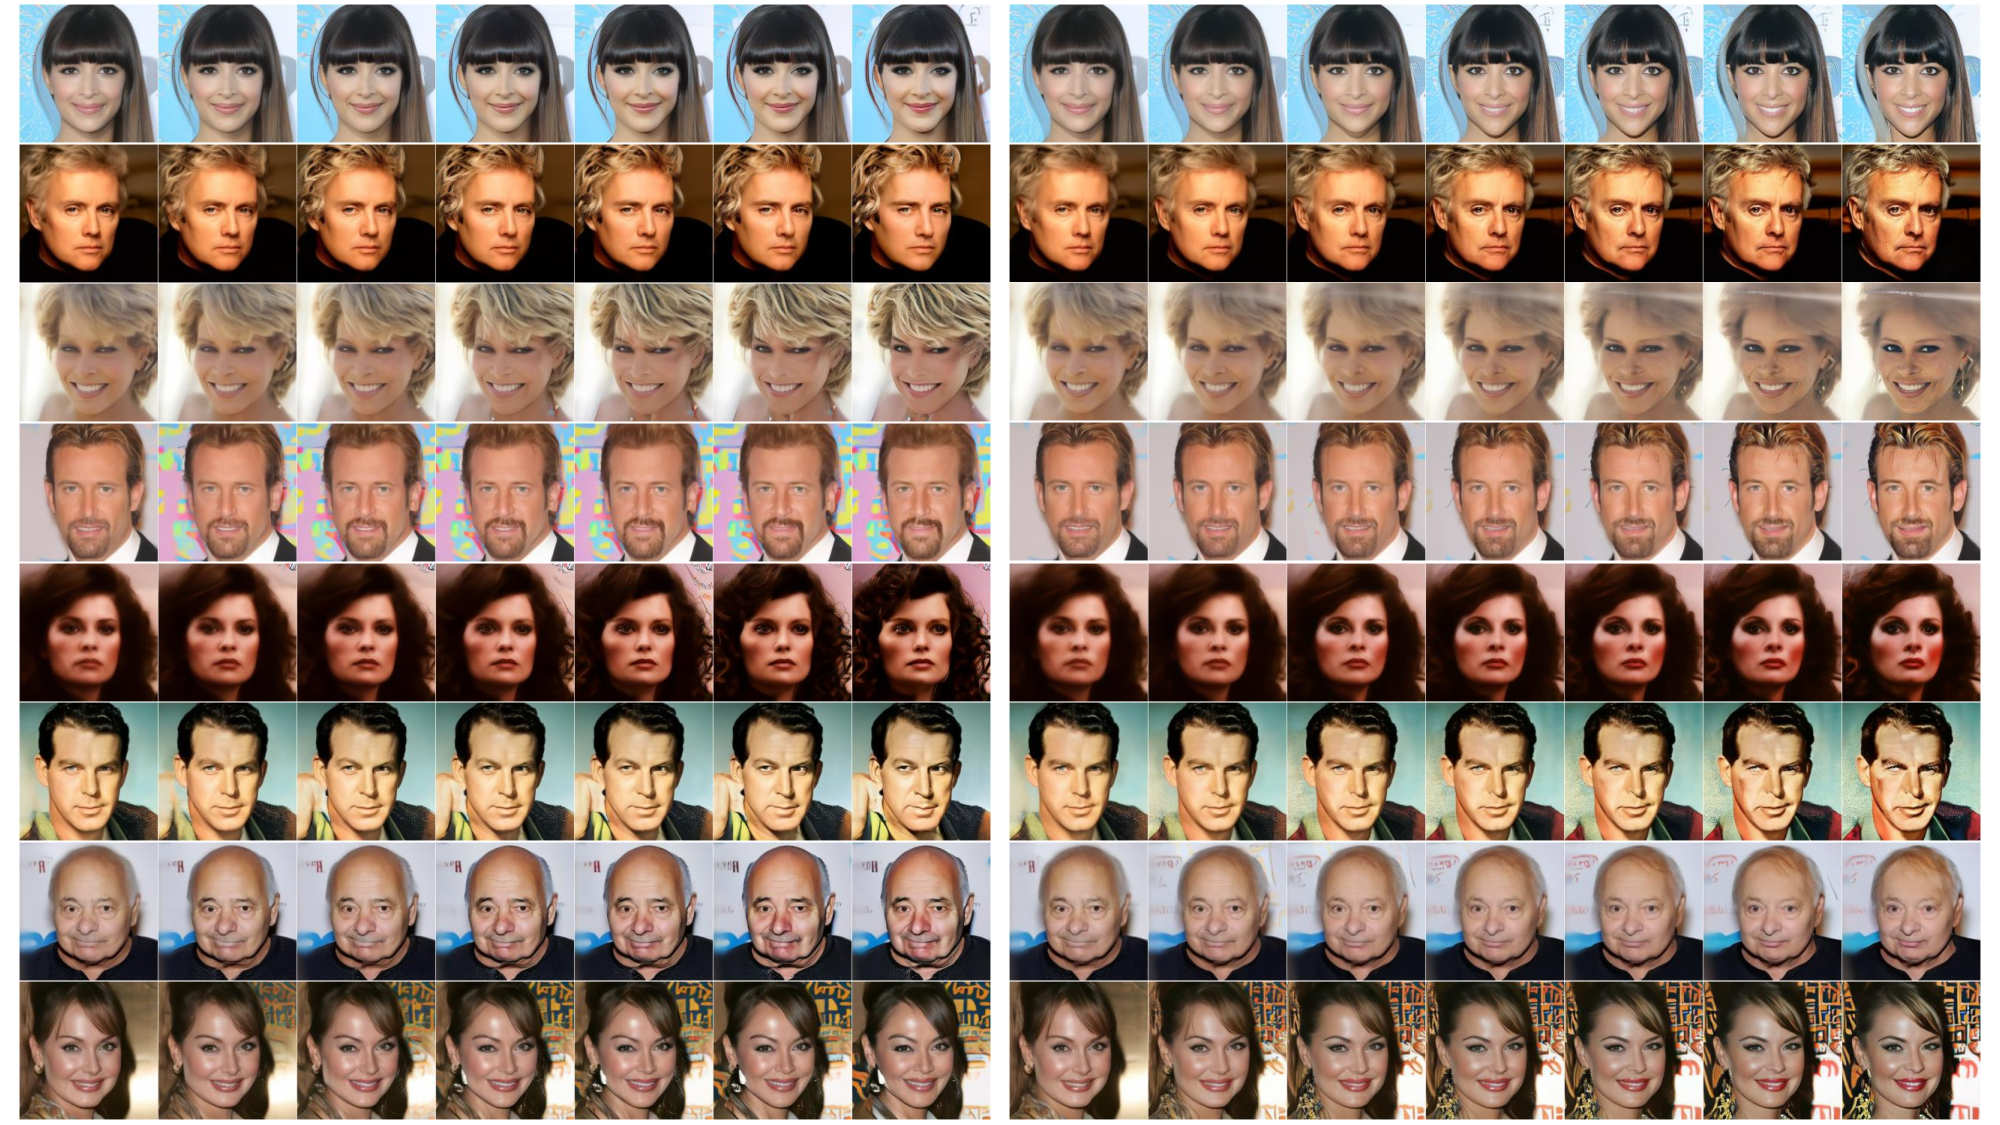
\includegraphics[width=1.0\linewidth]{figure/celeba_local_appendix_50.pdf}
%     \caption{
%     \textbf{$\boldsymbol{t=0.5T}$.} A selection of interpretable edits discovered by our feature direction in CelebA-HQ. The image on the far left represents the reconstructed original image, while the subsequent images demonstrate the interpretable edits that have been made to it.}
%     \label{fig:celeba_local_appendix_50}
% \end{figure}

% \begin{figure}[!h]
%     \centering
%     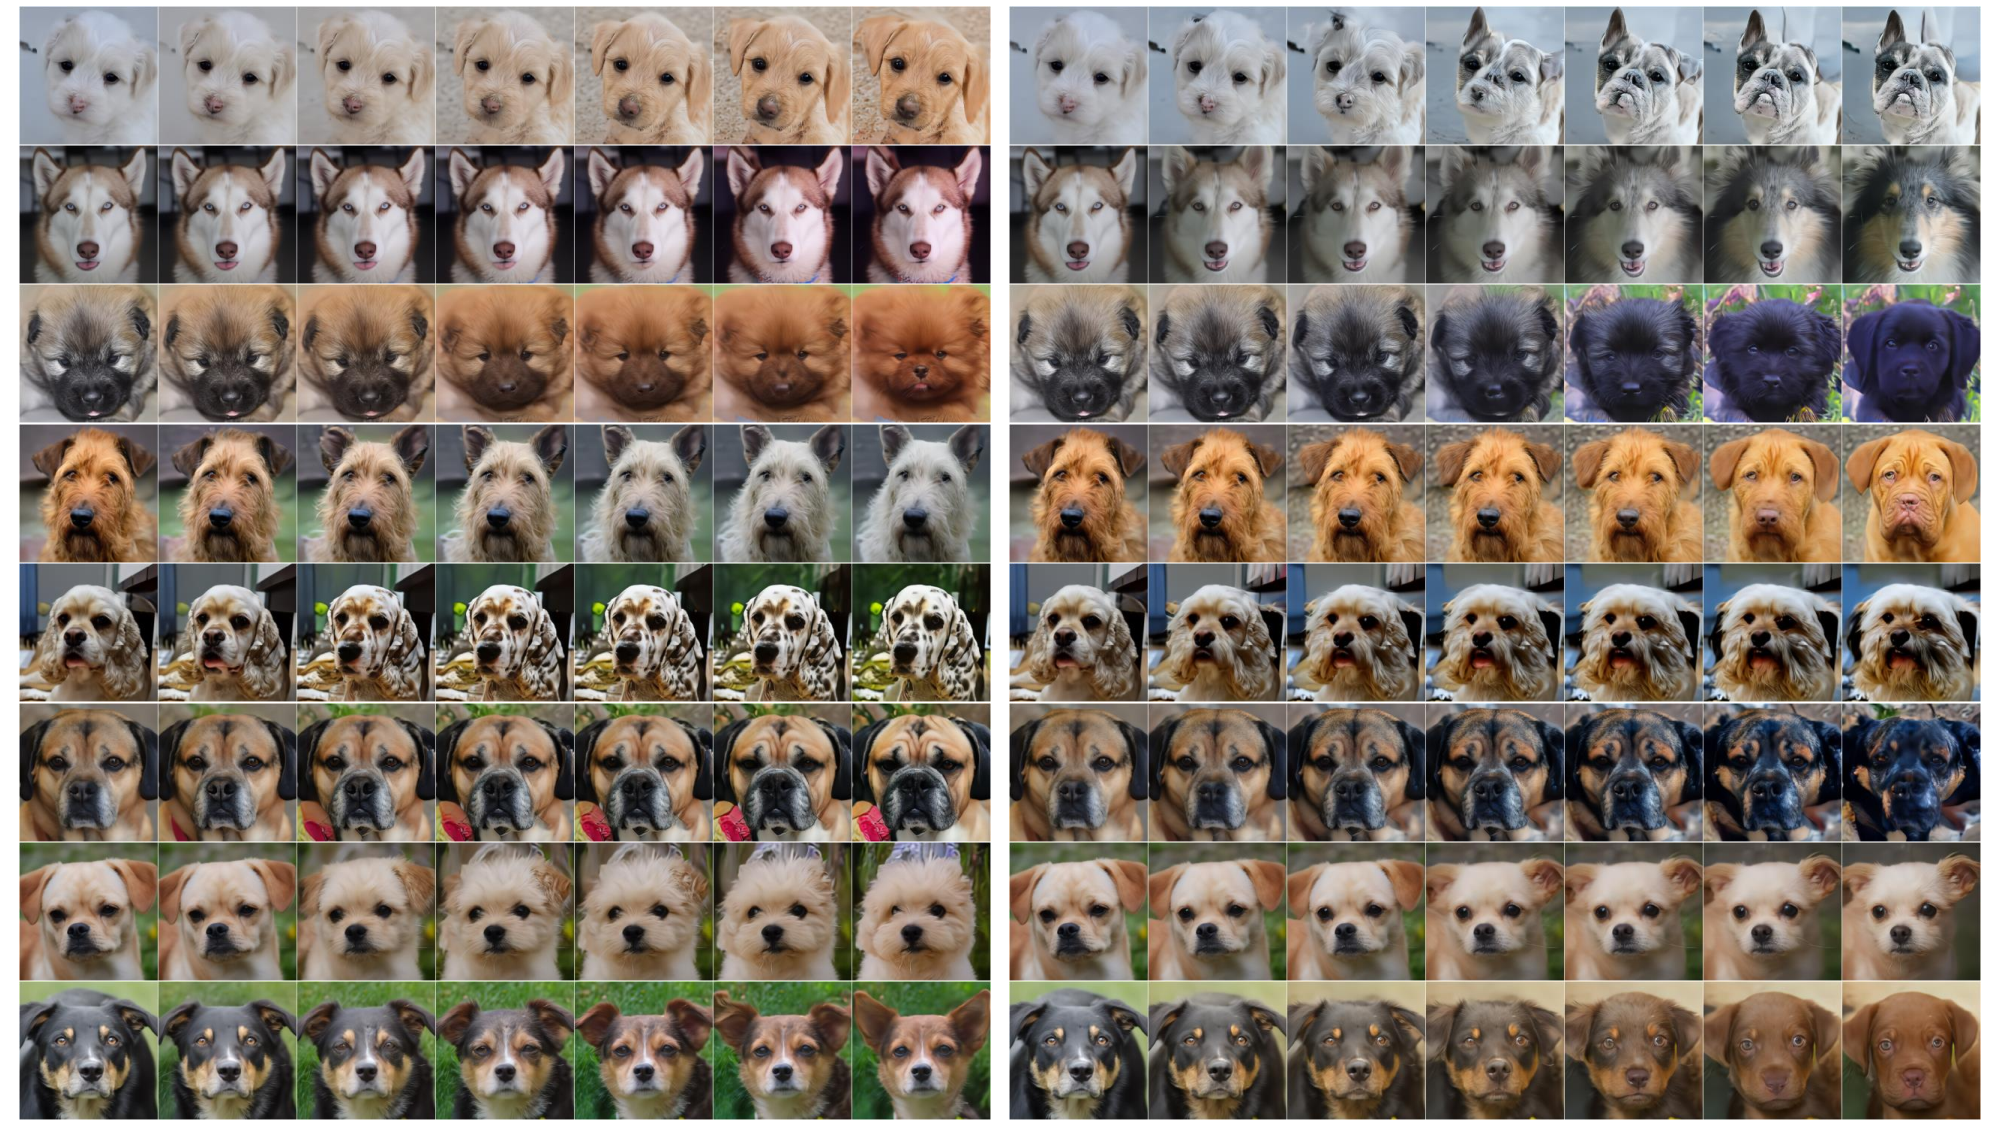
\includegraphics[width=1.0\linewidth]{figure/afhq_local_appendix.pdf}
%     \caption{
%     \textbf{$\boldsymbol{t=T}$.} A selection of interpretable edits discovered by our feature direction in AFHQ. The image on the far left represents the reconstructed original image, while the subsequent images demonstrate the interpretable edits that have been made to it.}
%     \label{fig:afhq_local_appendix}
% \end{figure}

% \begin{figure}[!h]
%     \centering
%     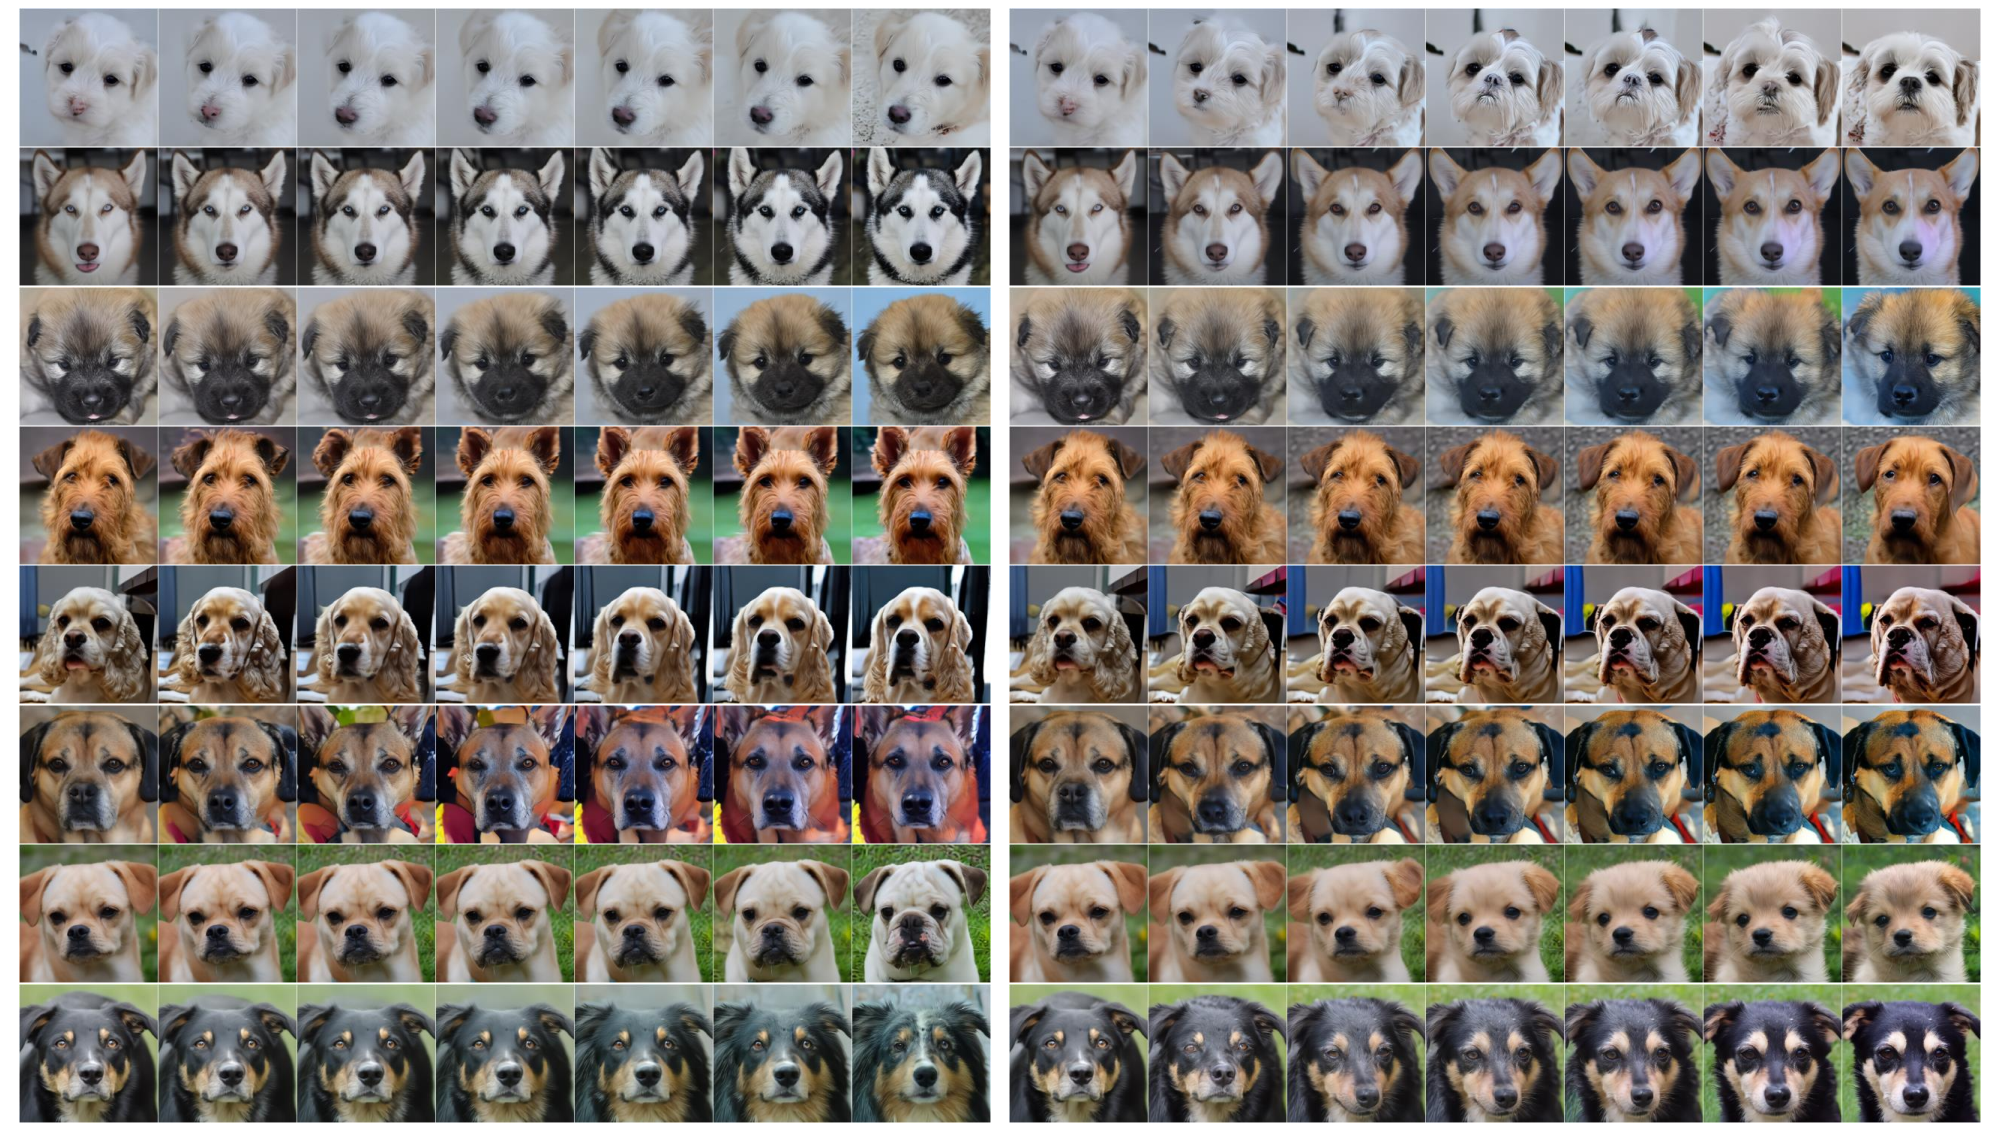
\includegraphics[width=1.0\linewidth]{figure/afhq_local_appendix_75.pdf}
%     \caption{
%     \textbf{$\boldsymbol{t=0.75T}$.} A selection of interpretable edits discovered by our feature direction in AFHQ. The image on the far left represents the reconstructed original image, while the subsequent images demonstrate the interpretable edits that have been made to it.}
%     \label{fig:afhq_local_appendix_75}
% \end{figure}

% \begin{figure}[!h]
%     \centering
%     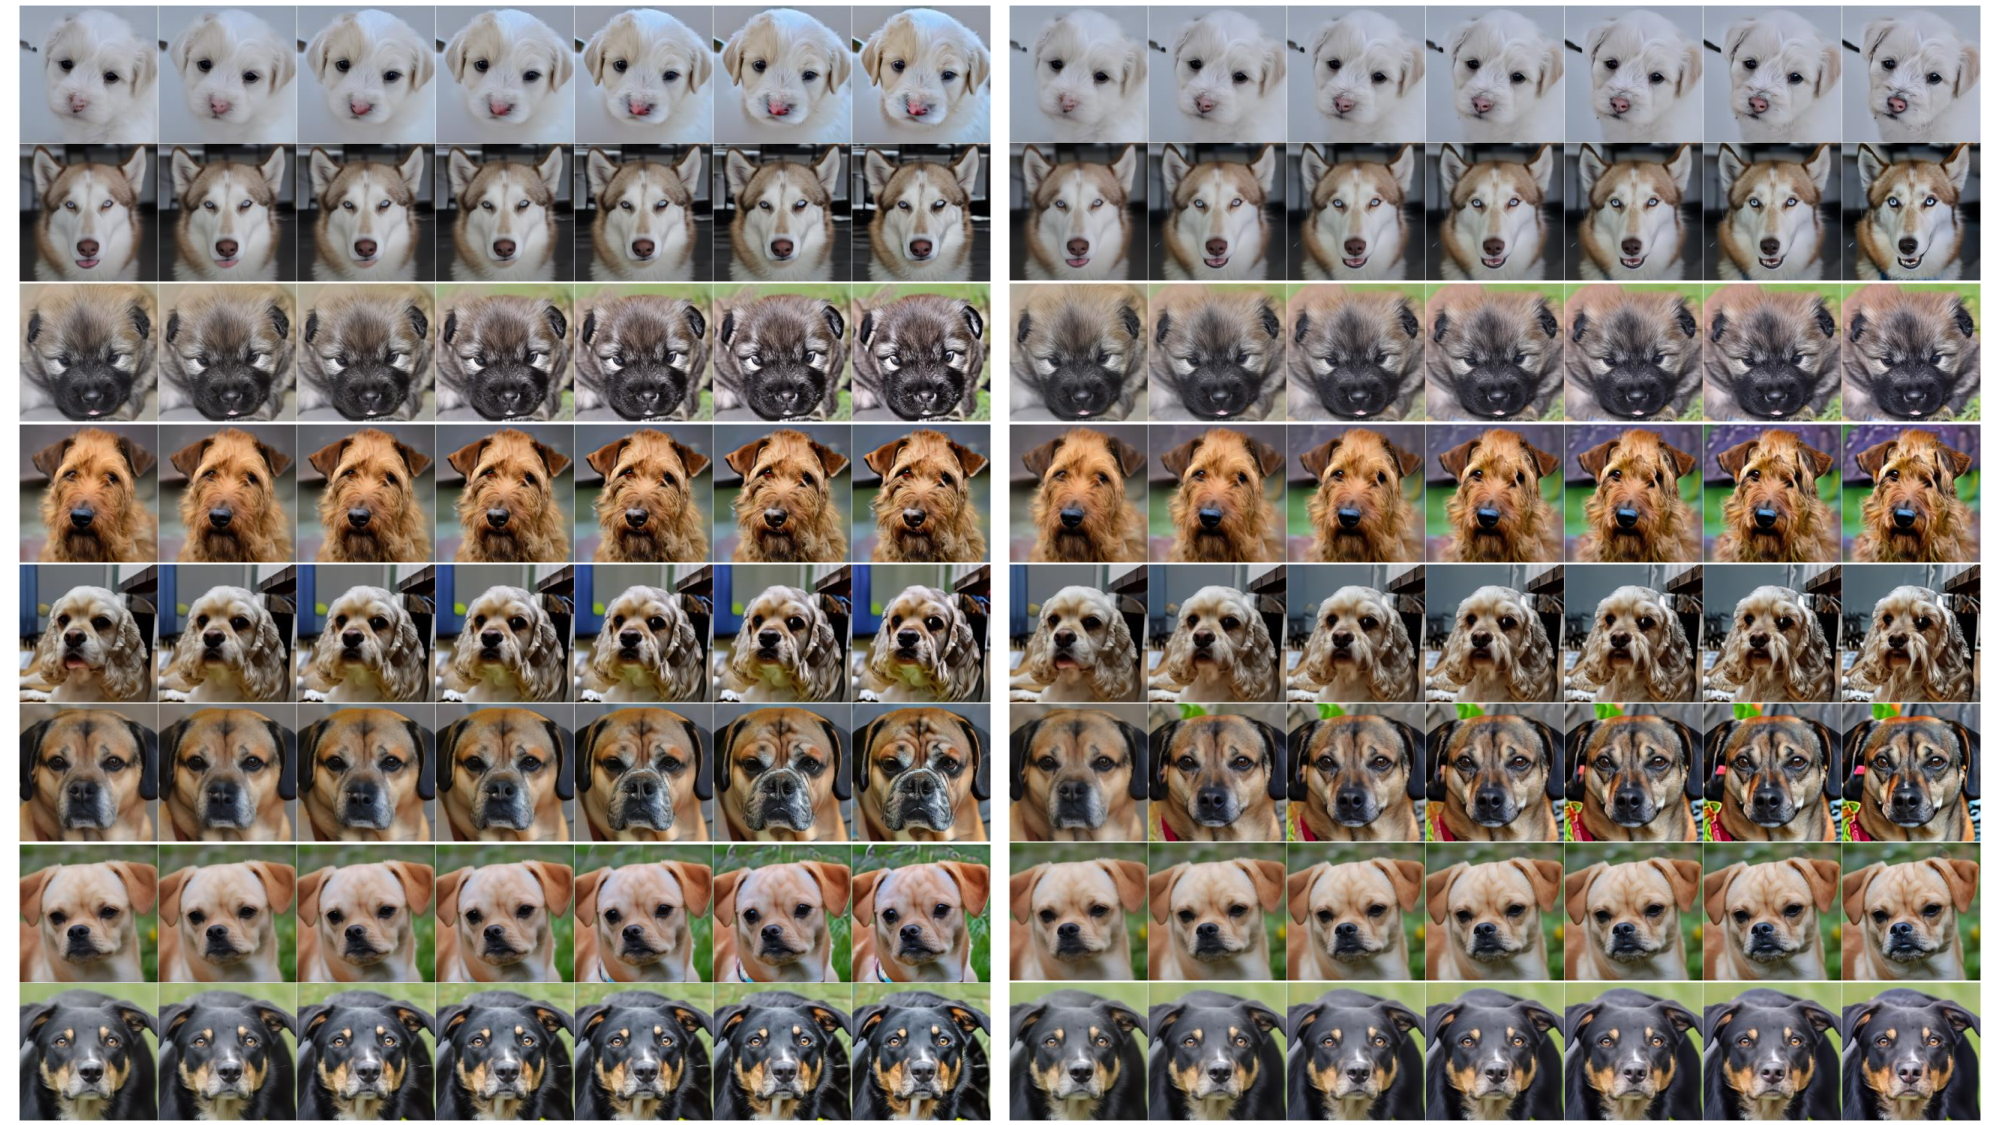
\includegraphics[width=1.0\linewidth]{figure/afhq_local_appendix_50.pdf}
%     \caption{
%     \textbf{$\boldsymbol{t=0.5T}$.} A selection of interpretable edits discovered by our feature direction in AFHQ. The image on the far left represents the reconstructed original image, while the subsequent images demonstrate the interpretable edits that have been made to it.}
%     \label{fig:afhq_local_appendix_50}
% \end{figure}

% \begin{figure}[!h]
%     \centering
%     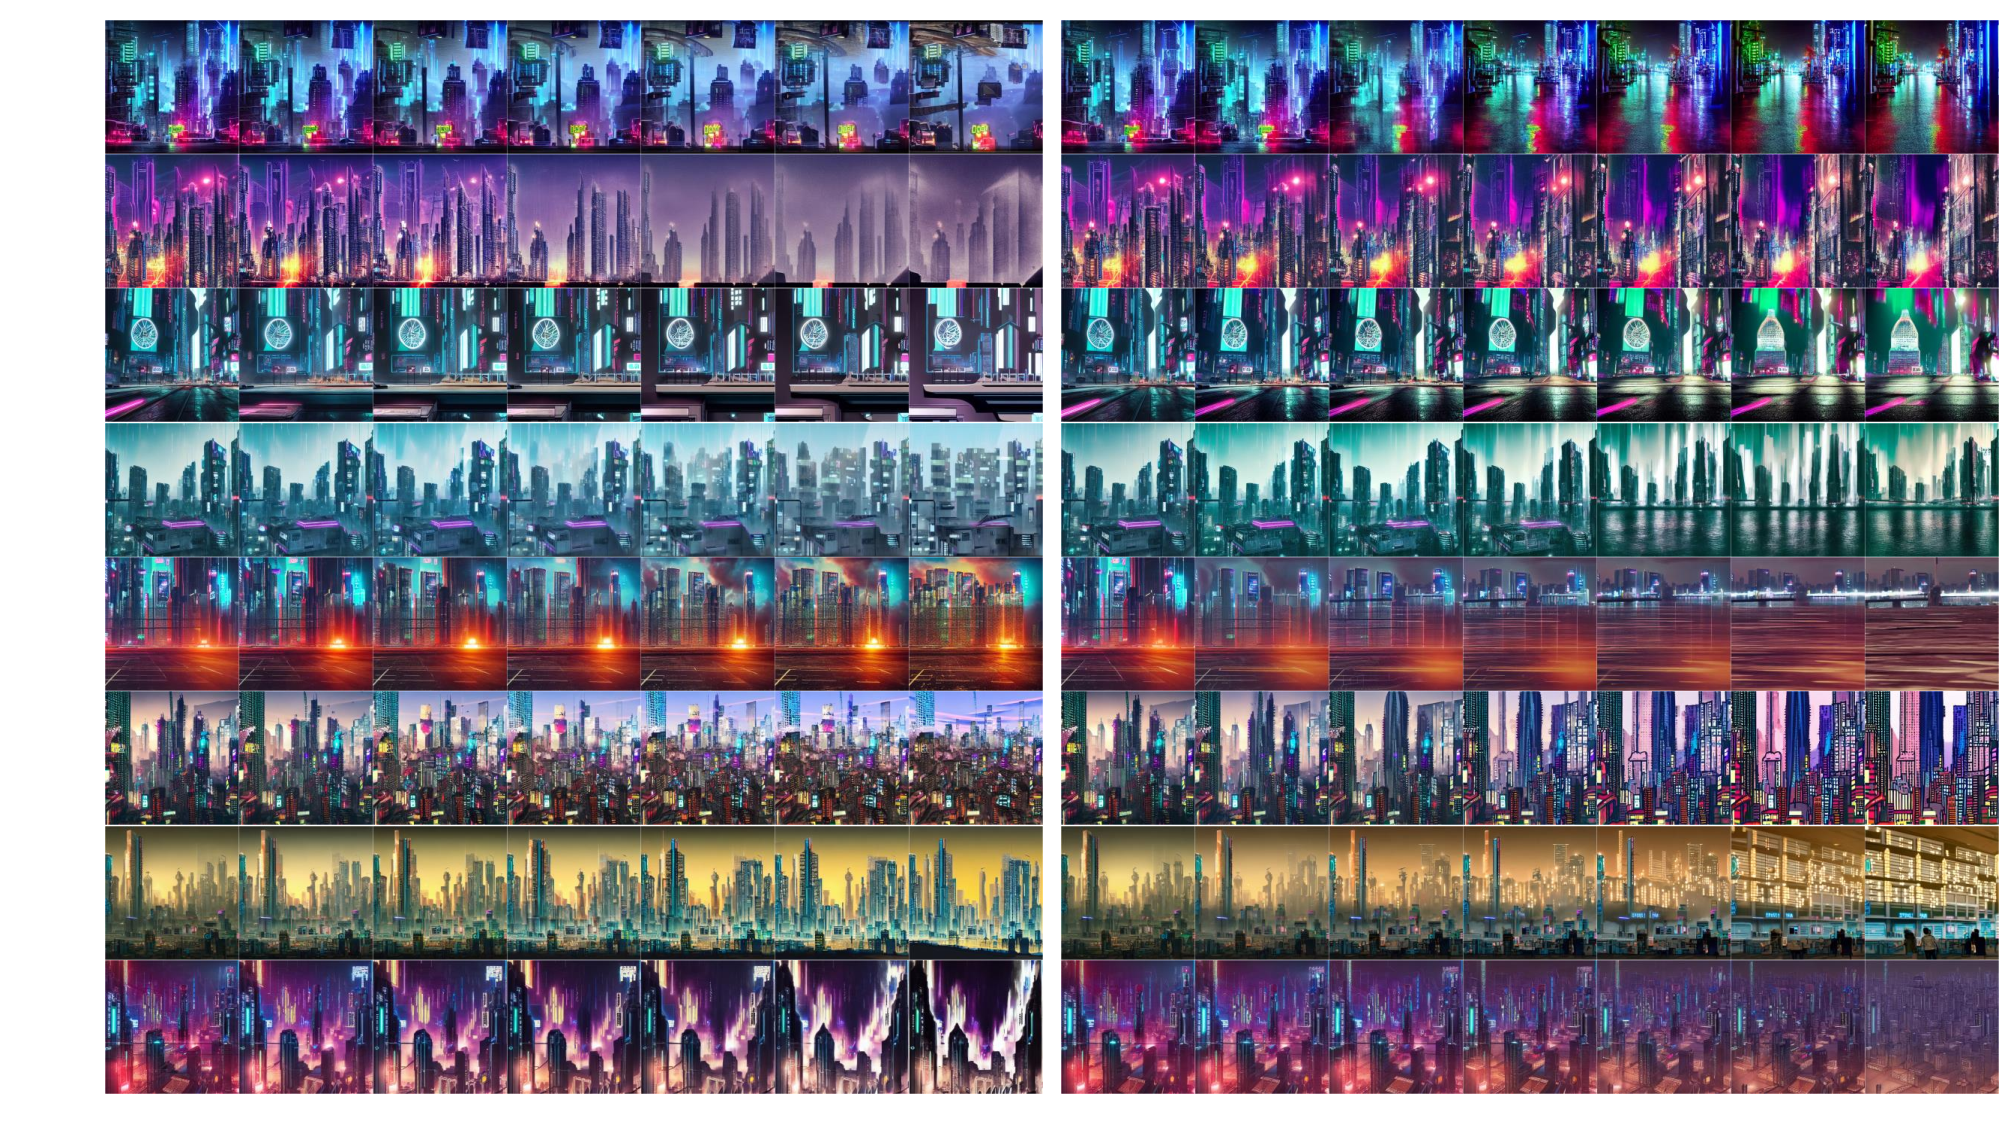
\includegraphics[width=1.0\linewidth]{figure/ldm_cyber_appendix_1T.pdf}
%     \caption{
%     \textbf{$\boldsymbol{t=T}$.} A selection of interpretable edits discovered by our feature direction in LDM with "Cyberpunk city". The image on the far left represents the reconstructed original image, while the subsequent images demonstrate the interpretable edits that have been made to it.}
%     \label{fig:ldm_cyber_appendix_1T}
% \end{figure}

% \begin{figure}[!h]
%     \centering
%     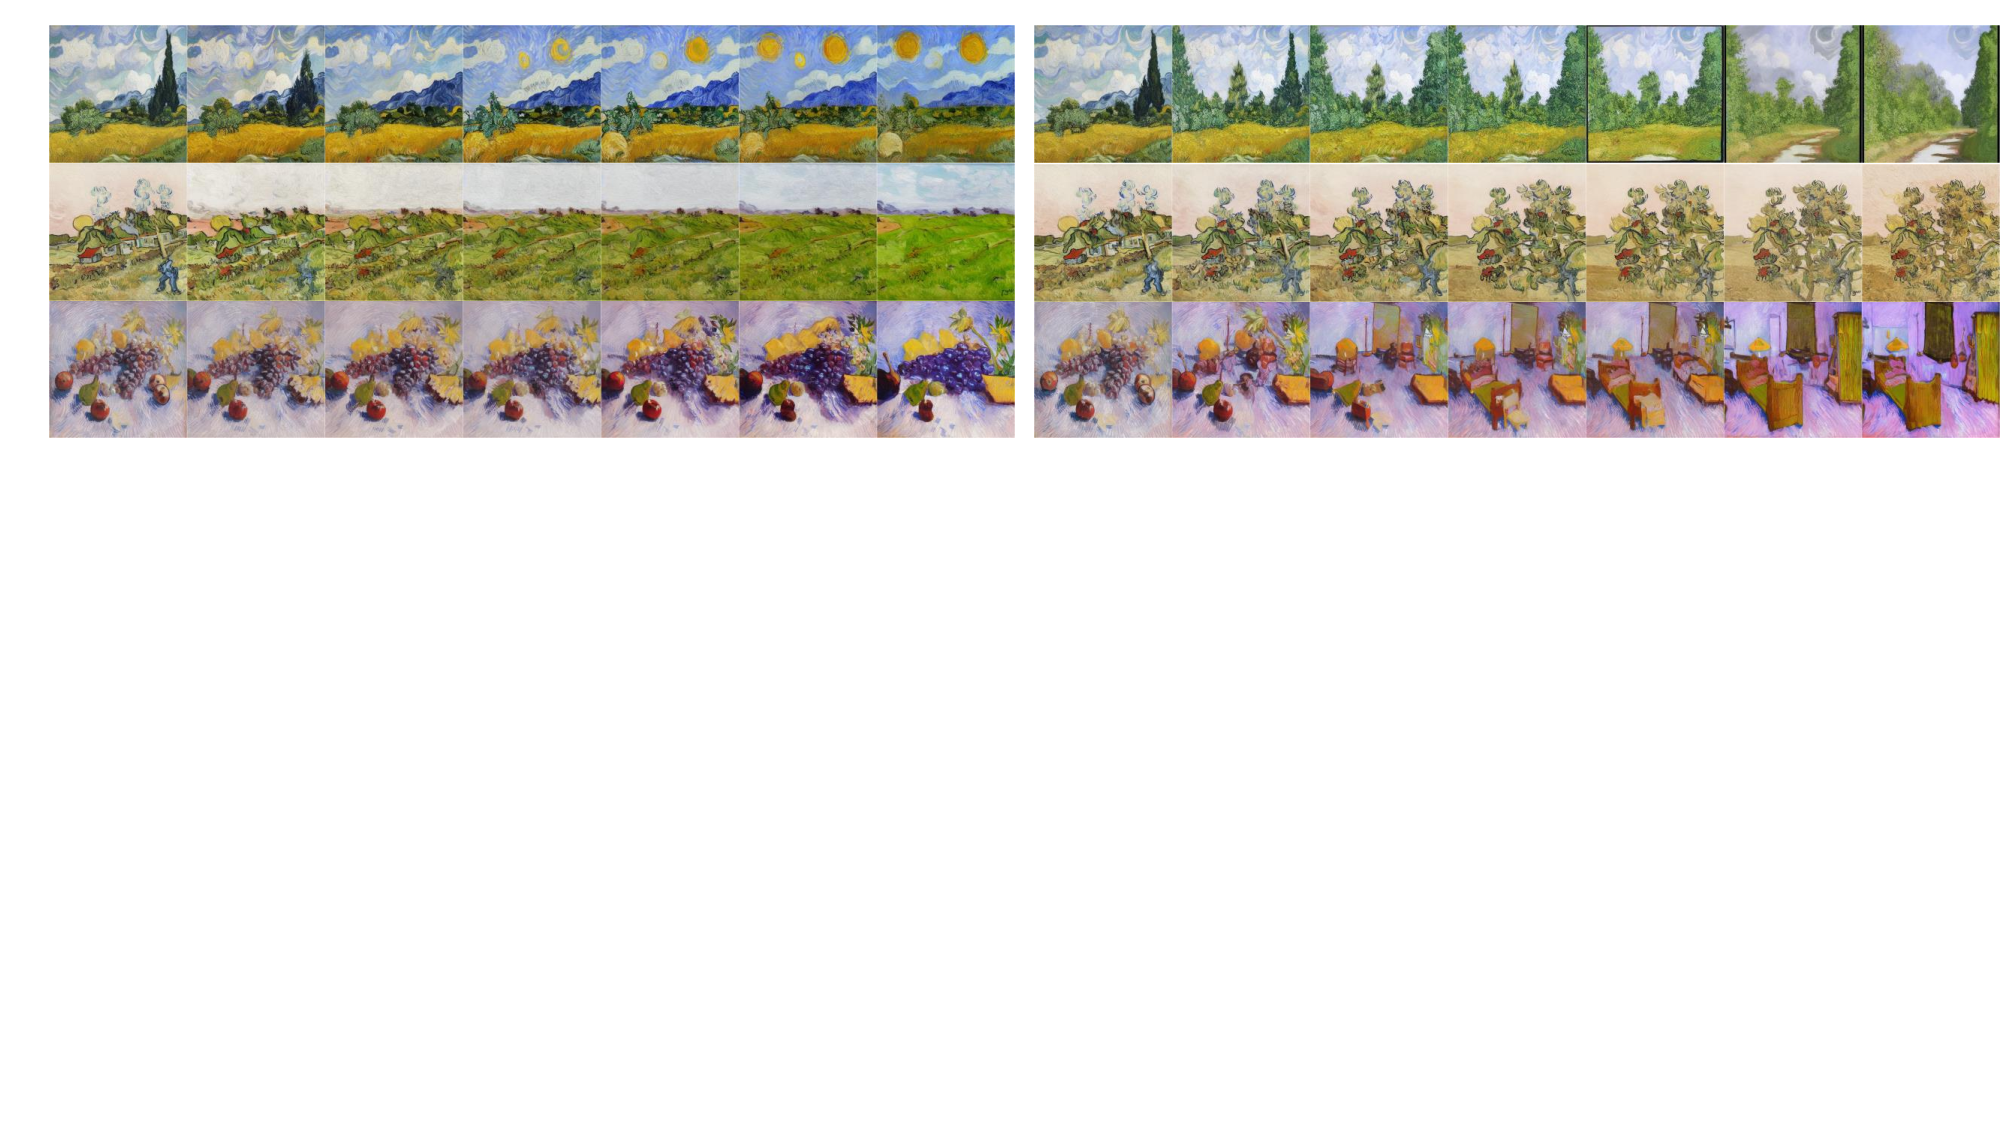
\includegraphics[width=1.0\linewidth]{figure/ldm_local_gogh_appendix_T1.pdf}
%     \caption{
%     \textbf{$\boldsymbol{t=T}$.} A selection of interpretable edits discovered by our feature direction in LDM with "Painting of VanGogh". The image on the far left represents the reconstructed original image, while the subsequent images demonstrate the interpretable edits that have been made to it.}
%     \label{fig:ldm_local_gogh_appendix_T1}
% \end{figure}

% \begin{figure}[!h]
%     \centering
%     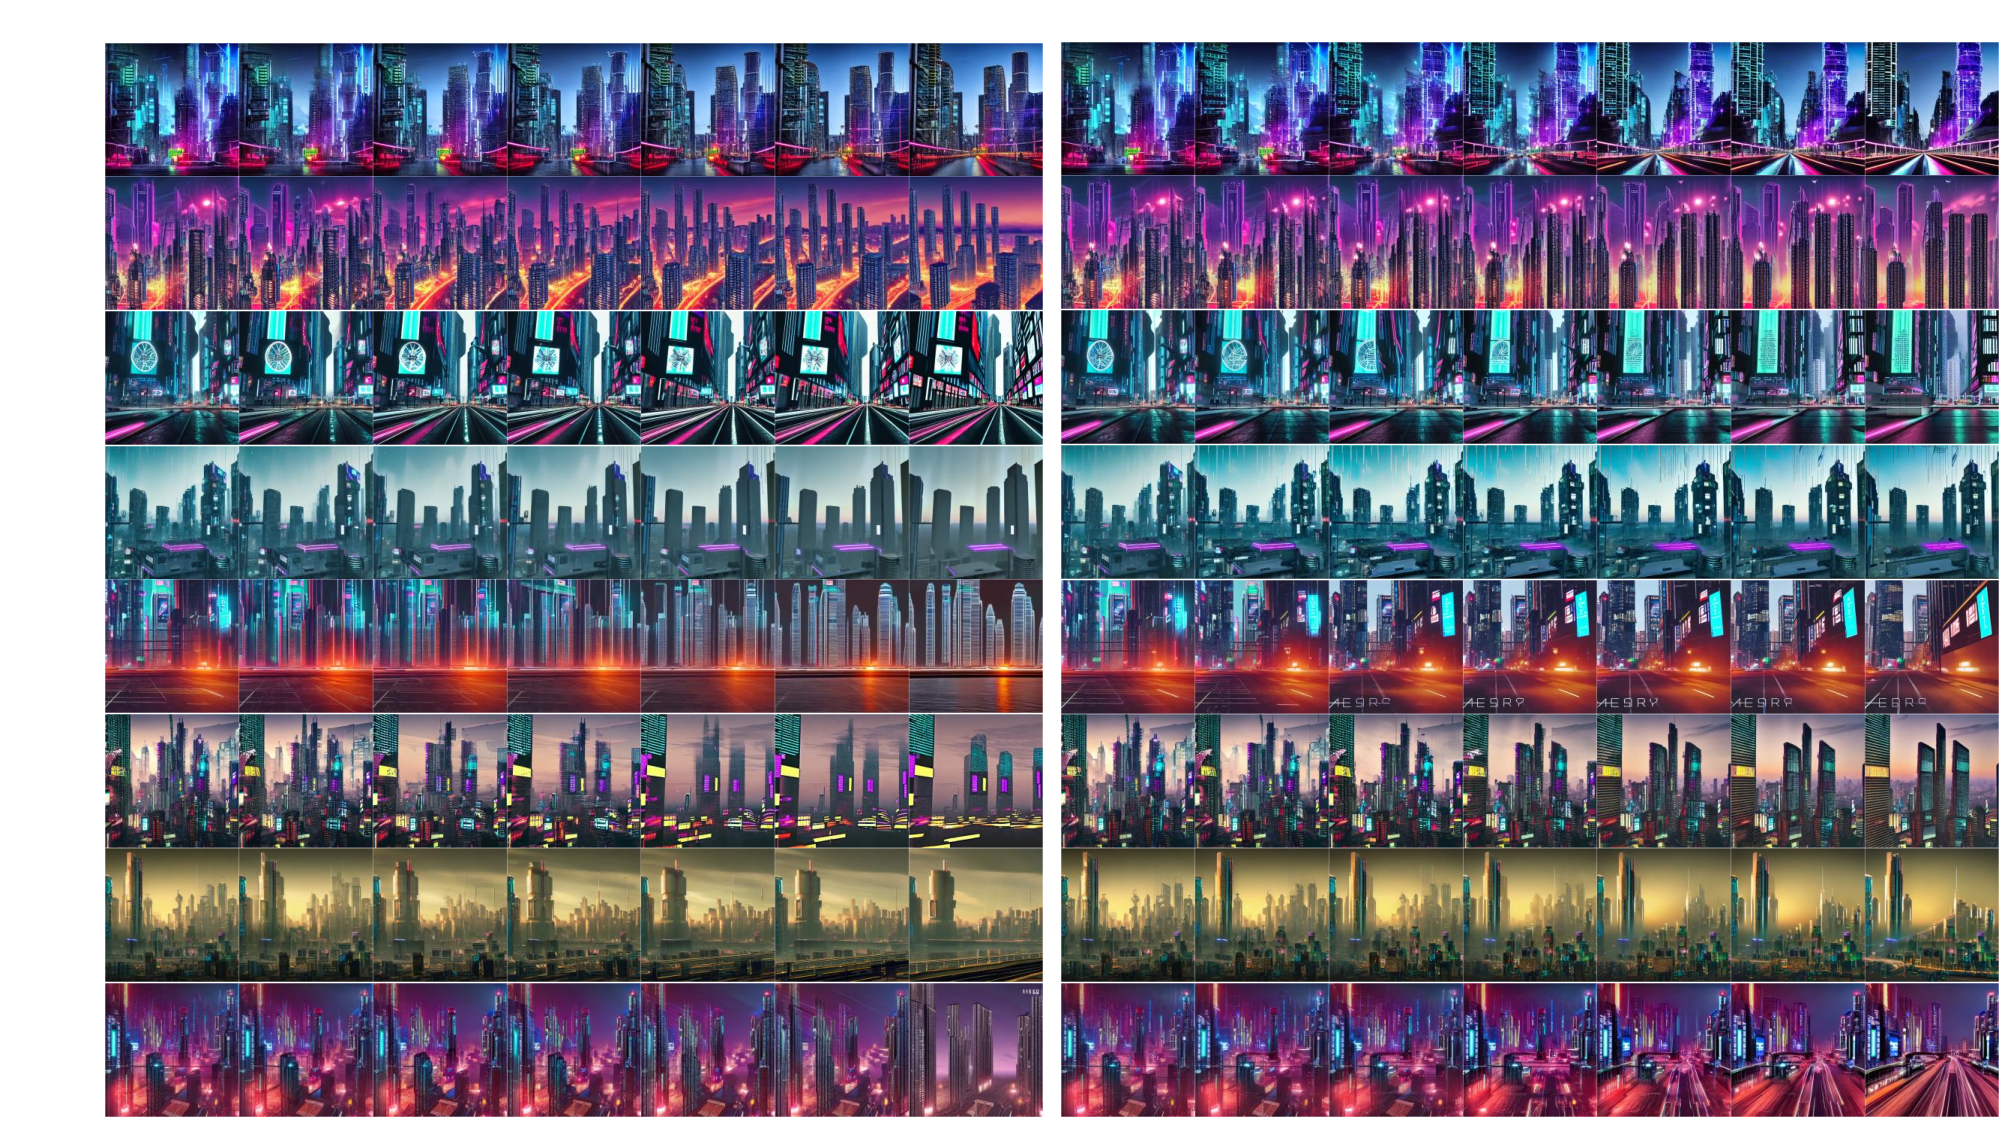
\includegraphics[width=1.0\linewidth]{figure/ldm_cyber_appendix_75T.pdf}
%     \caption{
%     \textbf{$\boldsymbol{t=0.75T}$.} A selection of interpretable edits discovered by our feature direction in LDM with "Cyberpunk city". The image on the far left represents the reconstructed original image, while the subsequent images demonstrate the interpretable edits that have been made to it.}
%     \label{fig:ldm_cyber_appendix_75T}
% \end{figure}

% \begin{figure}[!h]
%     \centering
%     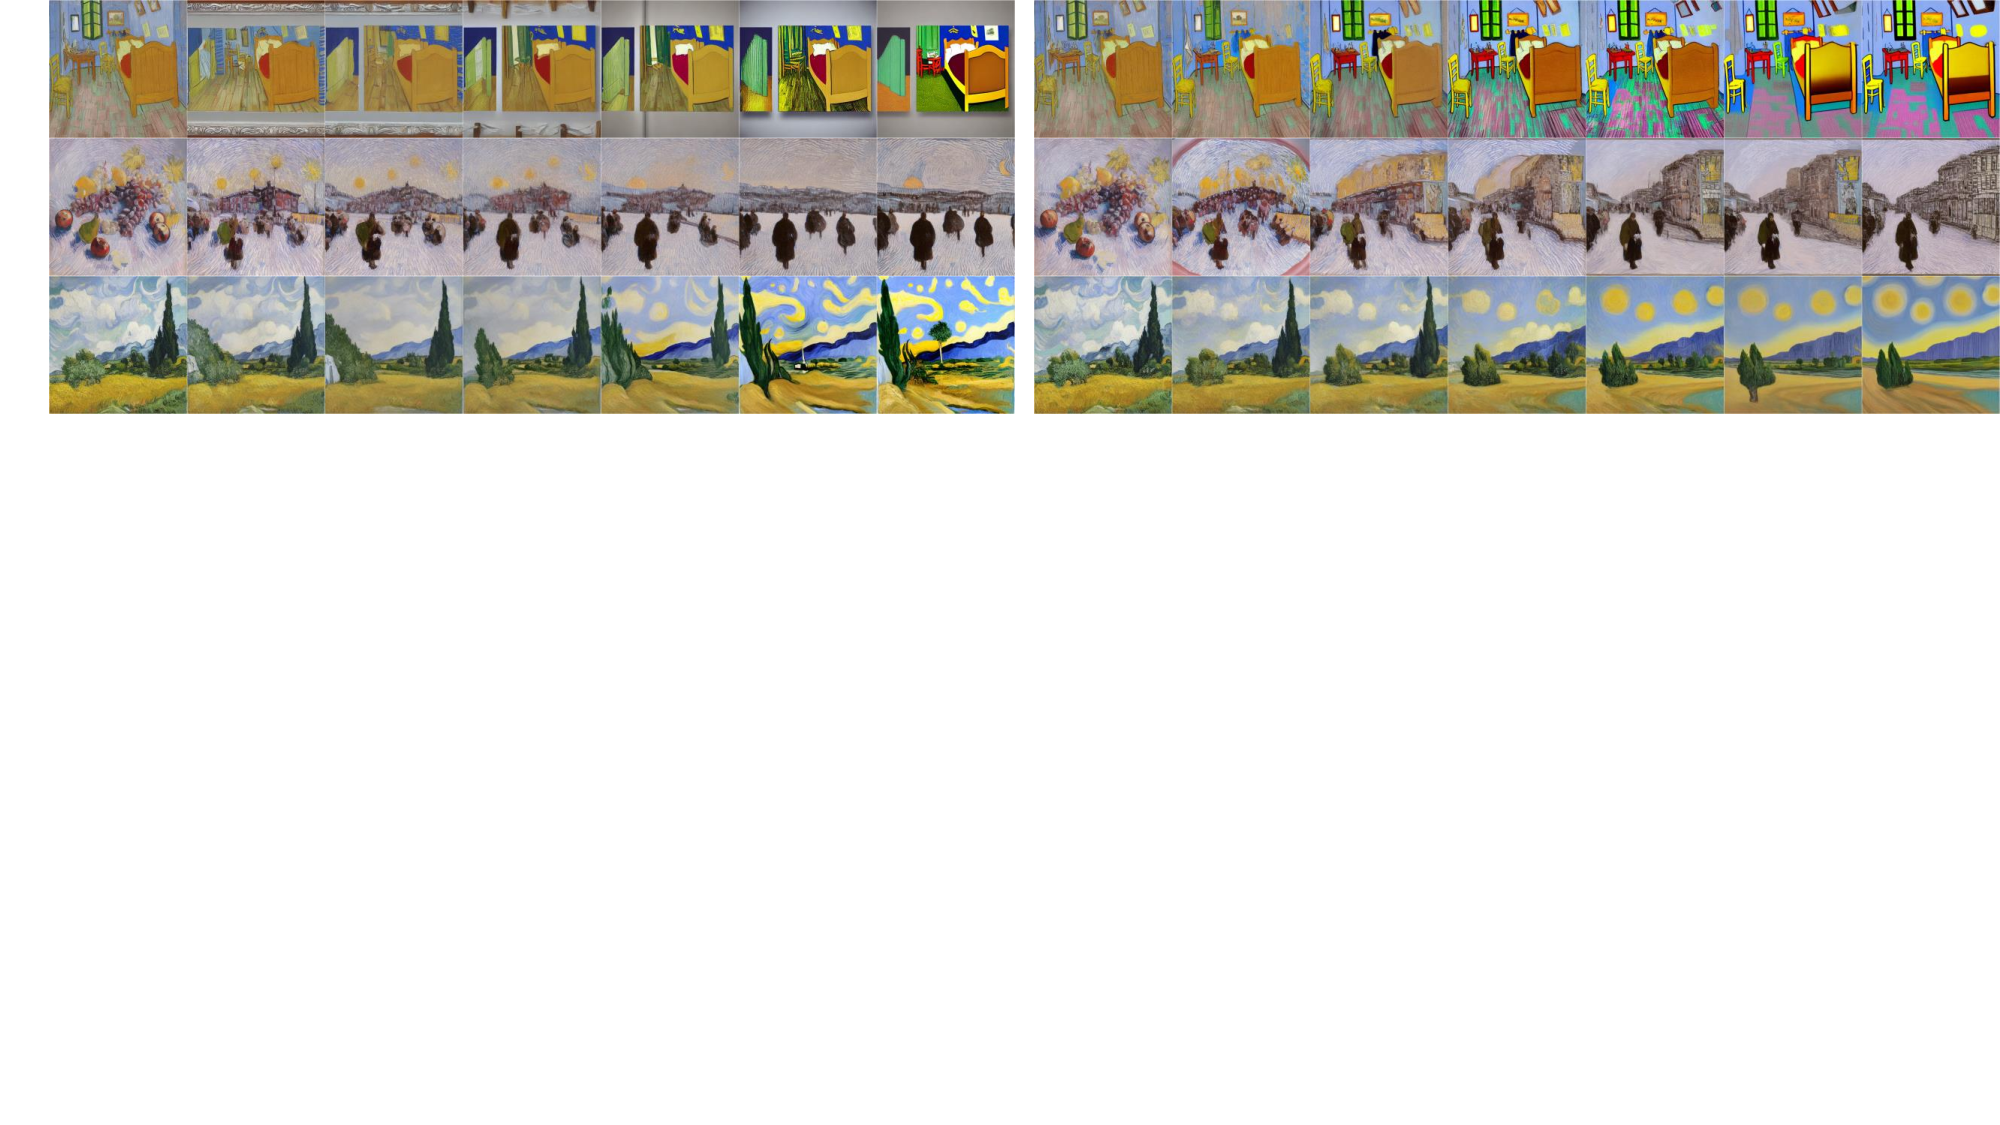
\includegraphics[width=1.0\linewidth]{figure/ldm_local_gogh_appendix_T75.pdf}
%     \caption{
%     \textbf{$\boldsymbol{t=0.75T}$.} A selection of interpretable edits discovered by our feature direction in LDM with "Painting of VanGogh". The image on the far left represents the reconstructed original image, while the subsequent images demonstrate the interpretable edits that have been made to it.}
%     \label{fig:ldm_local_gogh_appendix_T75}
% \end{figure}

% \begin{figure}[!h]
%     \centering
%     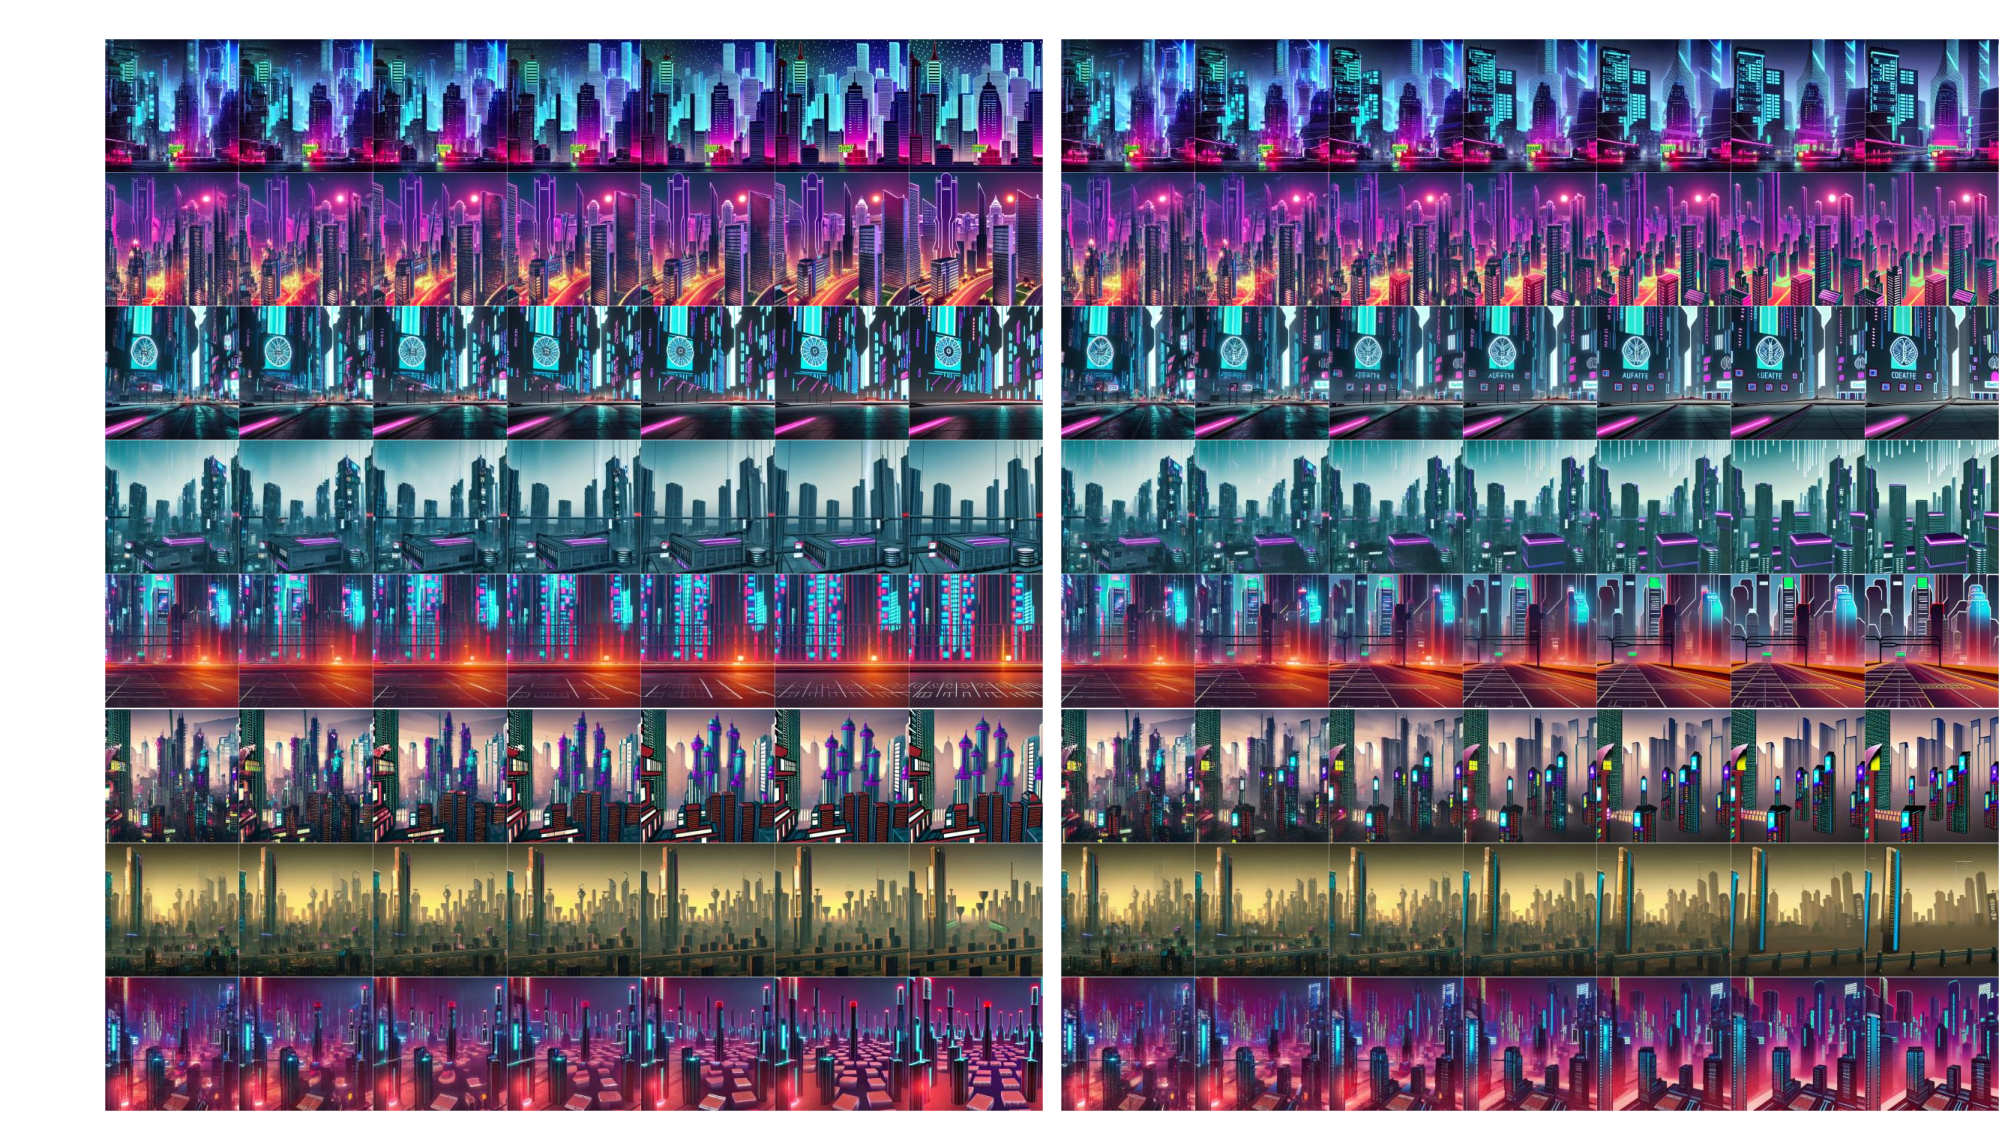
\includegraphics[width=1.0\linewidth]{figure/ldm_cyber_appendix_5T.pdf}
%     \caption{
%     \textbf{$\boldsymbol{t=0.5T}$.} A selection of interpretable edits discovered by our feature direction in LDM with "Cyberpunk city". The image on the far left represents the reconstructed original image, while the subsequent images demonstrate the interpretable edits that have been made to it.}
%     \label{fig:ldm_cyber_appendix_5T}
% \end{figure}

% \begin{figure}[!h]
%     \centering
%     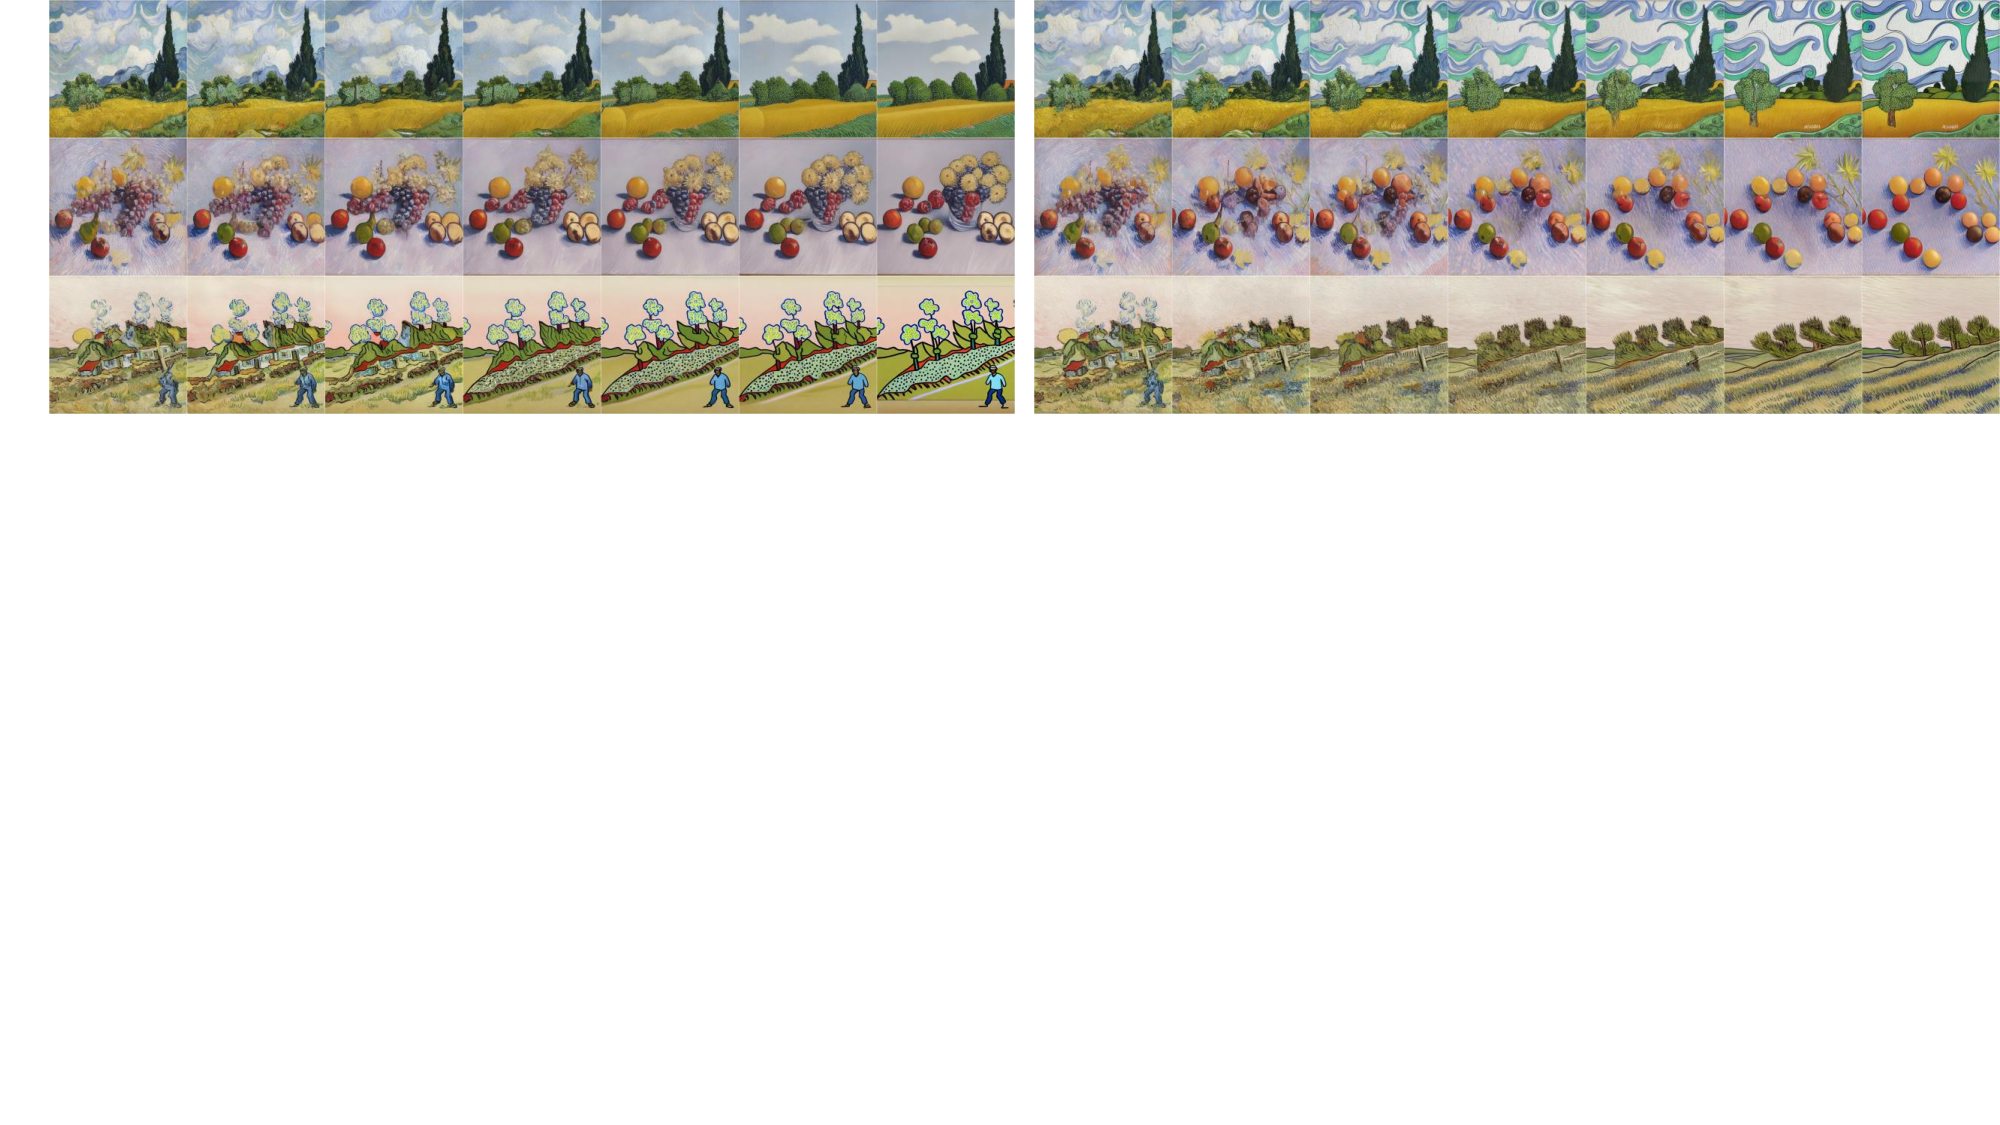
\includegraphics[width=1.0\linewidth]{figure/ldm_local_gogh_appendix_T5.pdf}
%     \caption{
%     \textbf{$\boldsymbol{t=0.5T}$.} A selection of interpretable edits discovered by our feature direction in LDM with "Painting of VanGogh". The image on the far left represents the reconstructed original image, while the subsequent images demonstrate the interpretable edits that have been made to it.}
%     \label{fig:ldm_local_gogh_appendix_T5}
% \end{figure}


% \clearpage
% \subsection{Global feature direction}
% \label{appendix:global}

% \begin{figure}[!h]
%     \centering
%     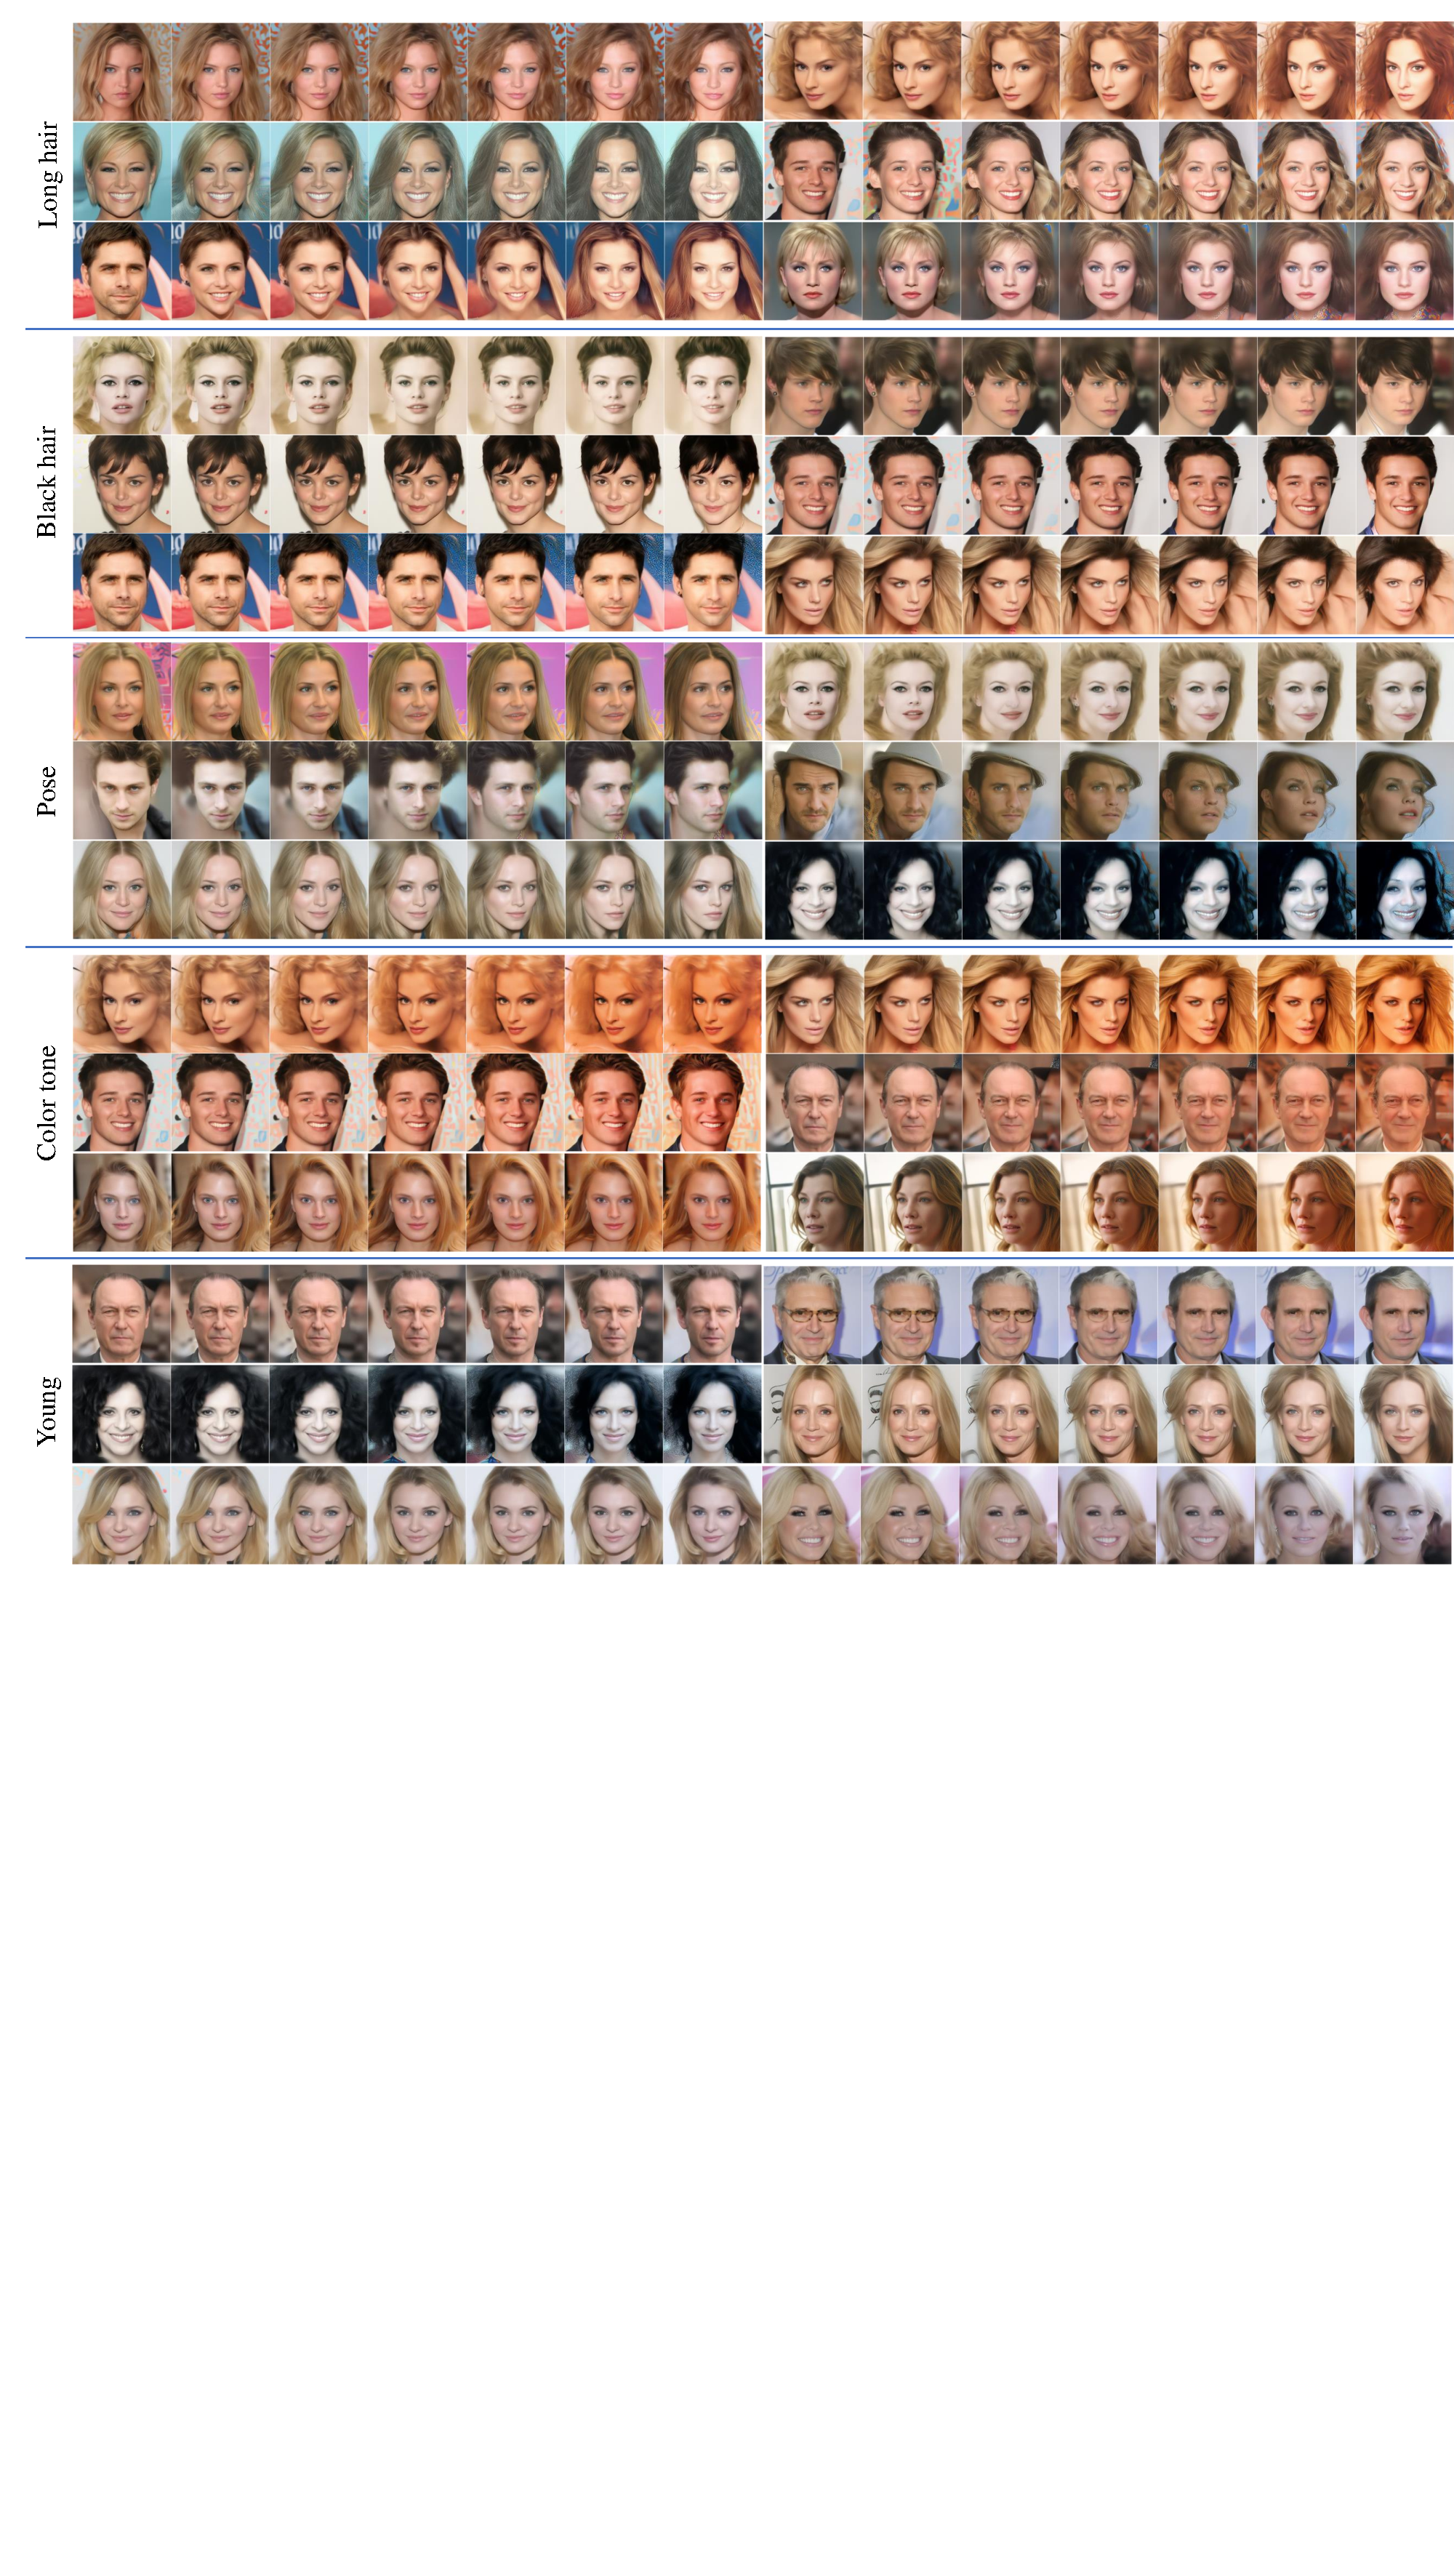
\includegraphics[width=1.0\linewidth]{figure/celeba_global_appendix.pdf}
%     \caption{
%     A selection of interpretable edits discovered by our global feature direction in CelebA-HQ. The image on the far left represents the reconstructed original image, while the subsequent images demonstrate the interpretable edits that have been made to it.}
%     \label{fig:celeba_global_appendix}
% \end{figure}

% \begin{figure}[!t]
%     \centering
%     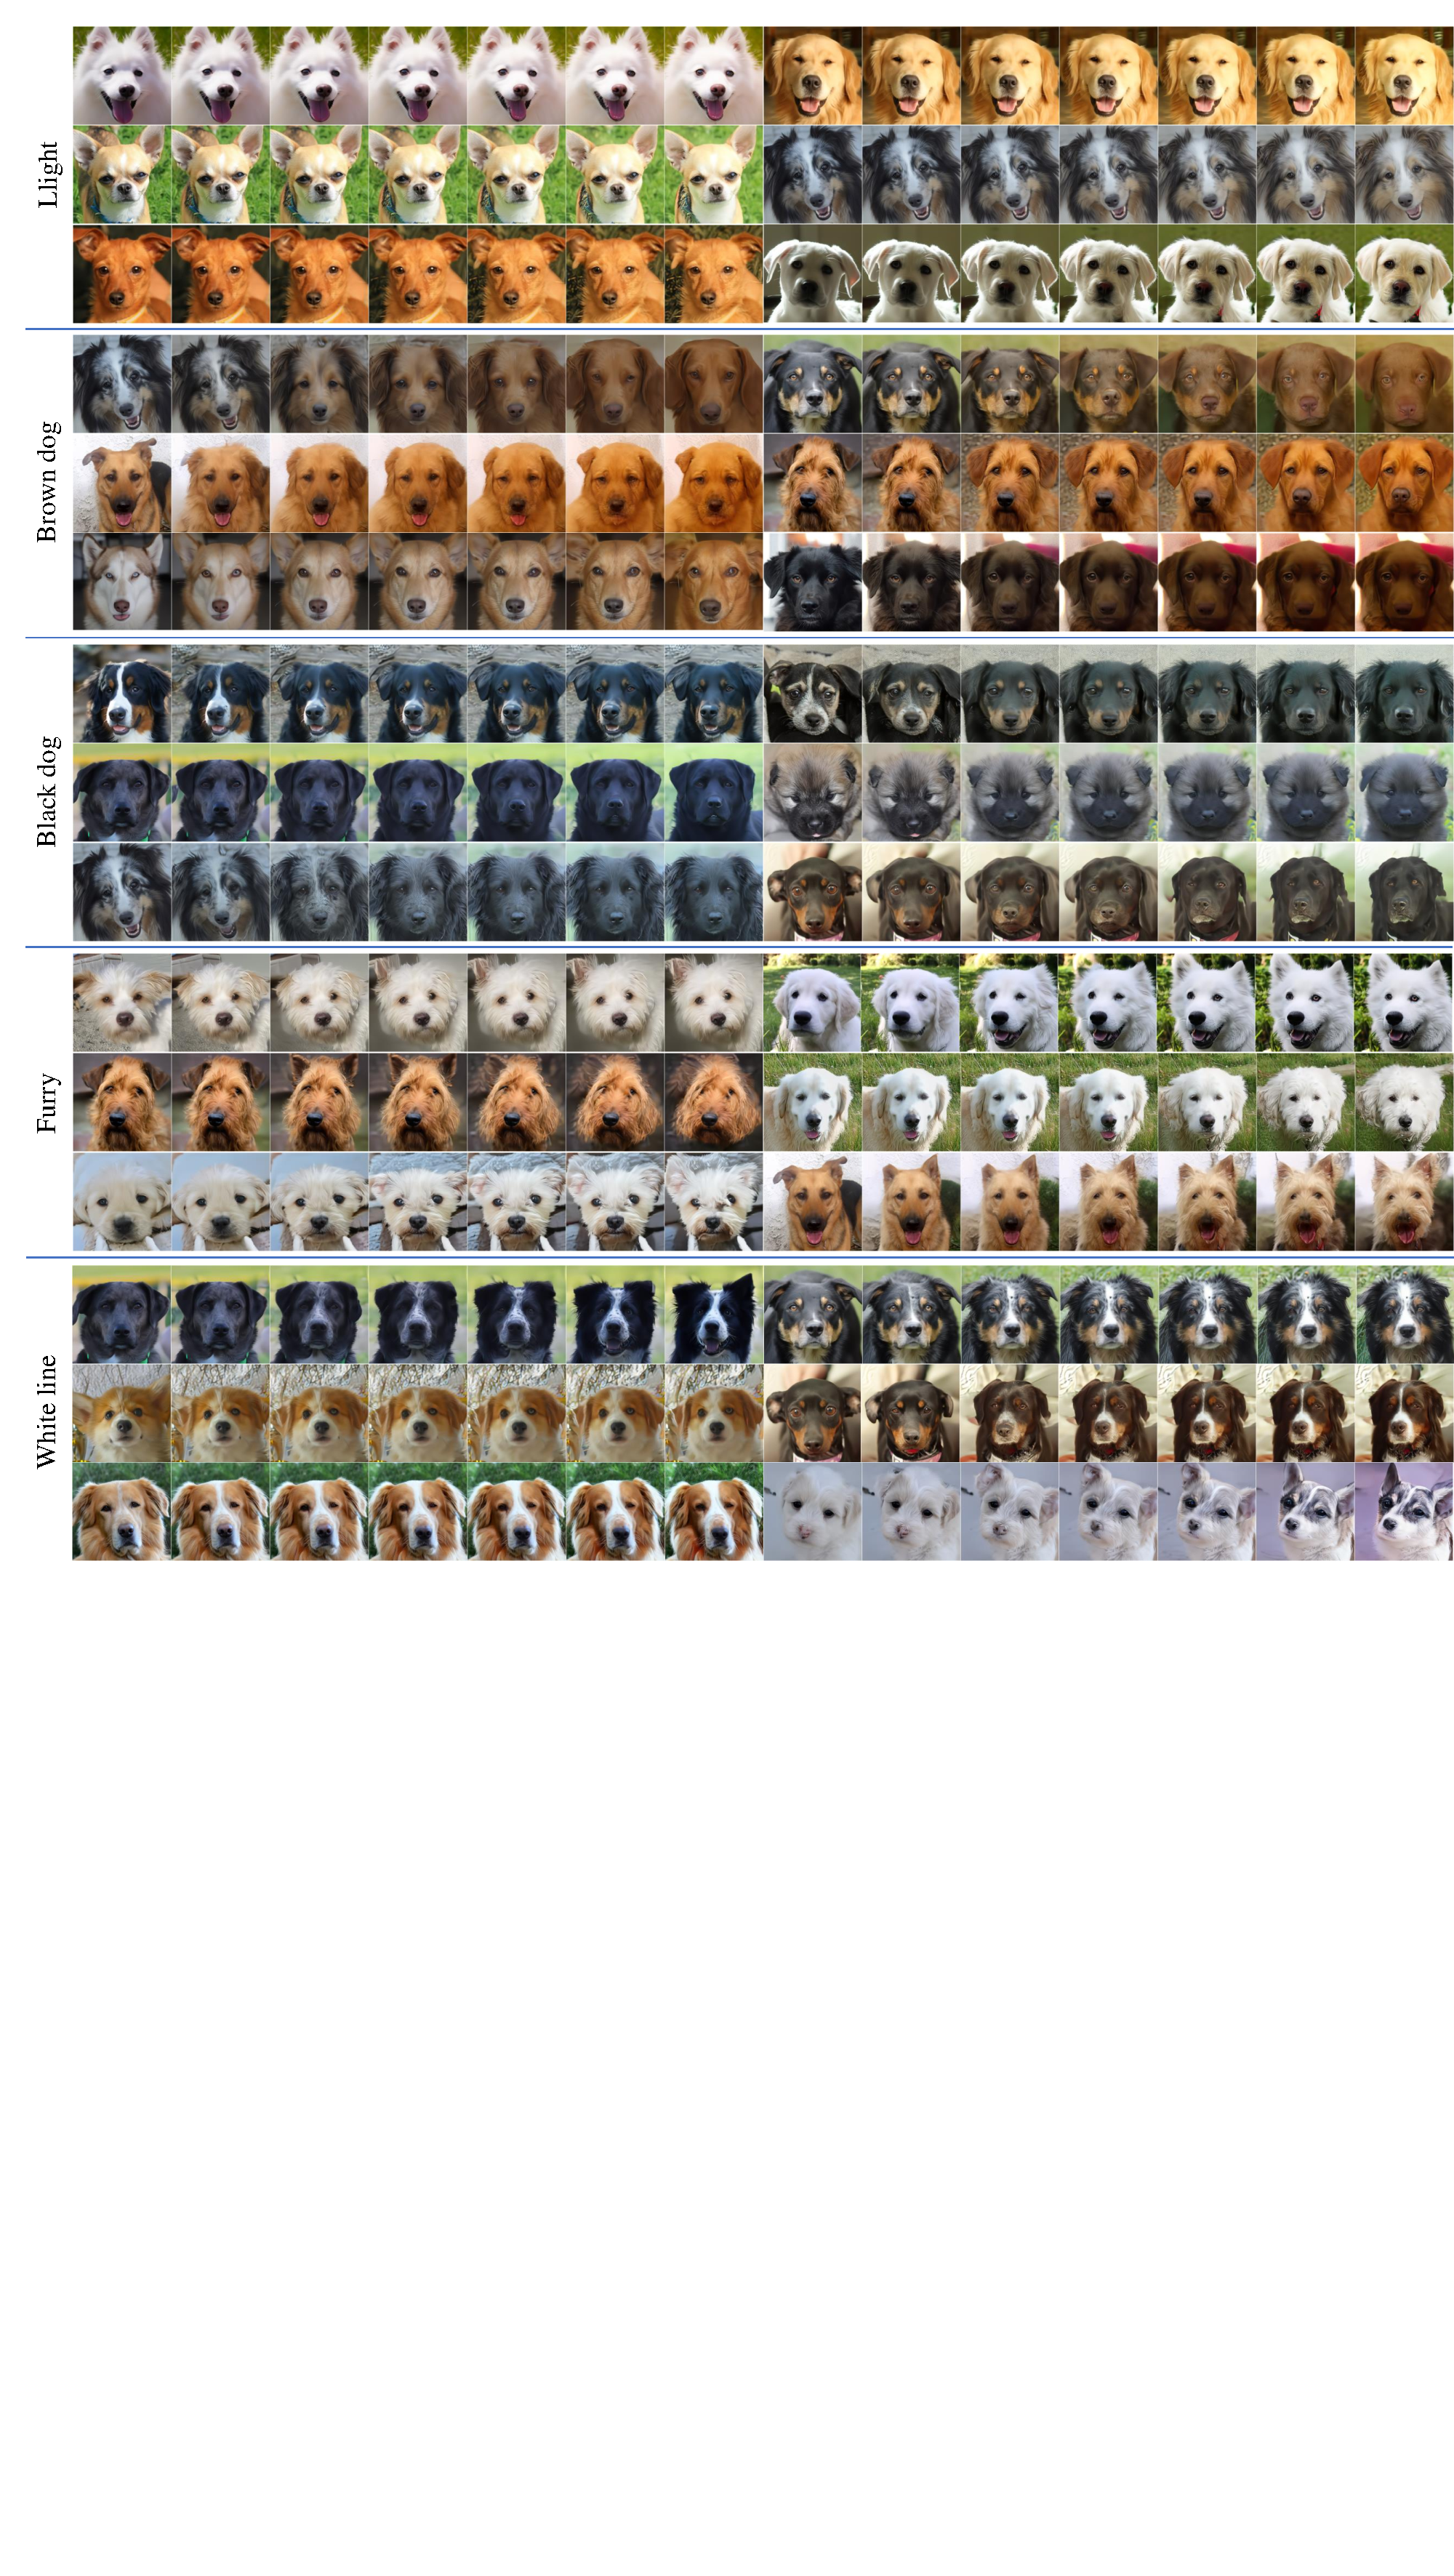
\includegraphics[width=1.0\linewidth]{figure/afhq_global_appendix2.pdf}
%     \caption{
%     A selection of interpretable edits discovered by our global feature direction in AFHQ. The image on the far left represents the reconstructed original image, while the subsequent images demonstrate the interpretable edits that have been made to it.}
%     \label{fig:afhq_global_appendix2}
% \end{figure}

% \begin{figure}[!t]
%     \centering
%     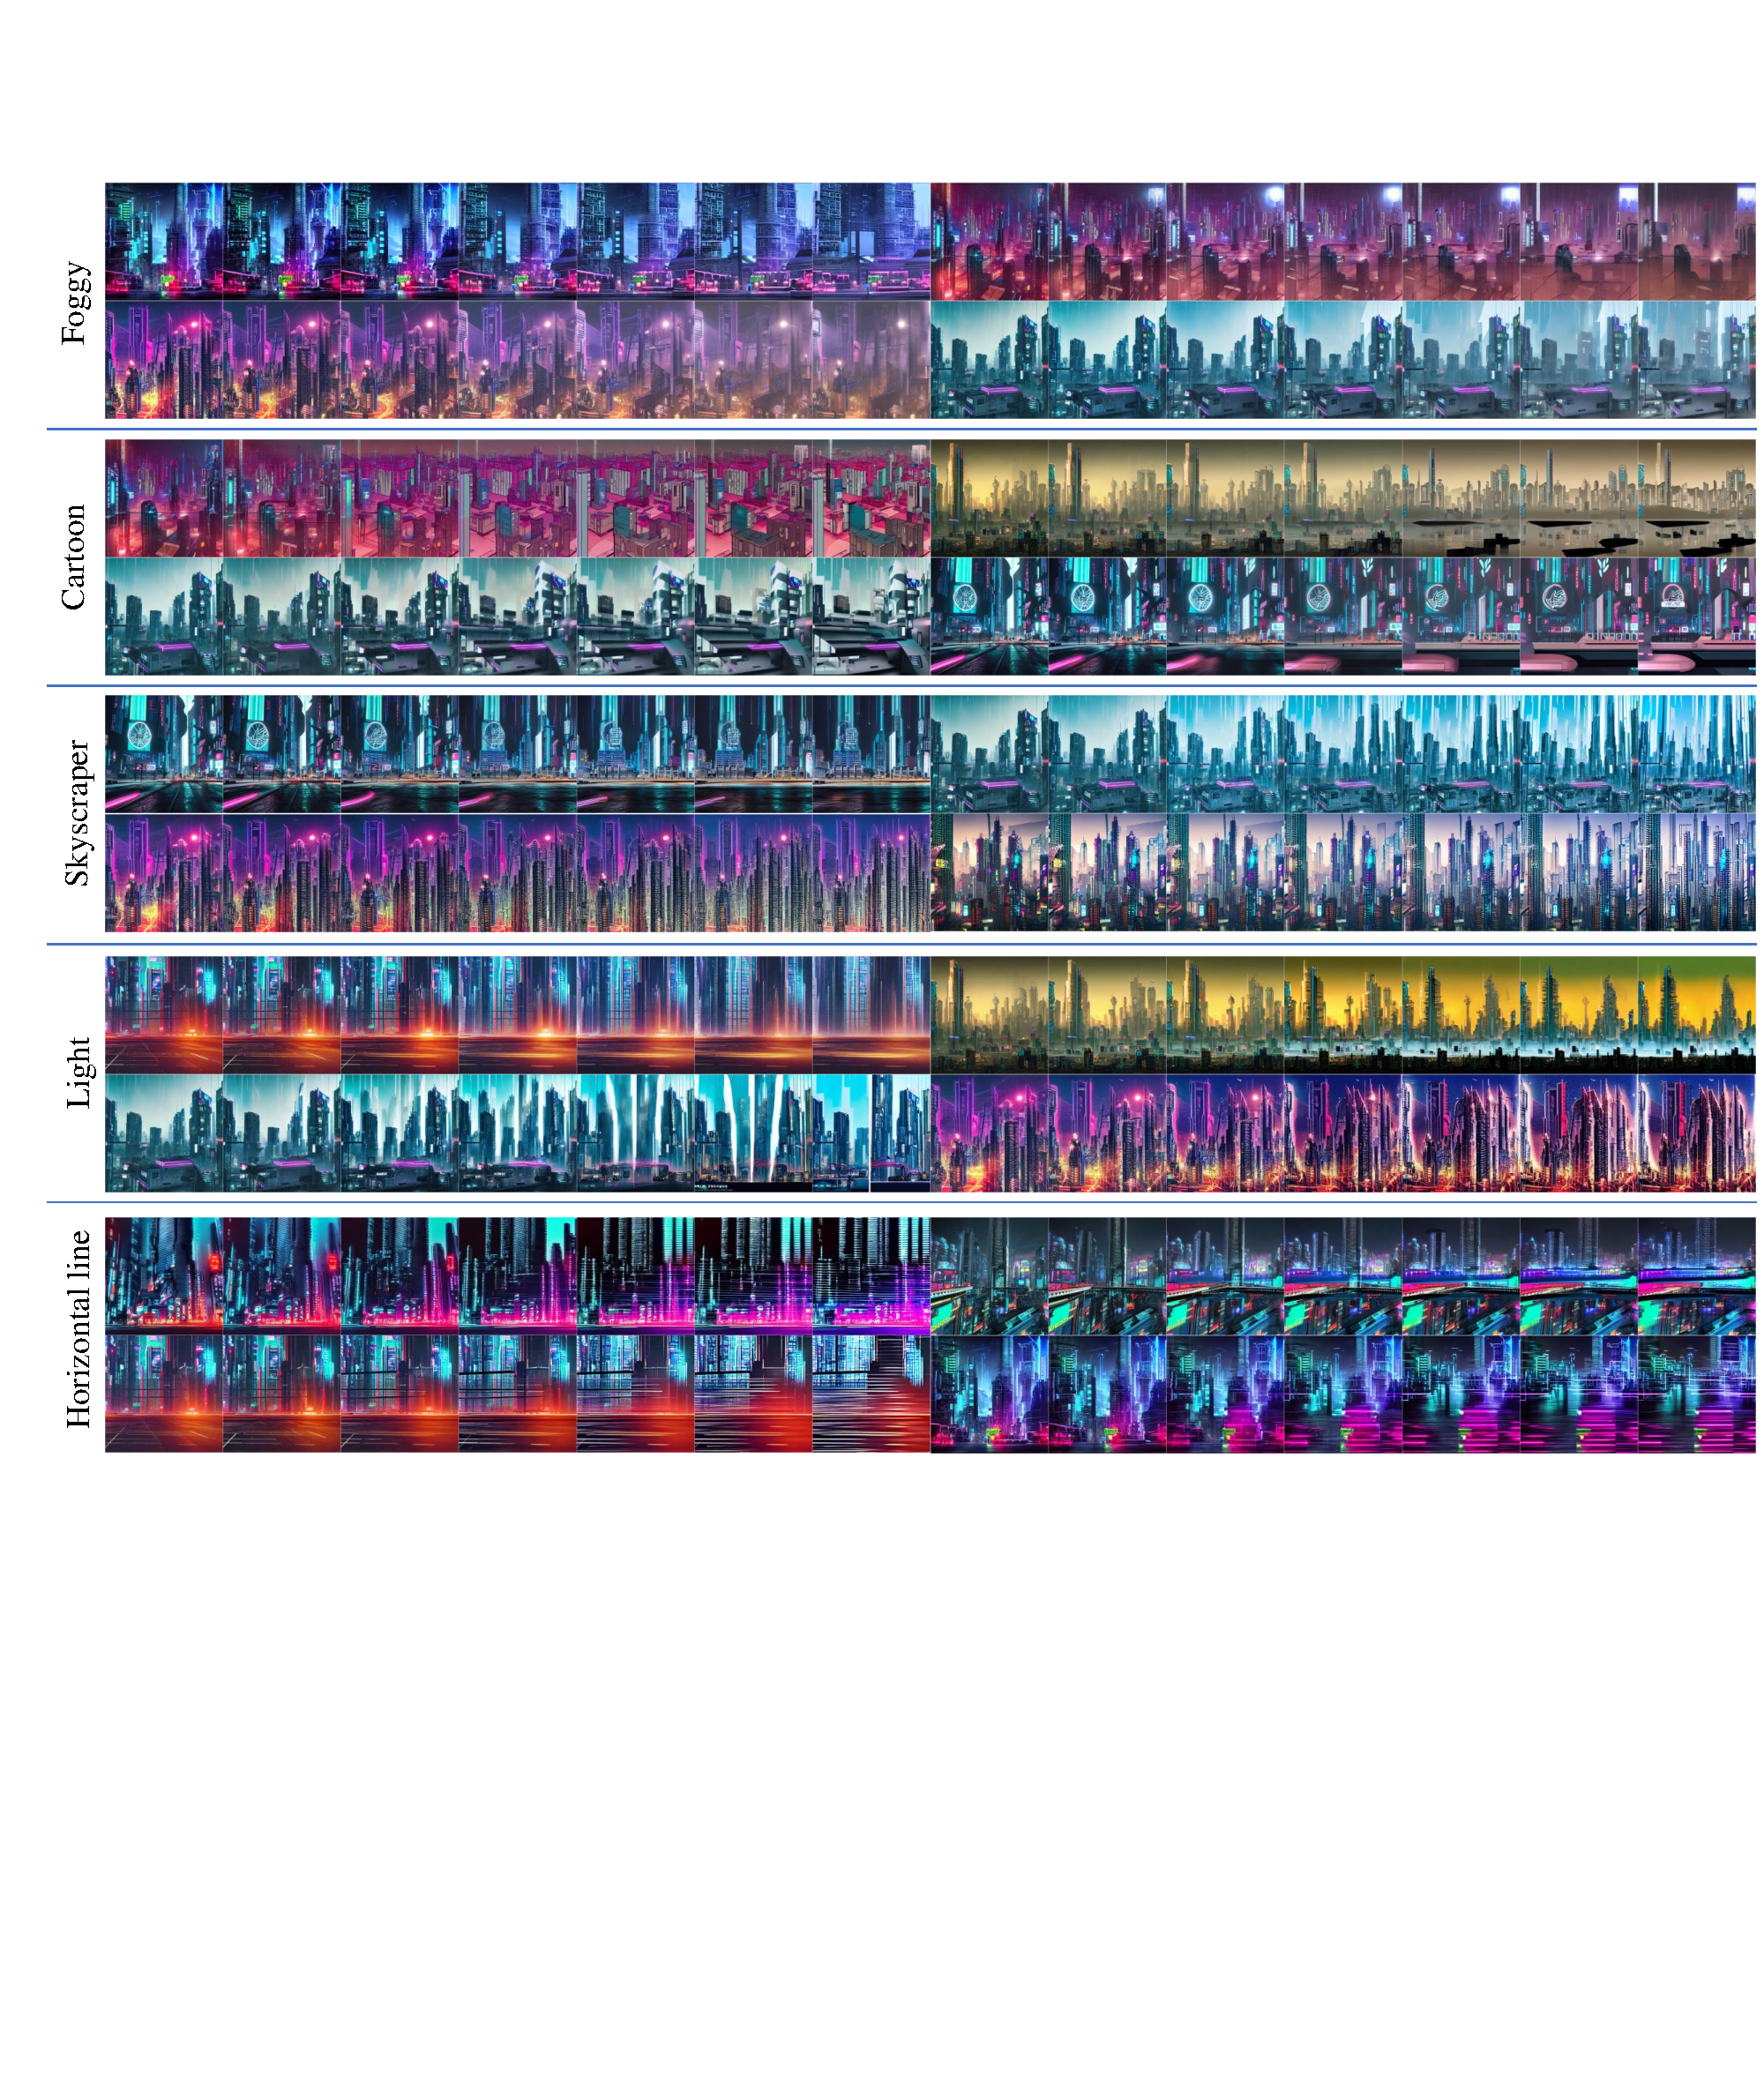
\includegraphics[width=1.0\linewidth]{figure/LDM_global_appendix.pdf}
%     \caption{
%     A selection of interpretable edits discovered by our global feature direction in LDM with "Cyberpunk city". The image on the far left represents the reconstructed original image, while the subsequent images demonstrate the interpretable edits that have been made to it.}
%     \label{fig:LDM_global_appendix}
% \end{figure}


